\label{sec:appendix_A}

The following figures shows the distribution of the kinematic input parameter of the \gls{BDT} training. For each parameter always two plots are shown, first the a signal free plot with events \gls{m_vis} $< 60$ GeV and the inclusive plot with signal drawn. 

\section*{Plot for the $e\mu$ final state}

\begin{figure}[htp]
	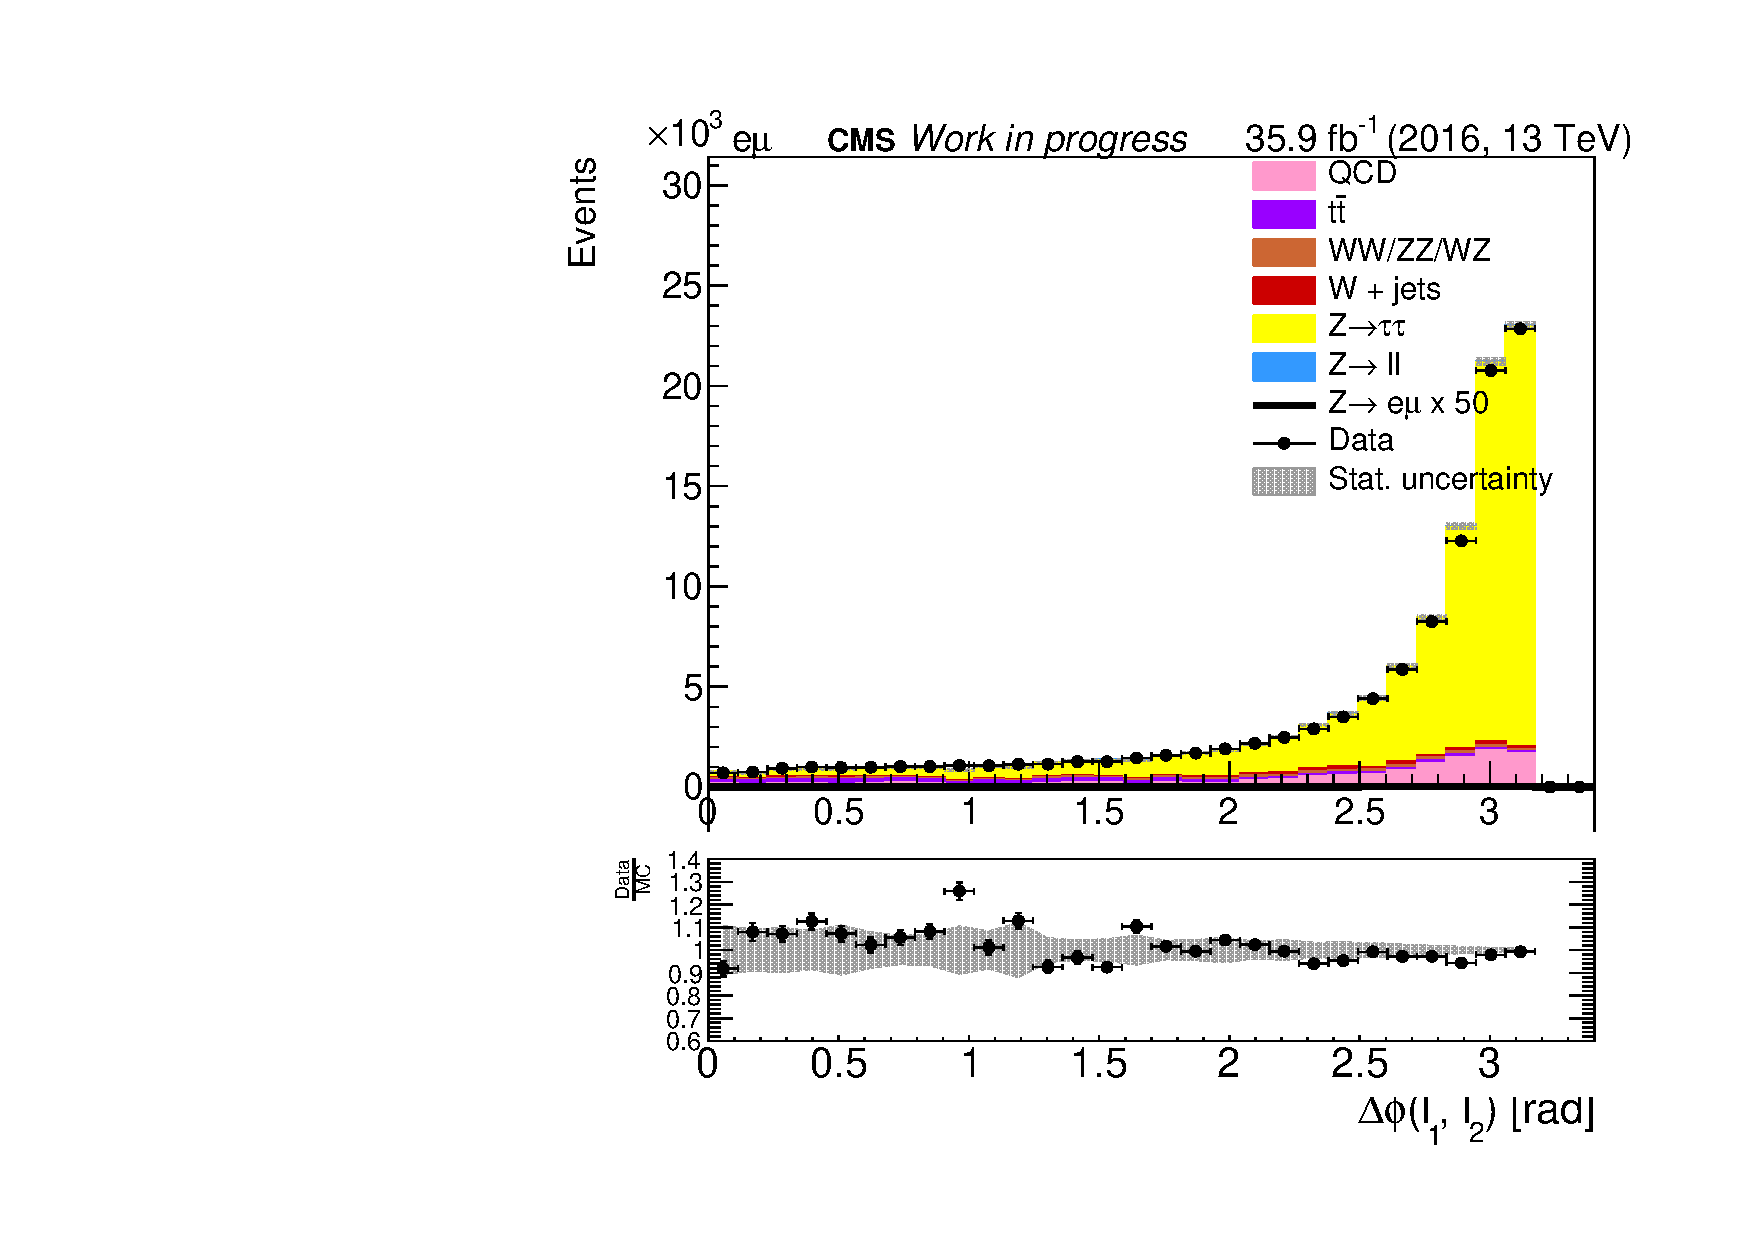
\includegraphics[width=0.45\textwidth]{plots/em/DeltaPhiL1L2_CR.pdf}
	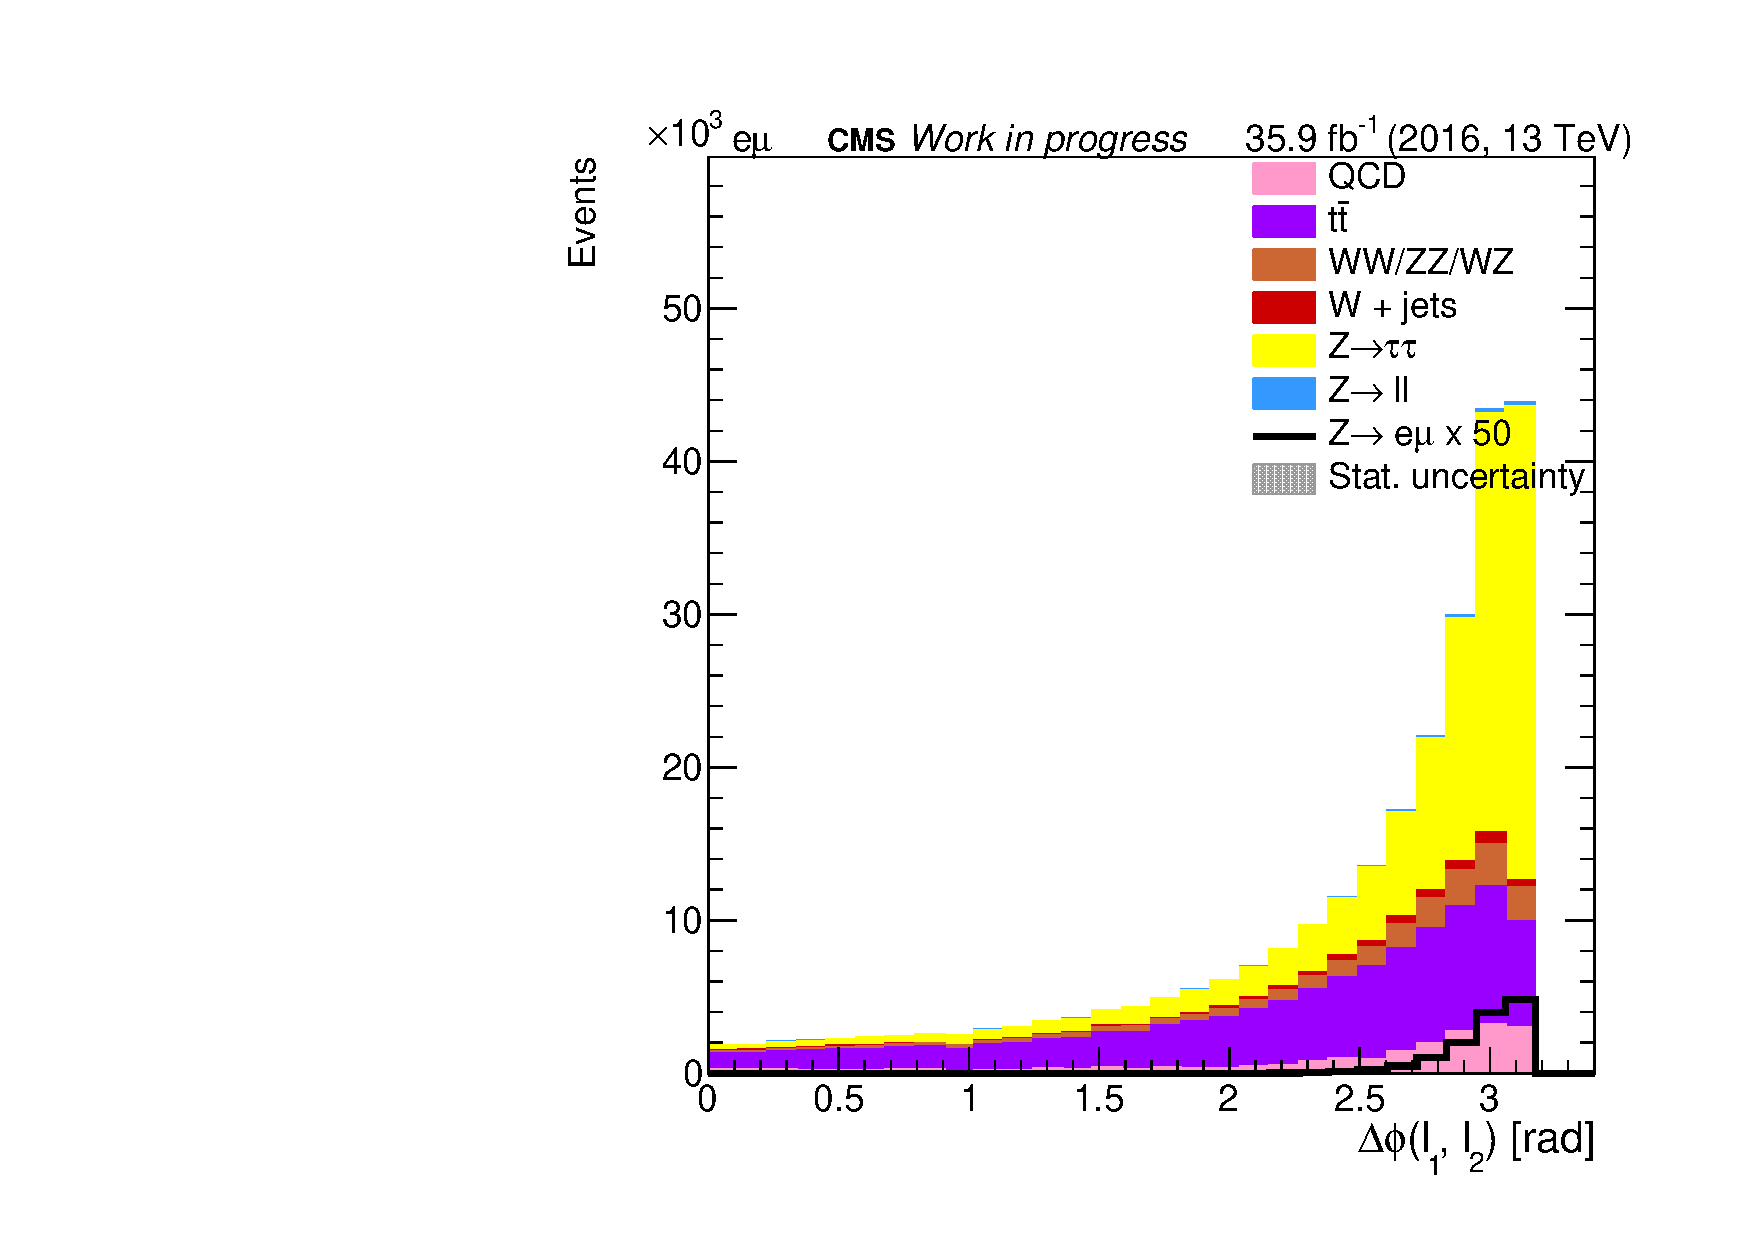
\includegraphics[width=0.45\textwidth]{plots/em/DeltaPhiL1L2_withsignal.pdf}

	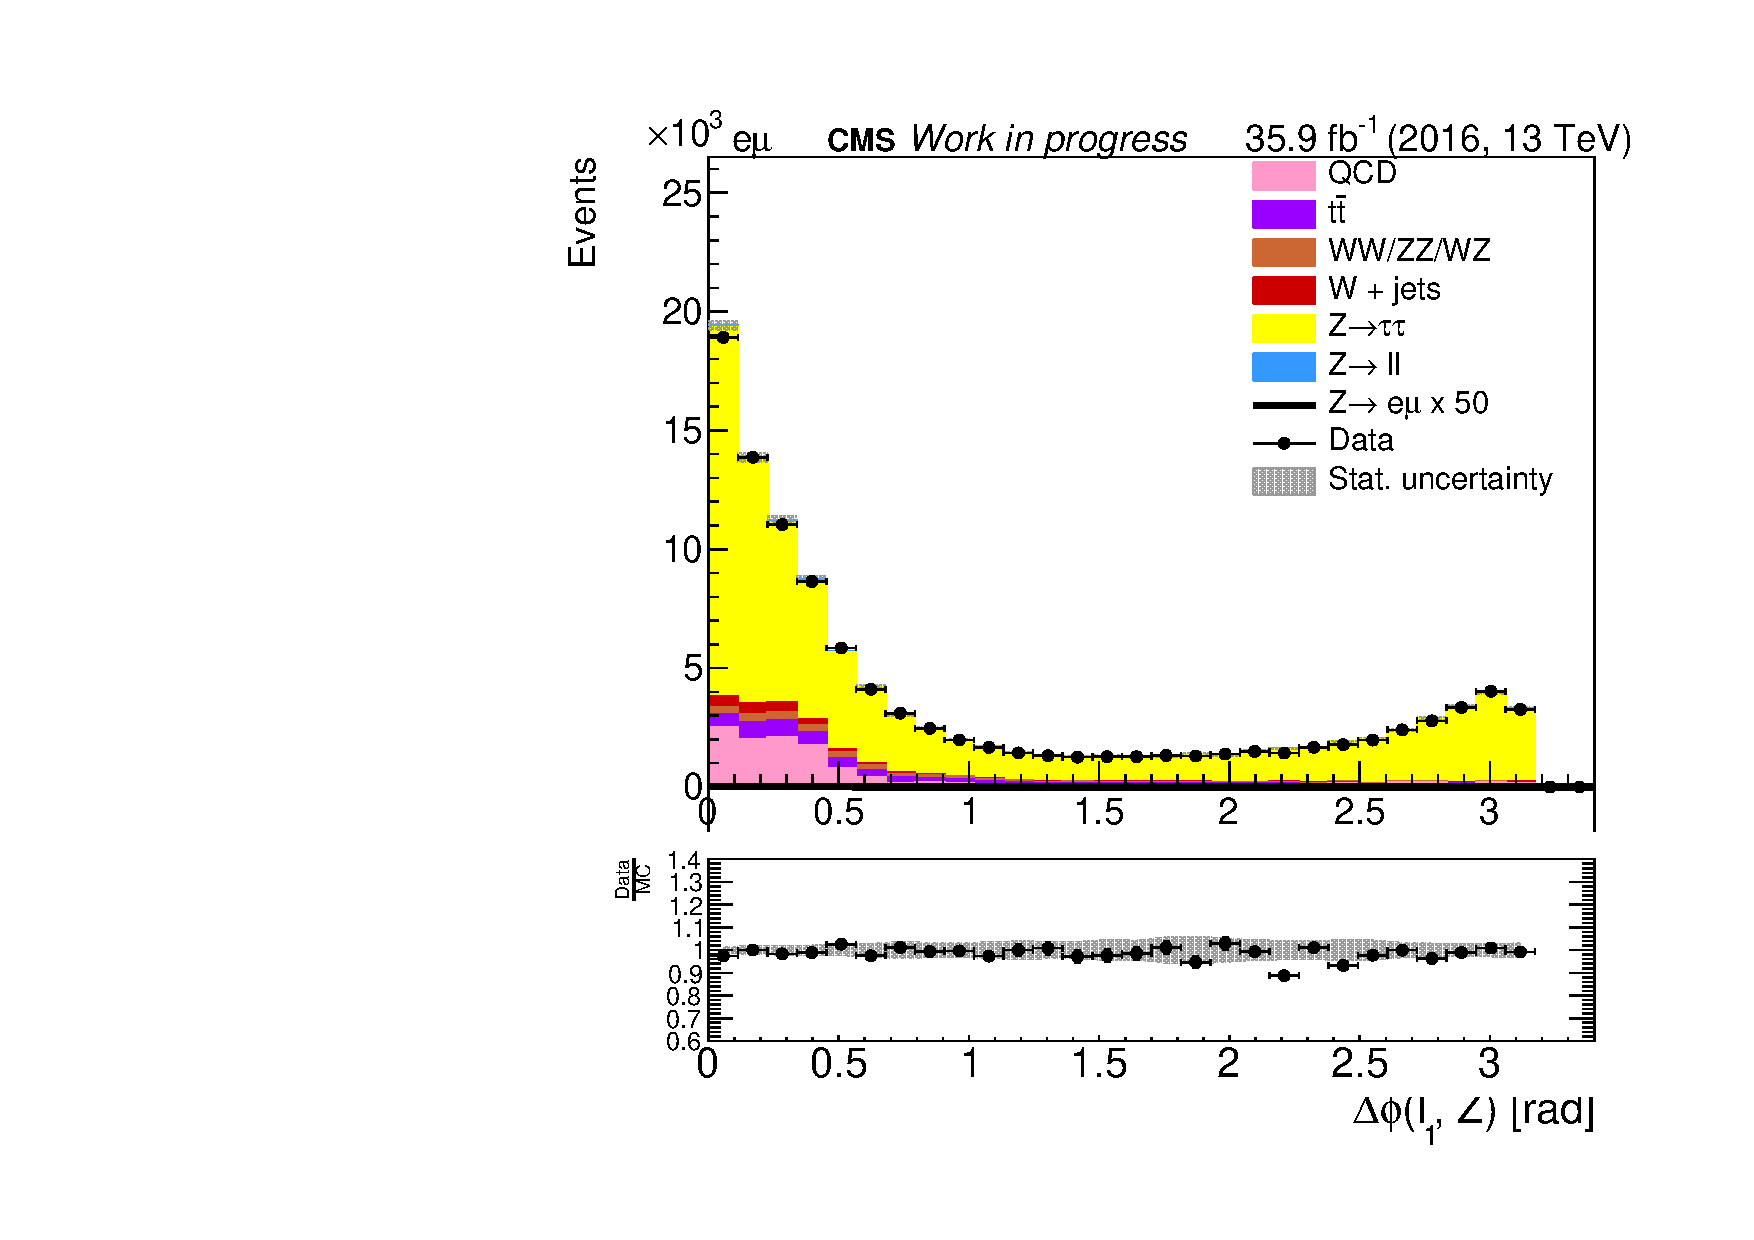
\includegraphics[width=0.45\textwidth]{plots/em/DeltaPhiL1Z_CR.pdf}
	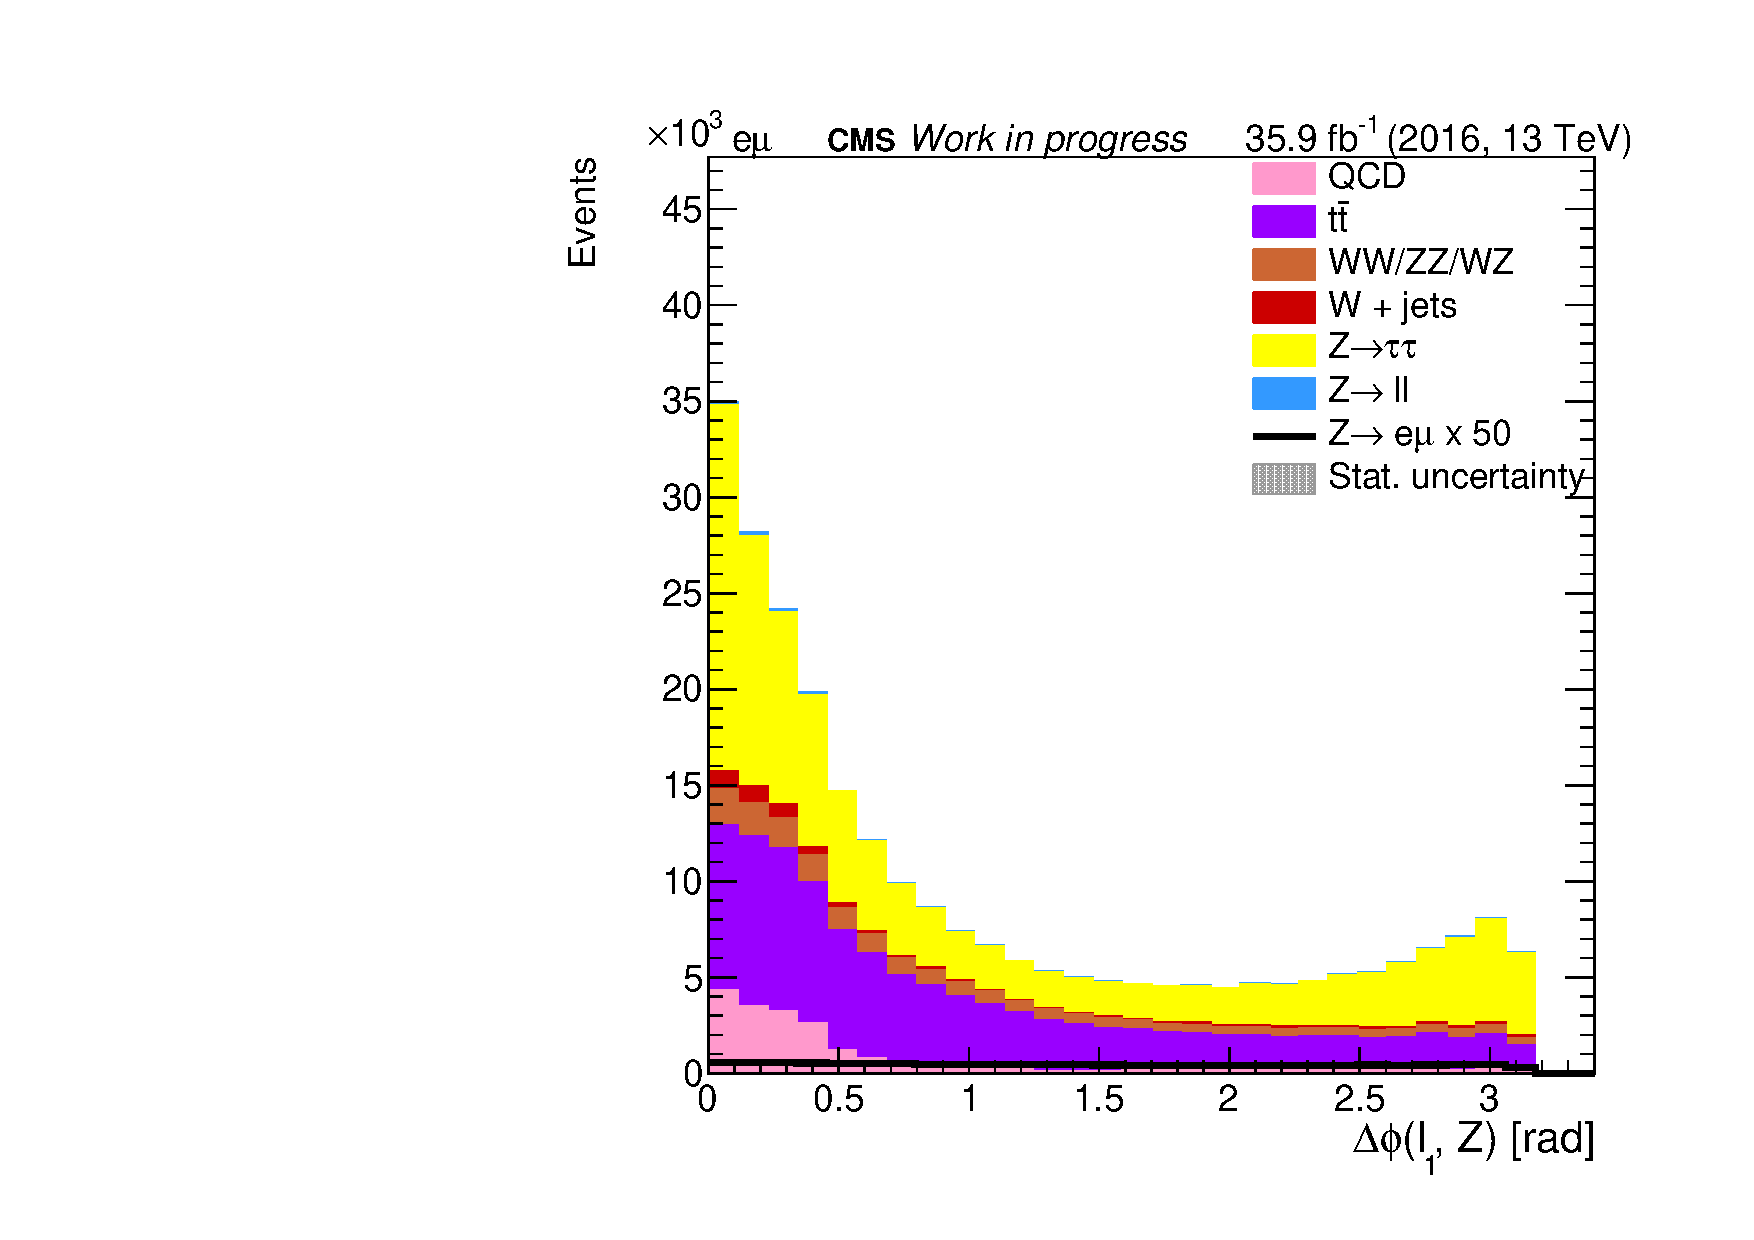
\includegraphics[width=0.45\textwidth]{plots/em/DeltaPhiL1Z_withsignal.pdf}

\end{figure}


\begin{figure}[htp]
	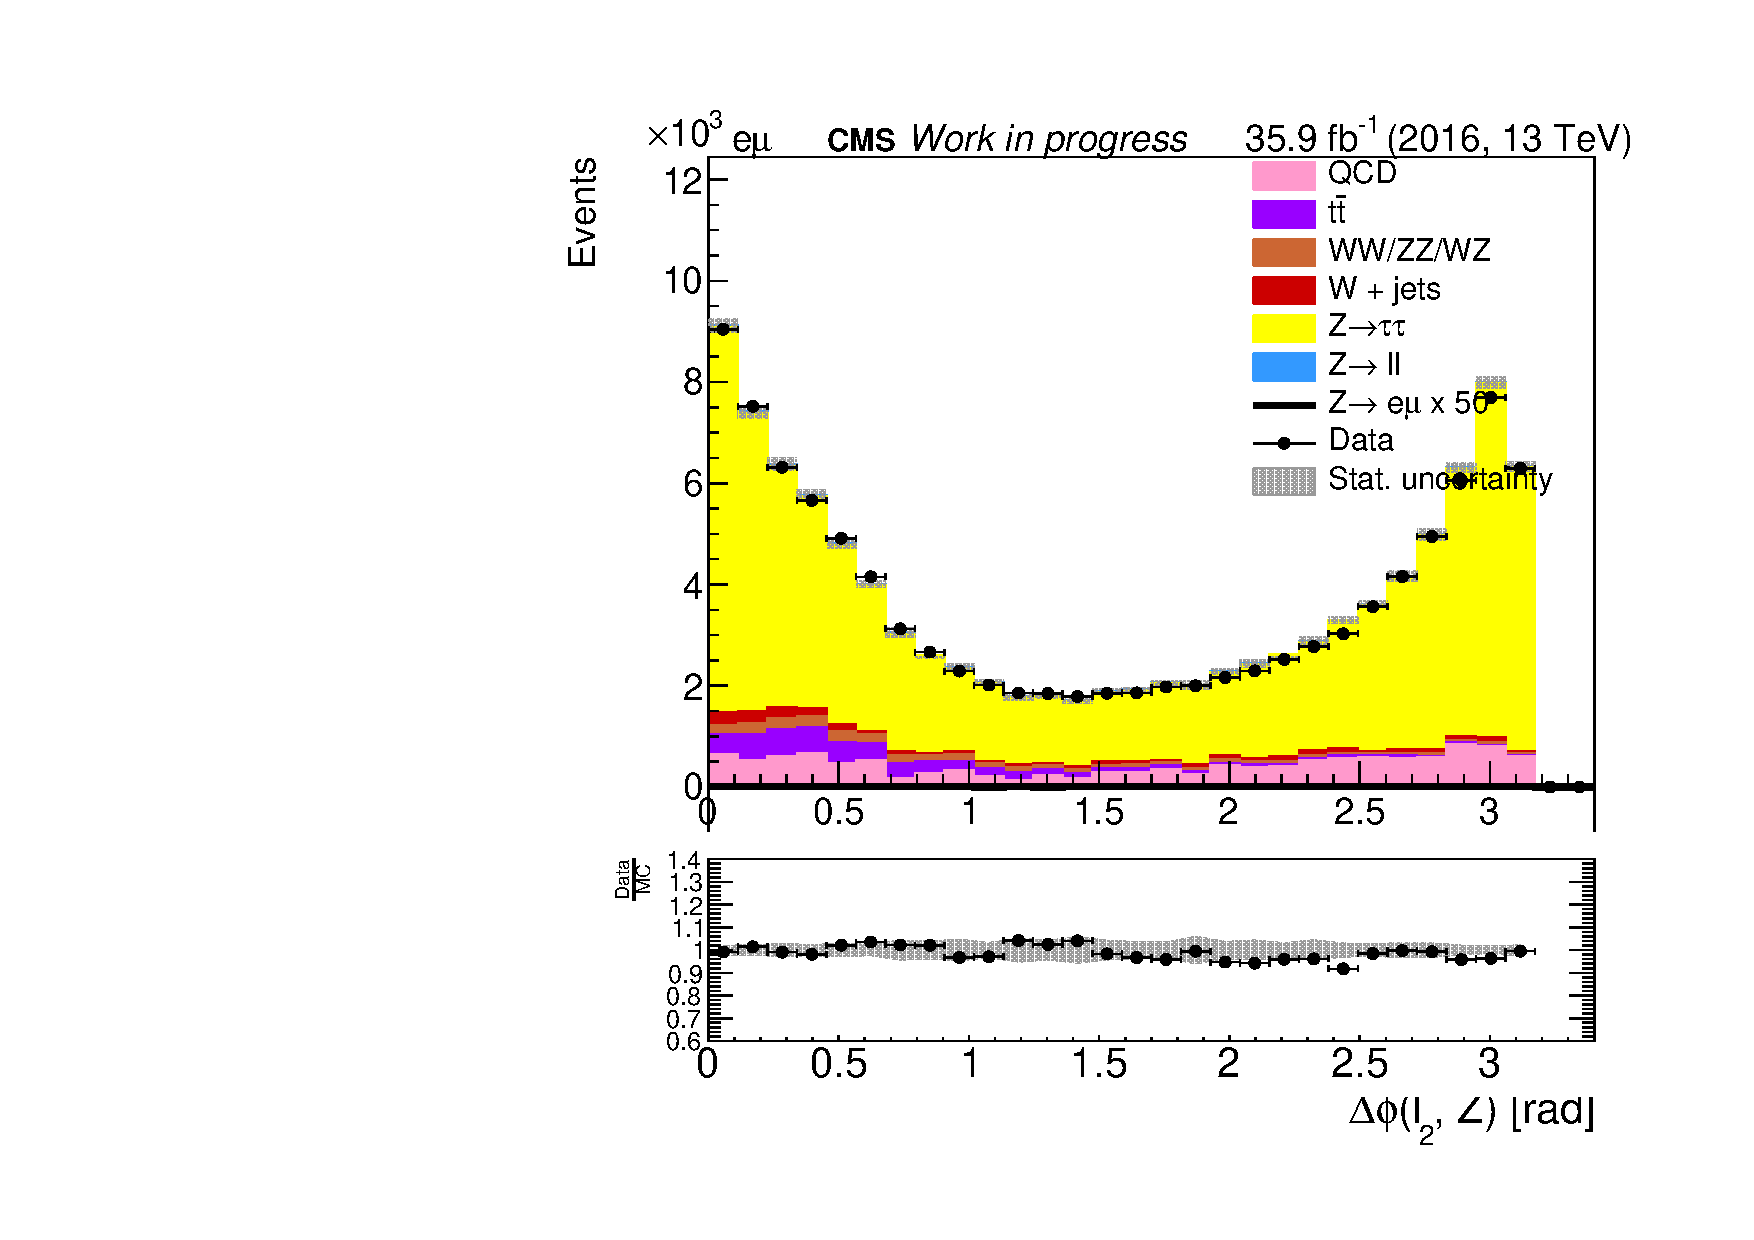
\includegraphics[width=0.45\textwidth]{plots/em/DeltaPhiL2Z_CR.pdf}
	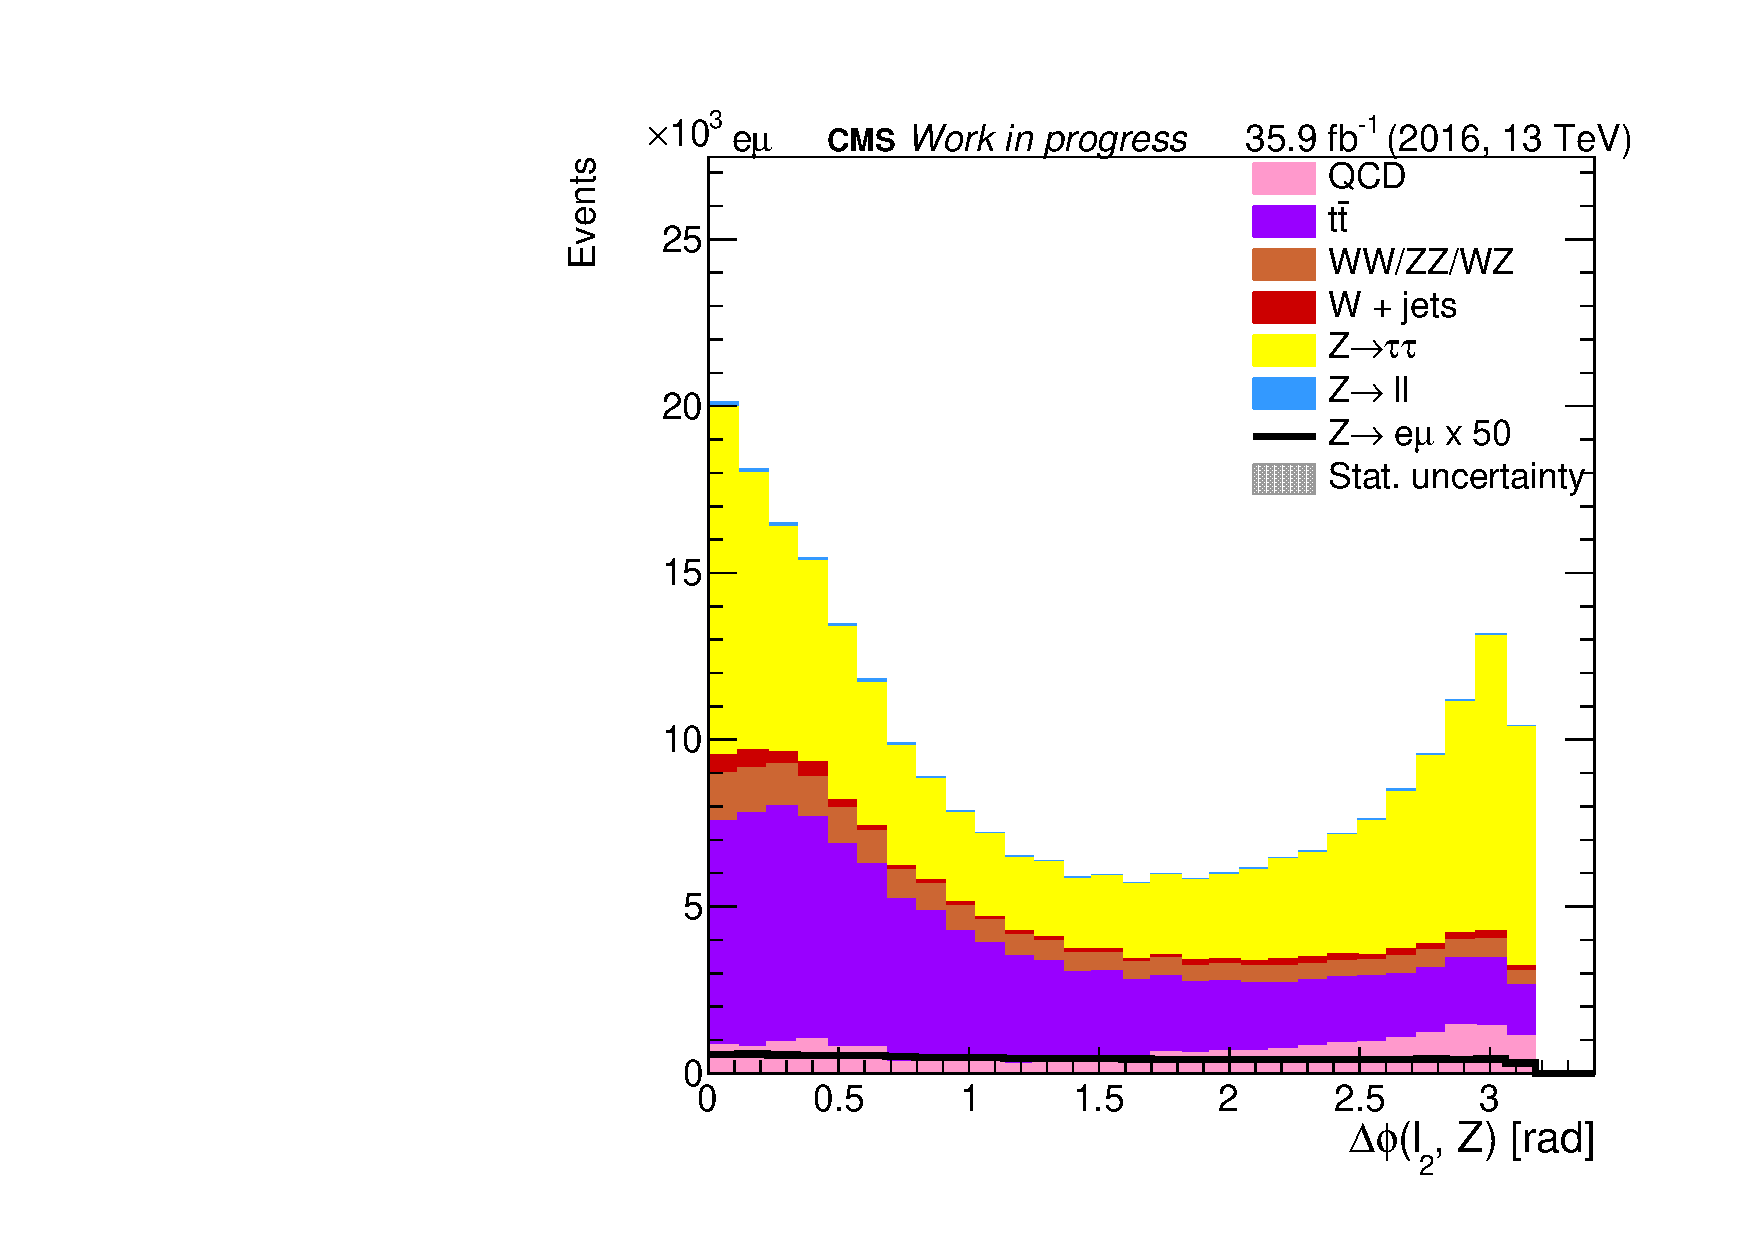
\includegraphics[width=0.45\textwidth]{plots/em/DeltaPhiL2Z_withsignal.pdf}

	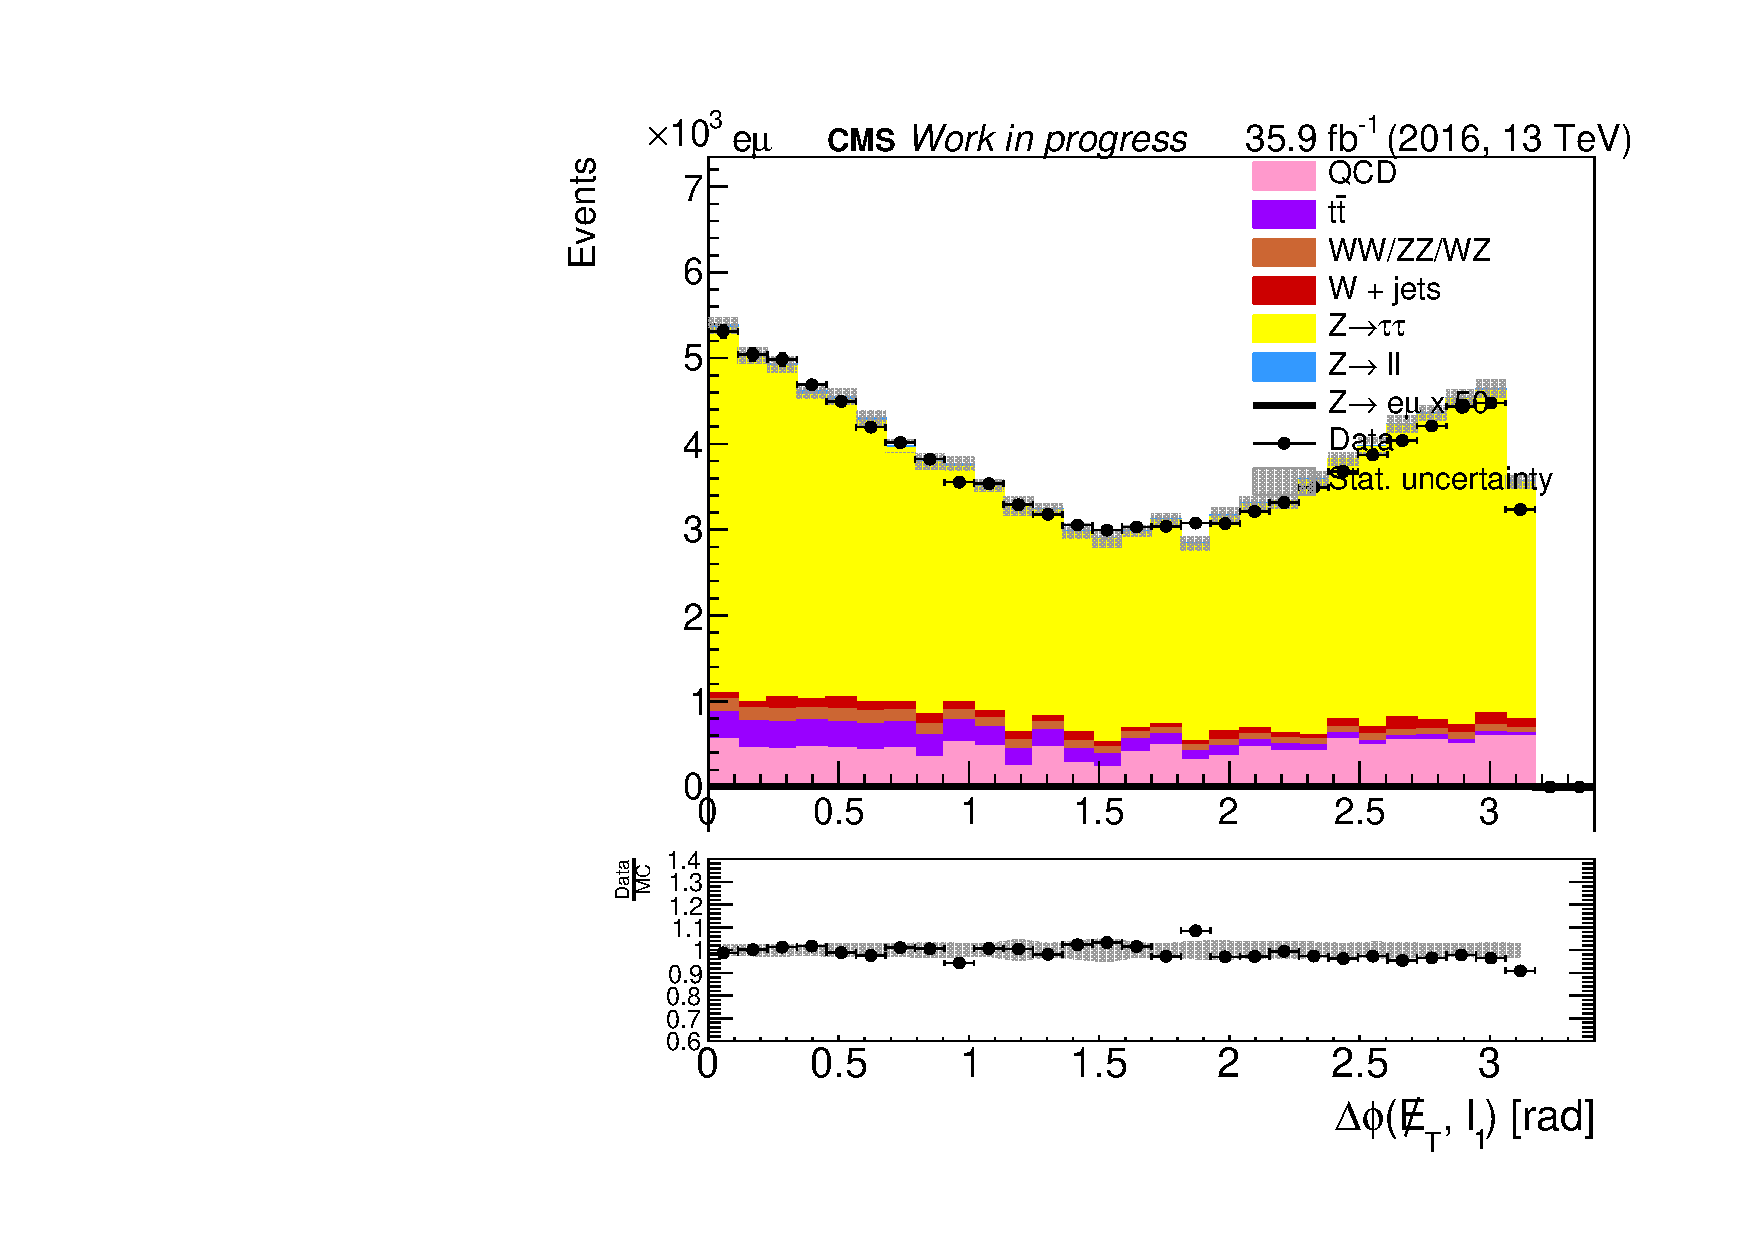
\includegraphics[width=0.45\textwidth]{plots/em/DeltaPhiMetL1_CR.pdf}
	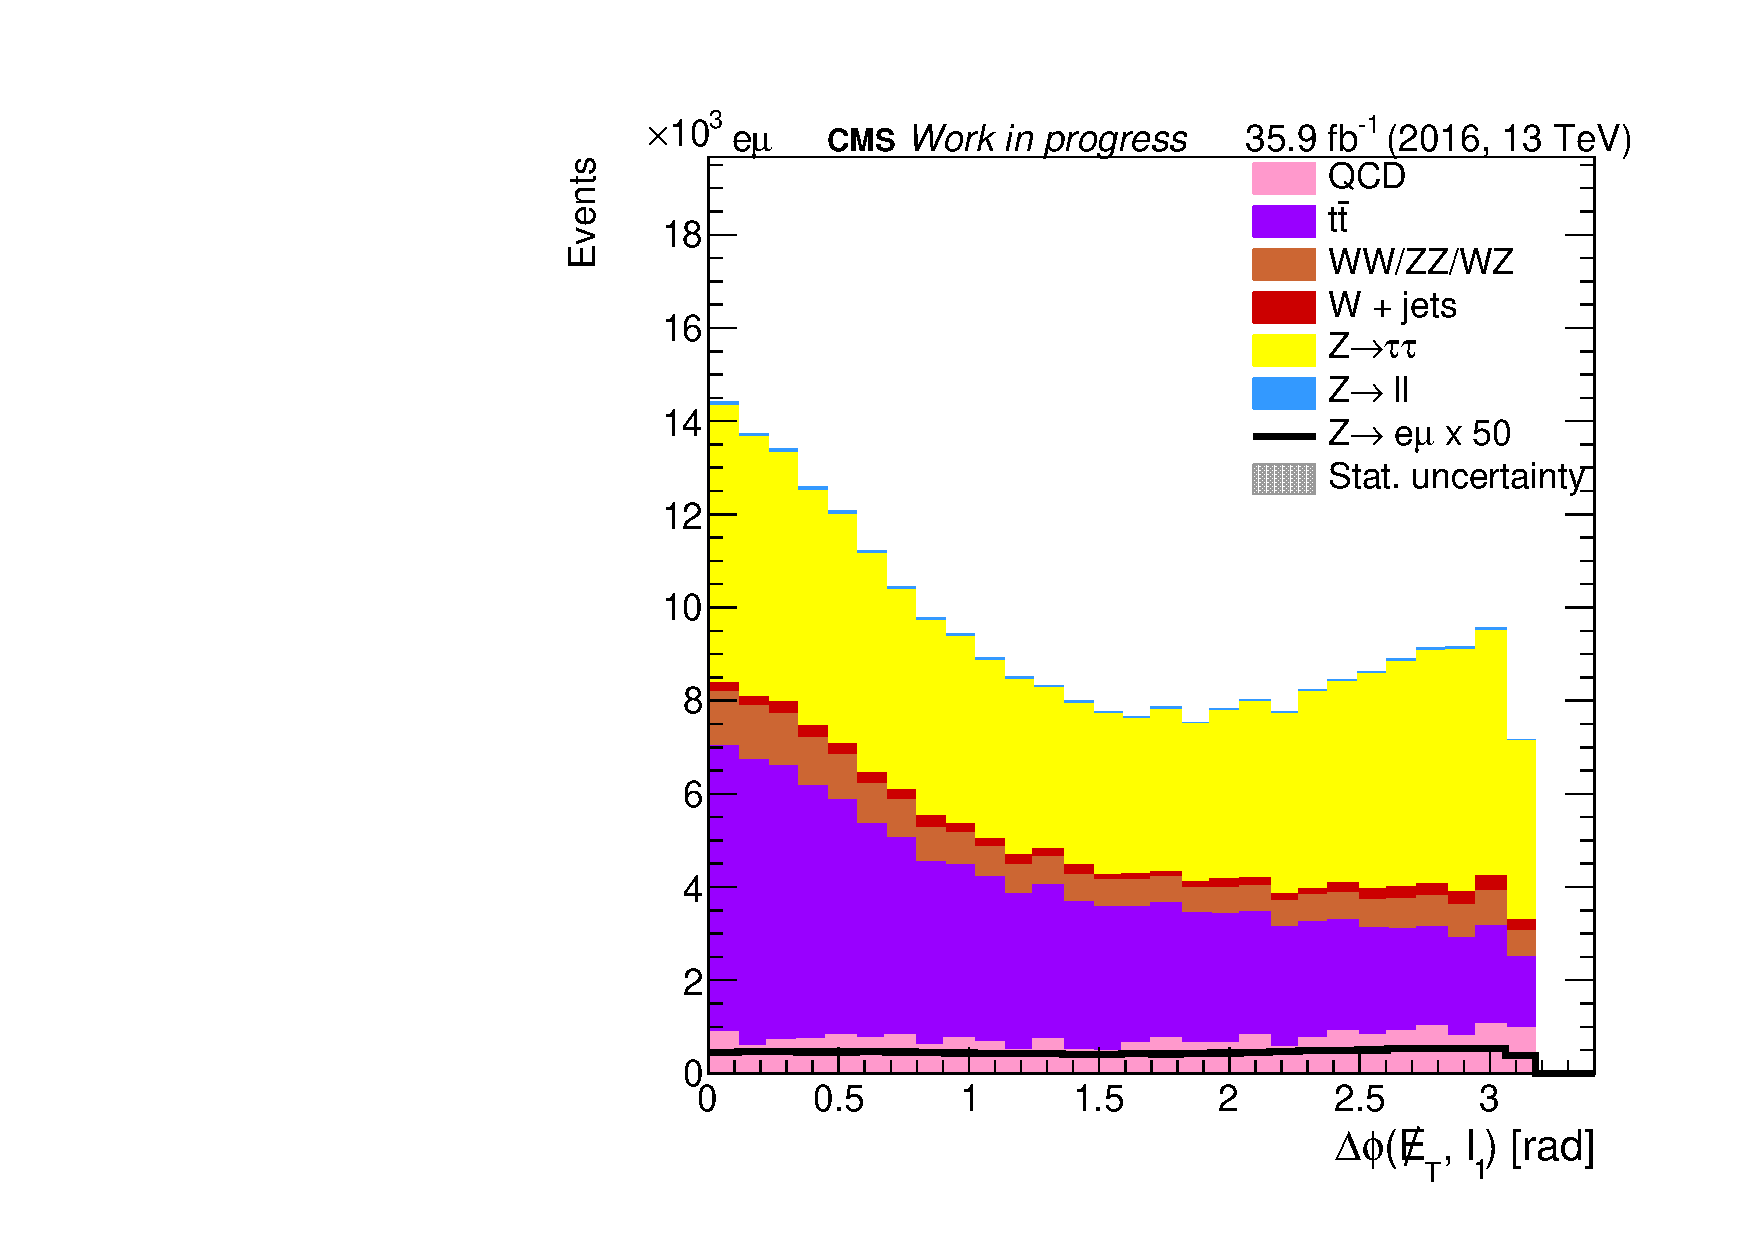
\includegraphics[width=0.45\textwidth]{plots/em/DeltaPhiMetL1_withsignal.pdf}

	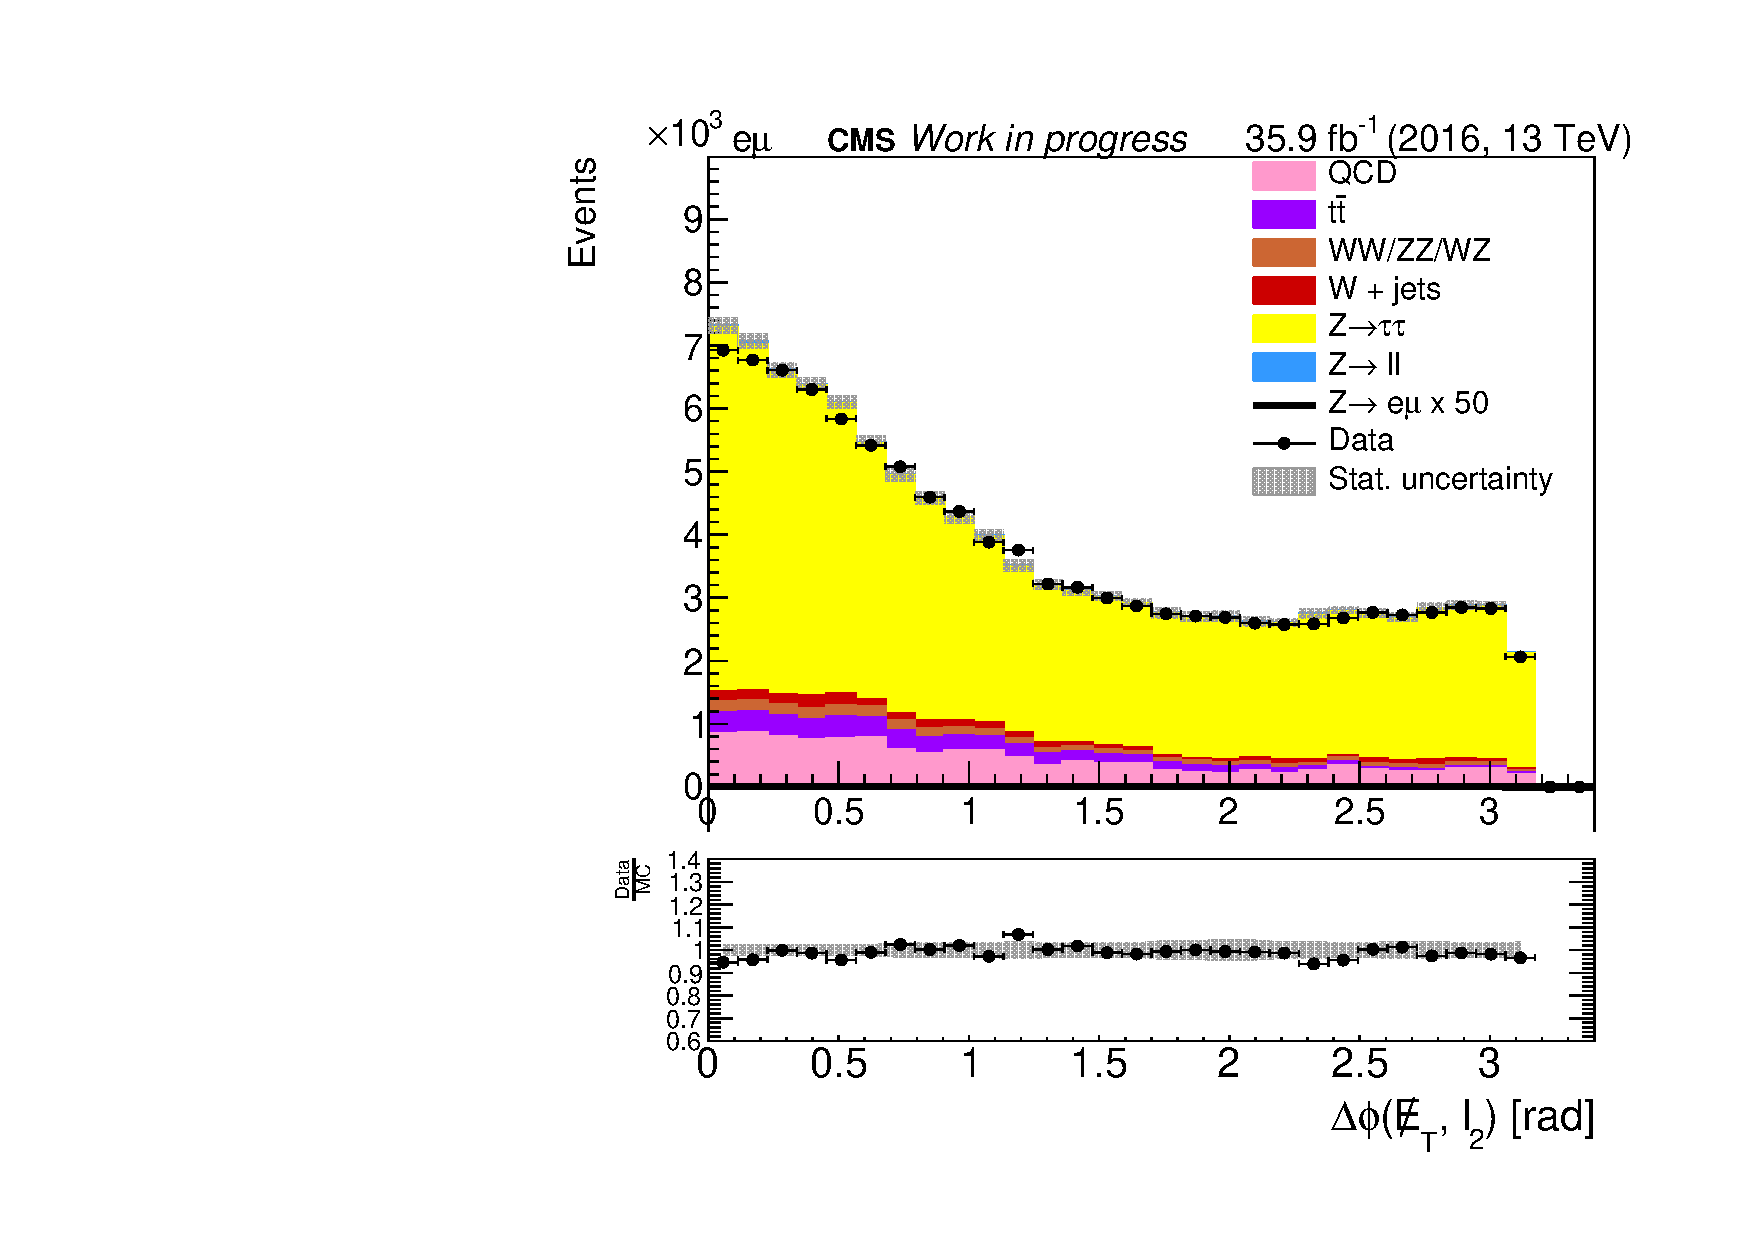
\includegraphics[width=0.45\textwidth]{plots/em/DeltaPhiMetL2_CR.pdf}
	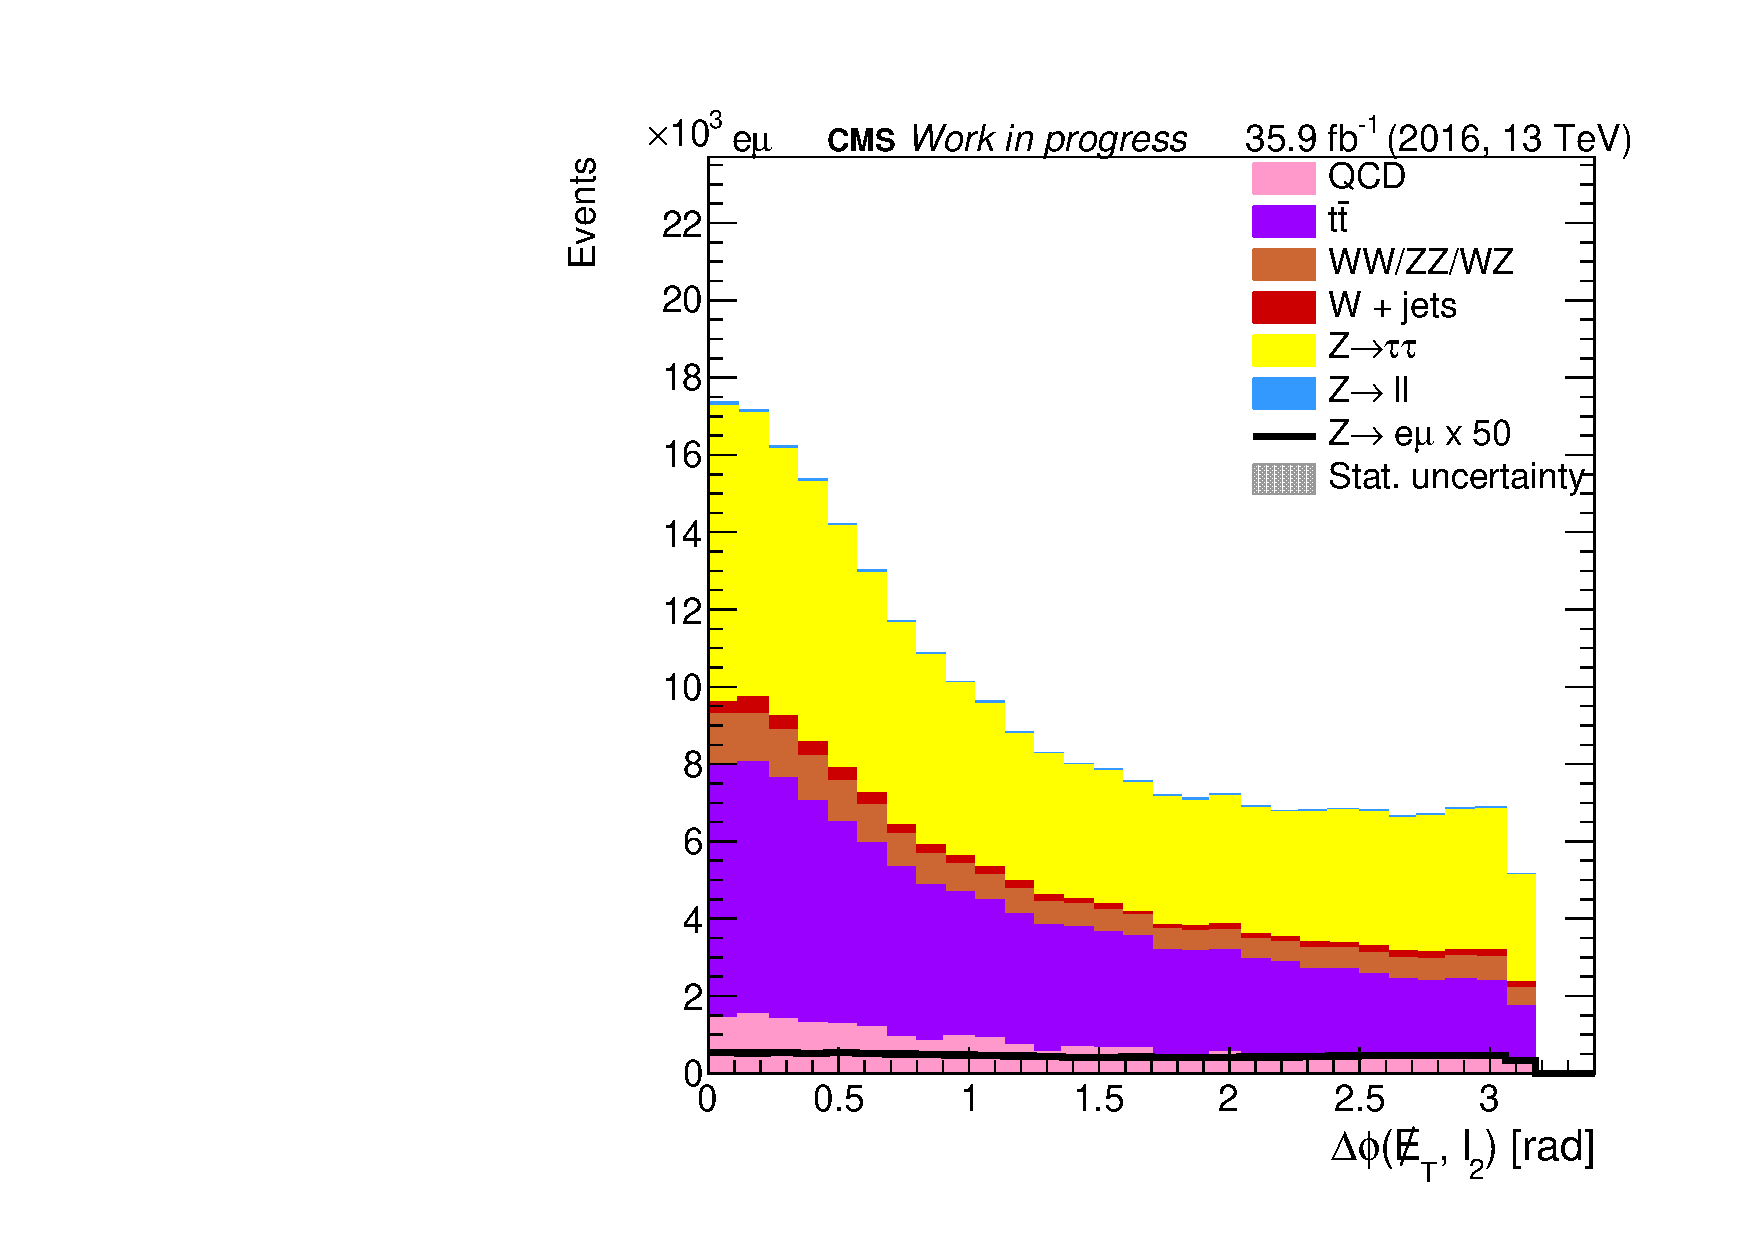
\includegraphics[width=0.45\textwidth]{plots/em/DeltaPhiMetL2_withsignal.pdf}
\end{figure}


\begin{figure}[htp]
	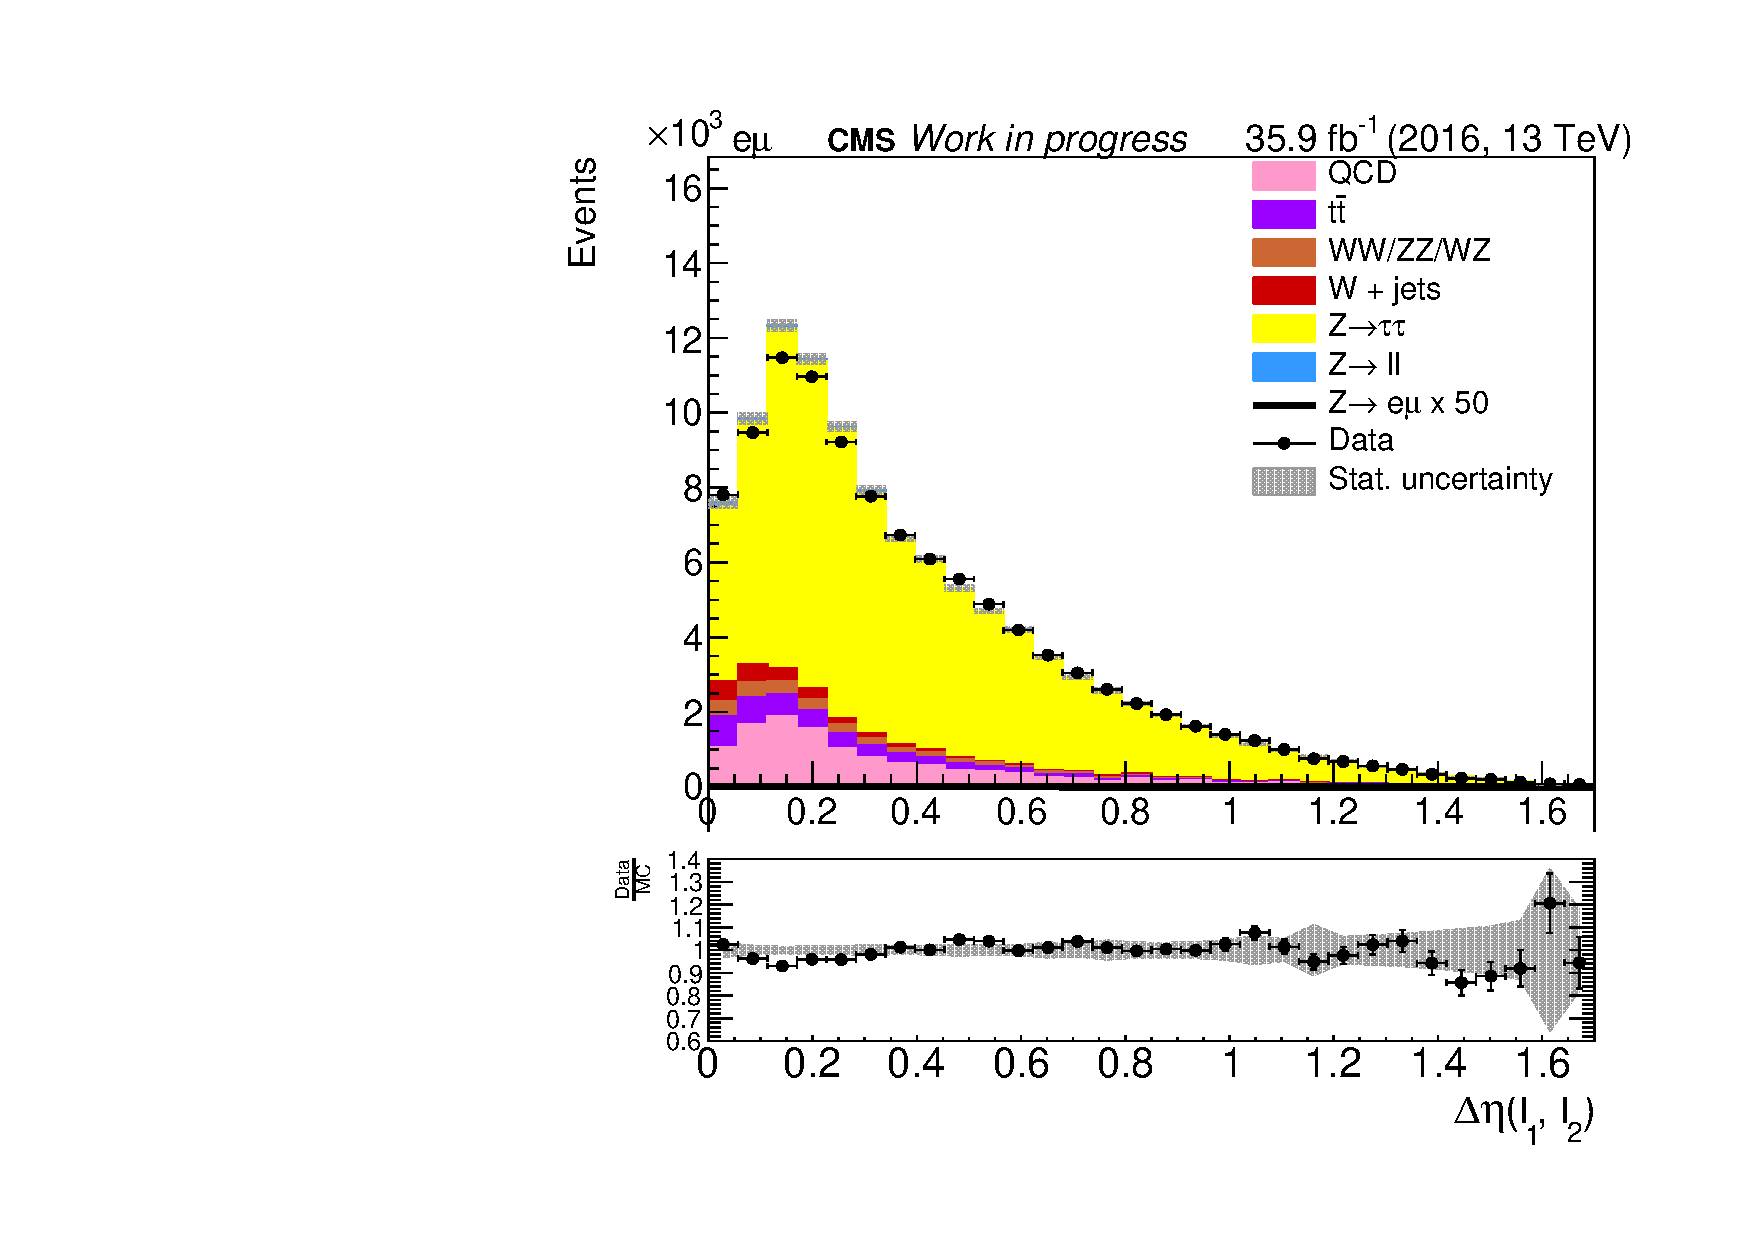
\includegraphics[width=0.45\textwidth]{plots/em/DiEta_CR.pdf}
	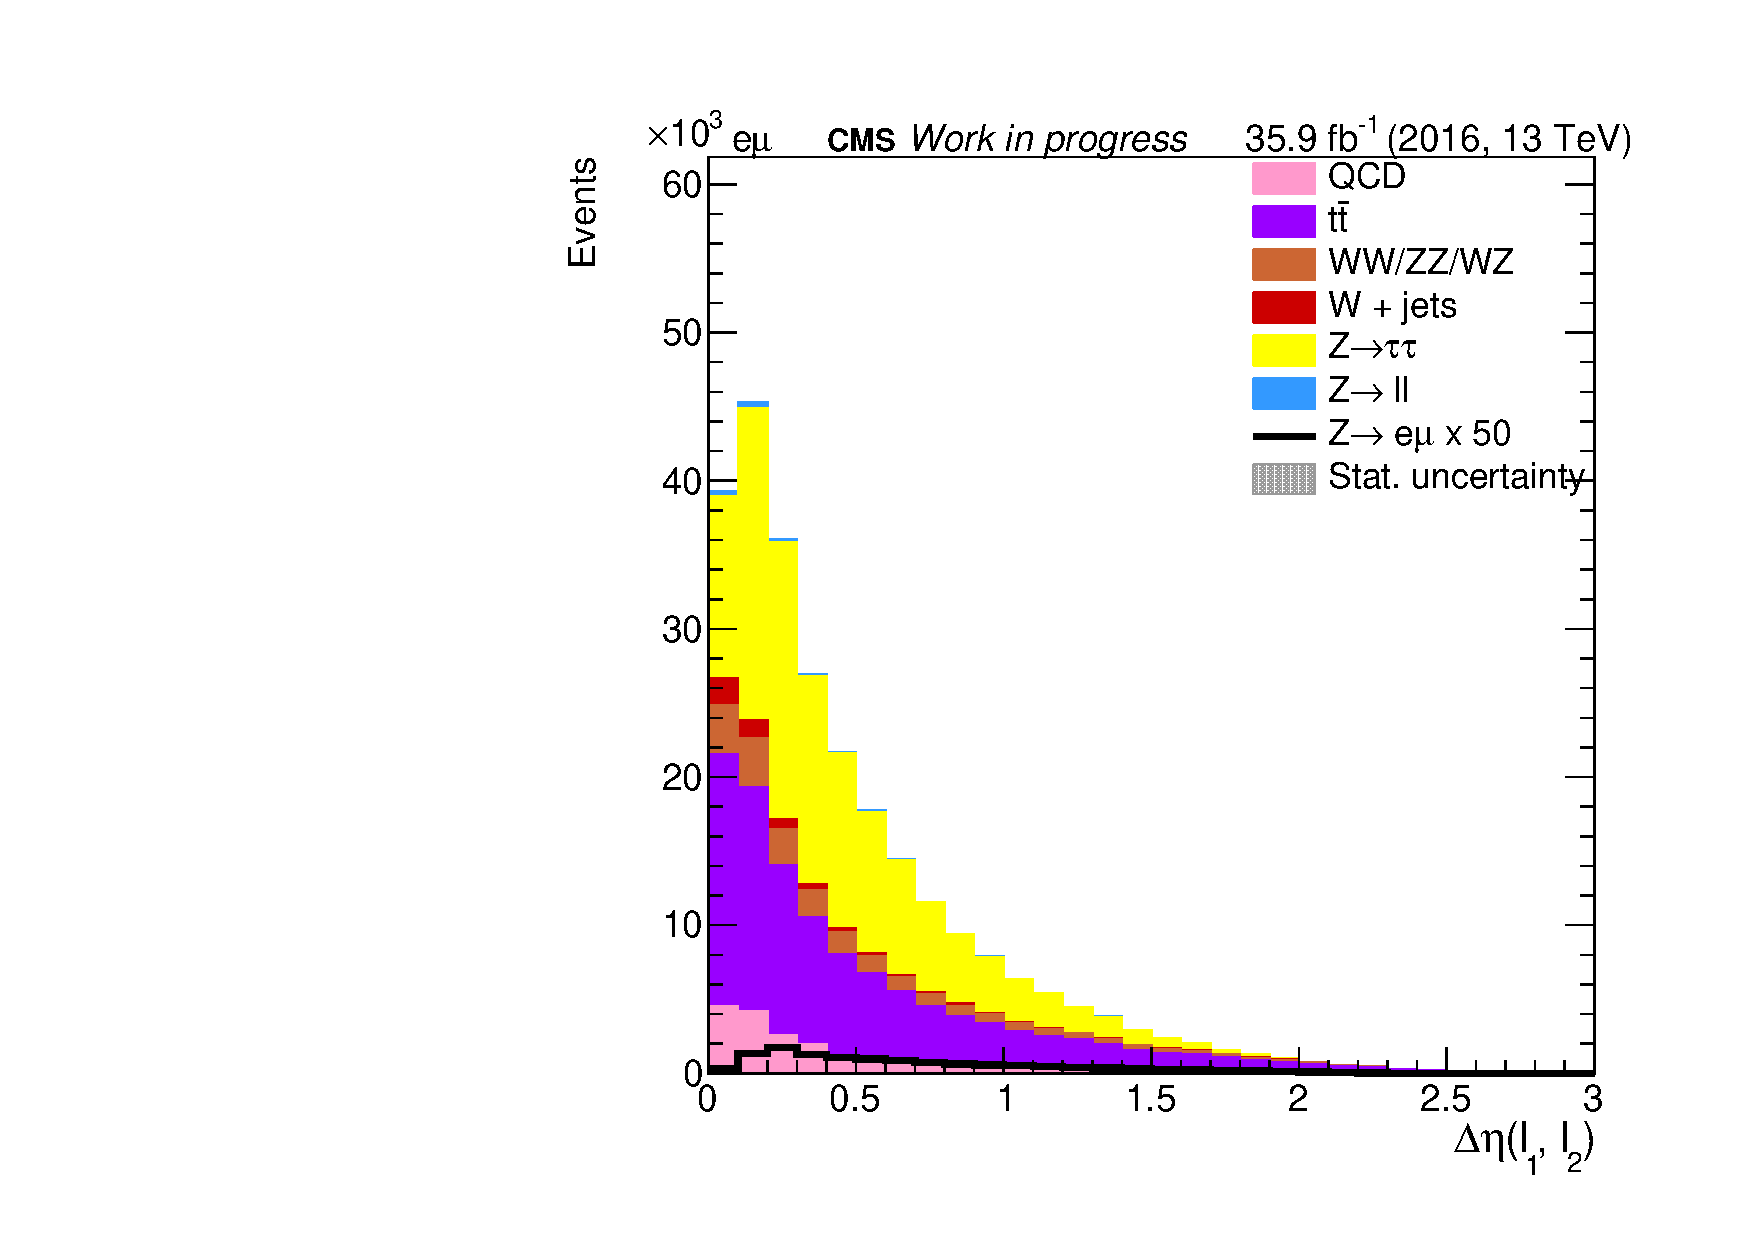
\includegraphics[width=0.45\textwidth]{plots/em/DiEta_withsignal.pdf}

	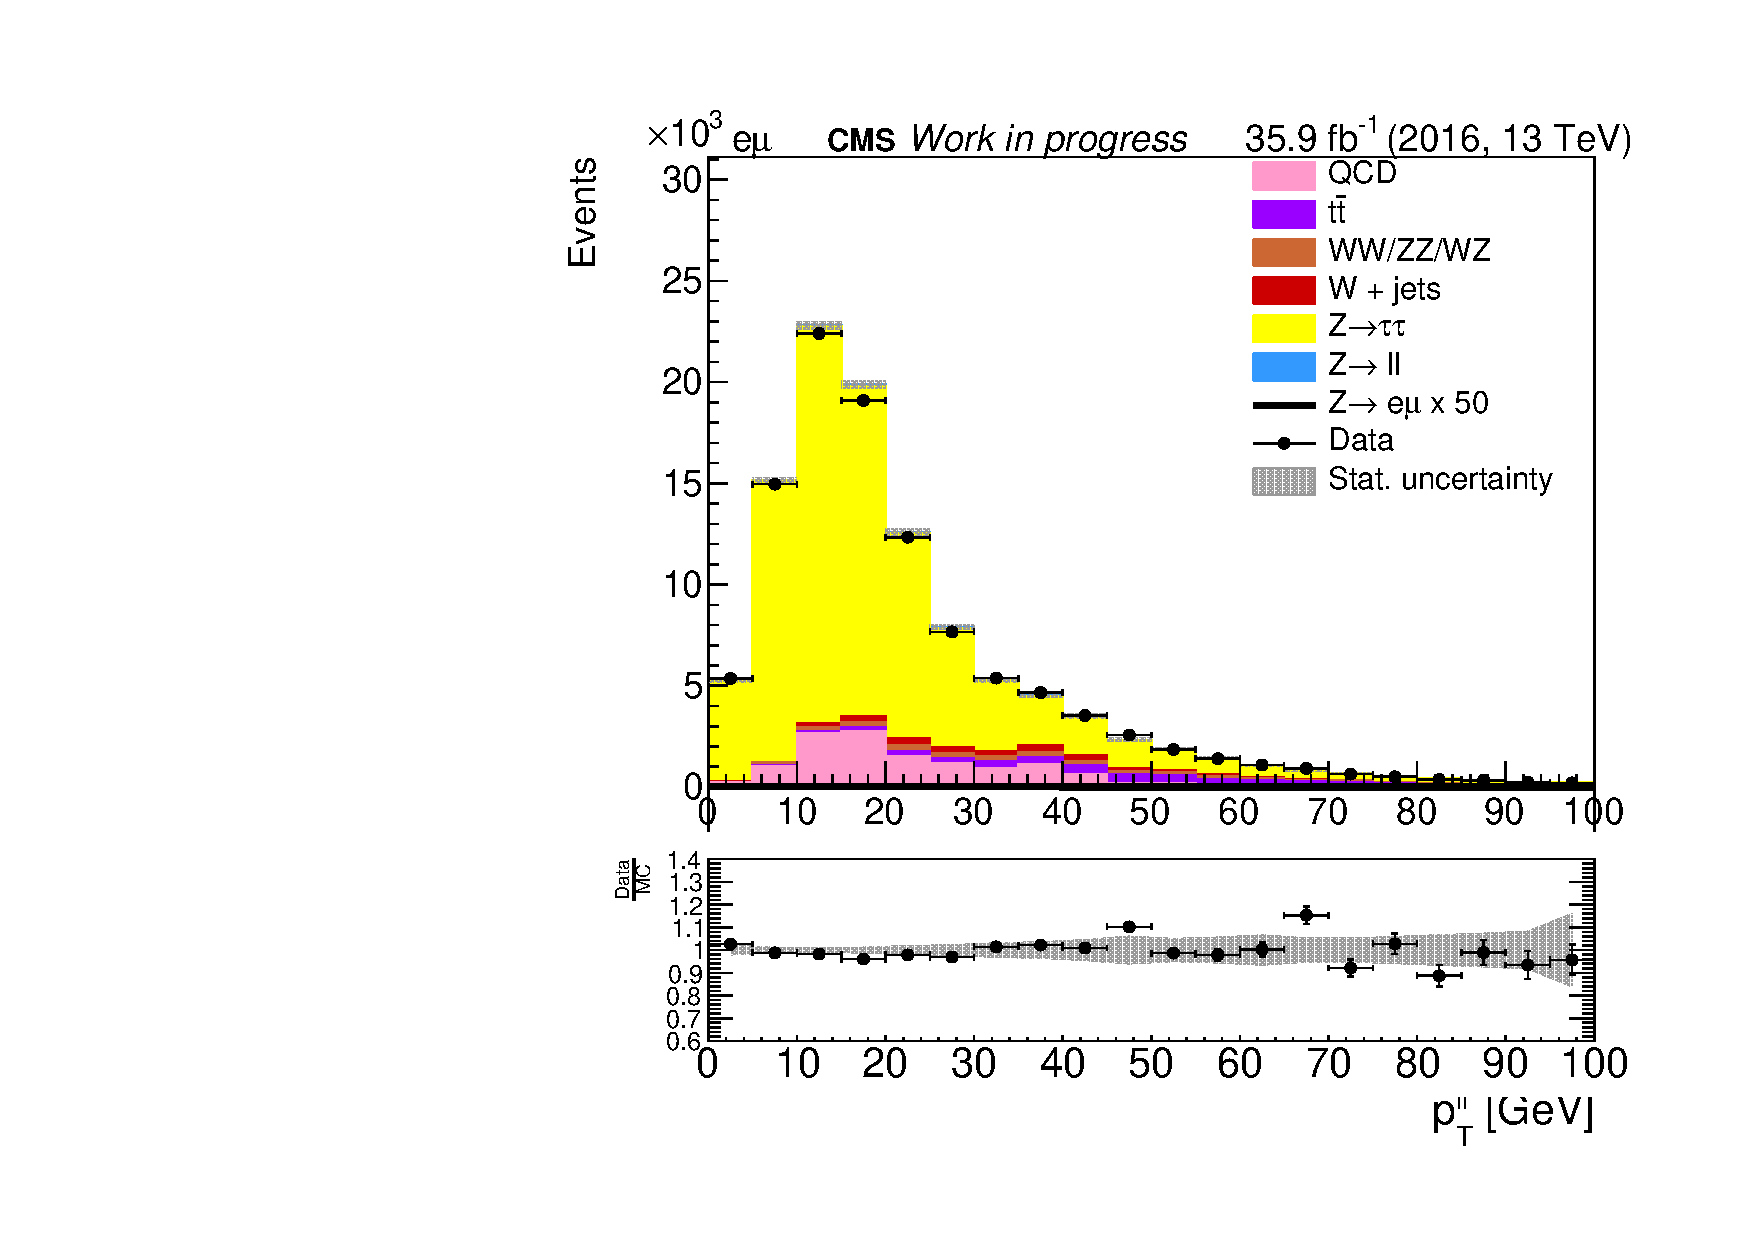
\includegraphics[width=0.45\textwidth]{plots/em/DiLepPt_CR.pdf}
	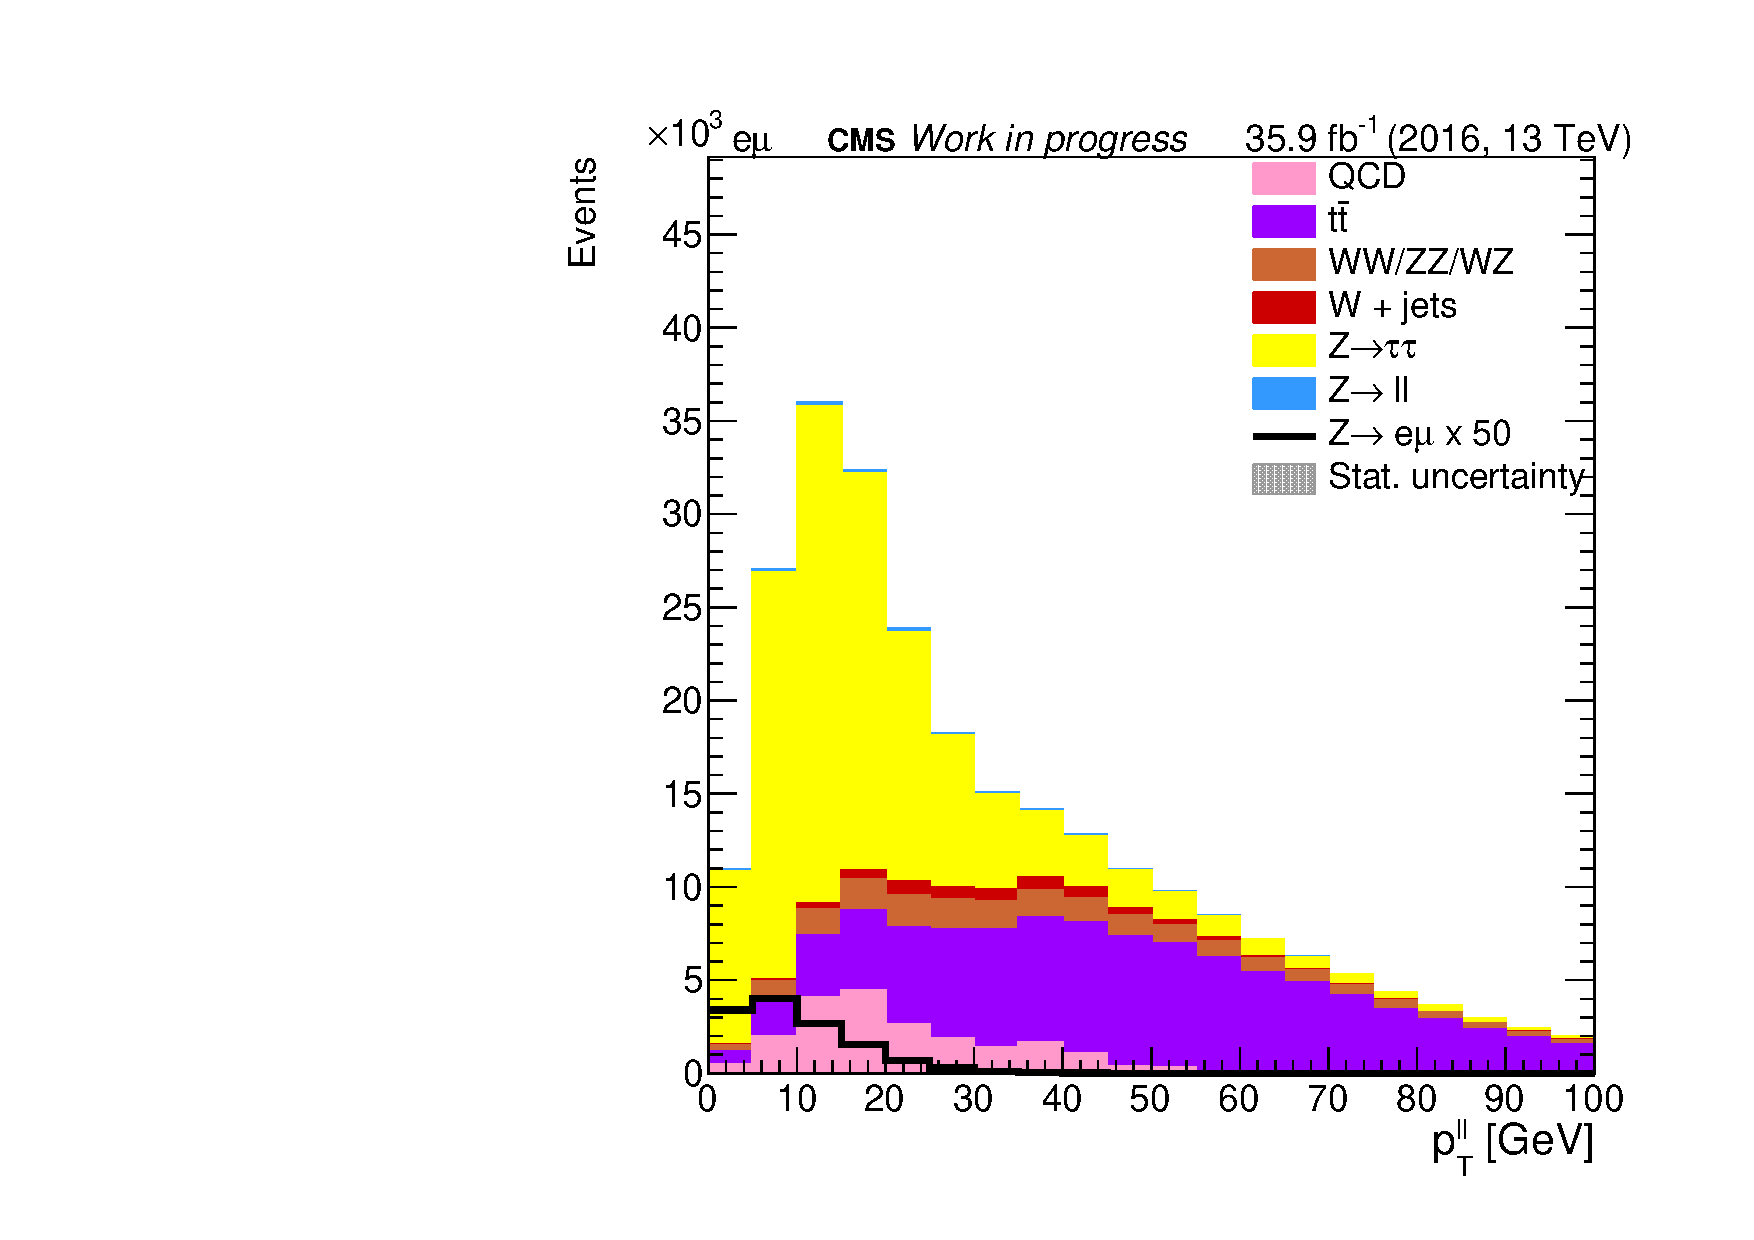
\includegraphics[width=0.45\textwidth]{plots/em/DiLepPt_withsignal.pdf}

	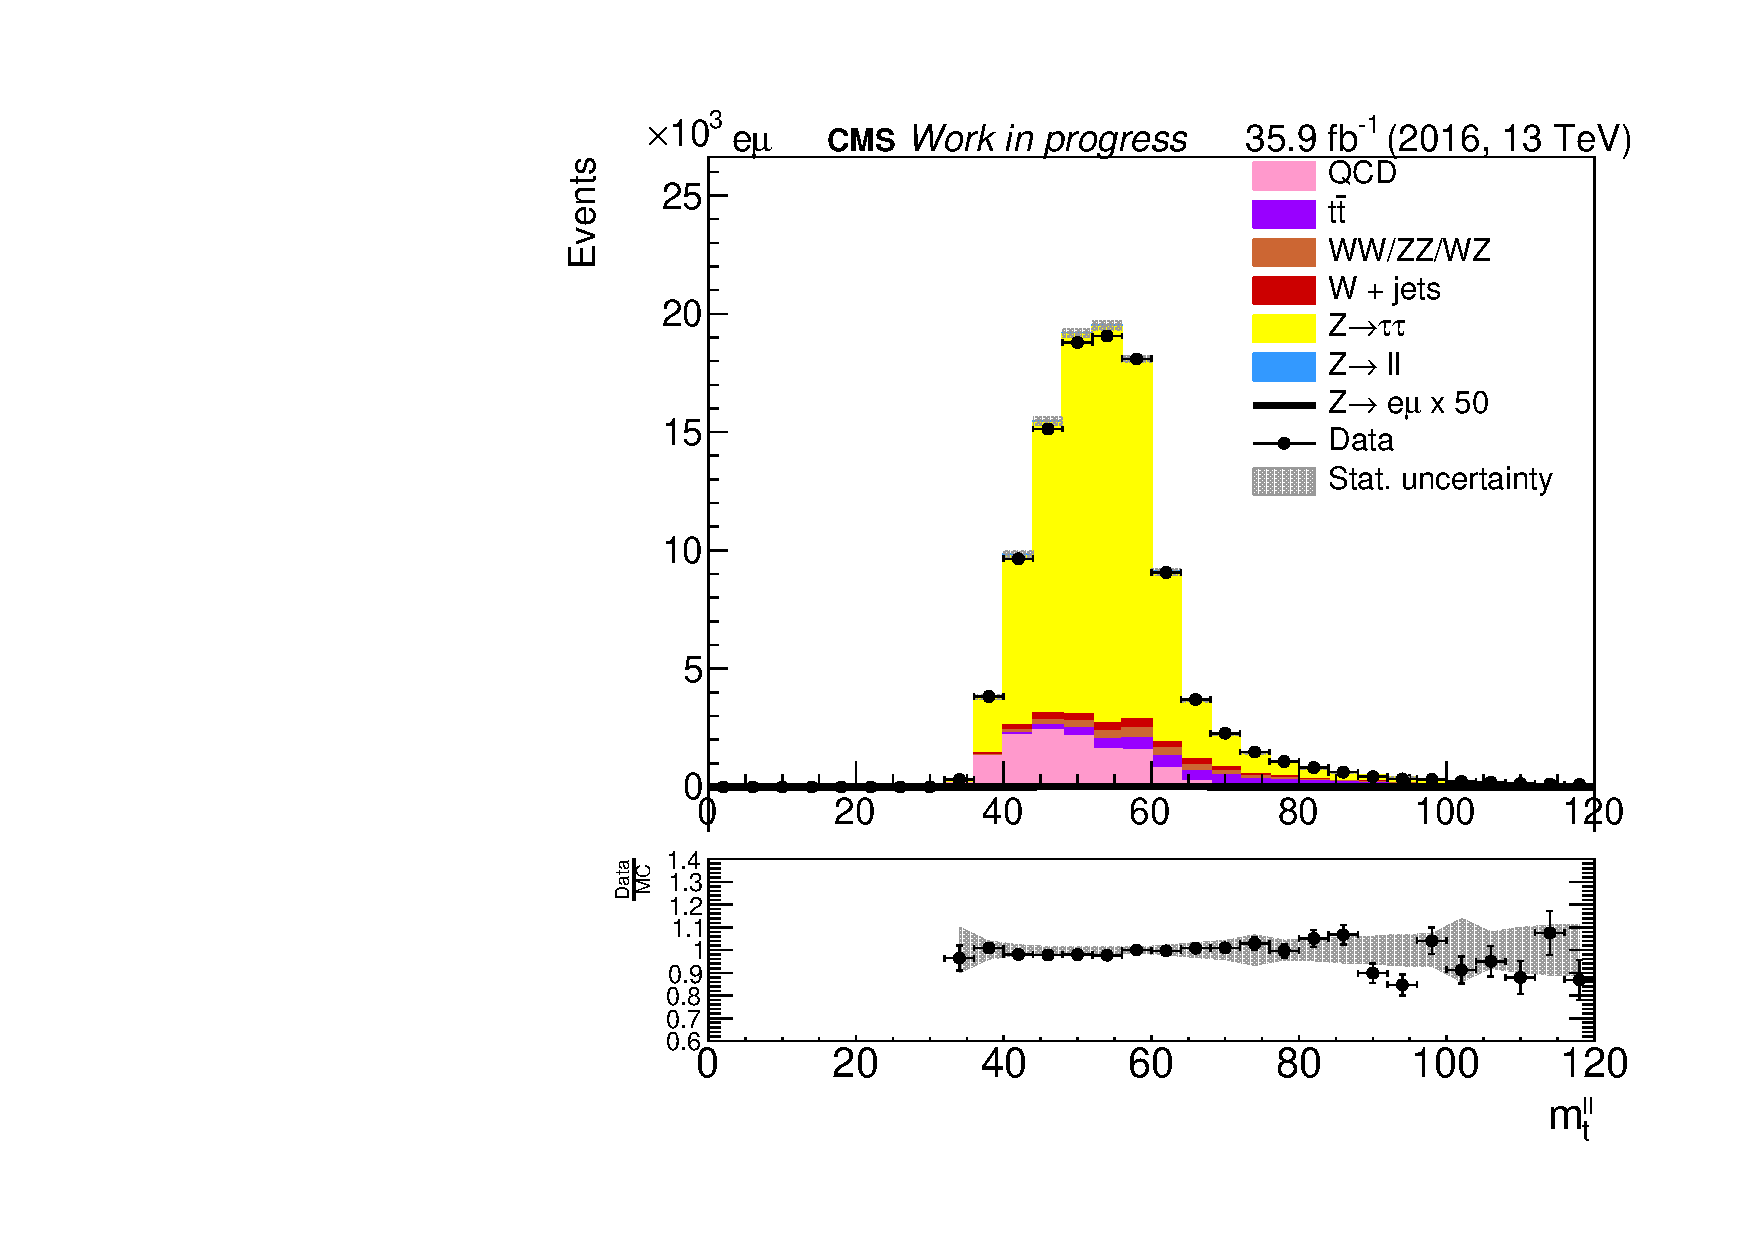
\includegraphics[width=0.45\textwidth]{plots/em/DiTransverseMass_CR.pdf}
	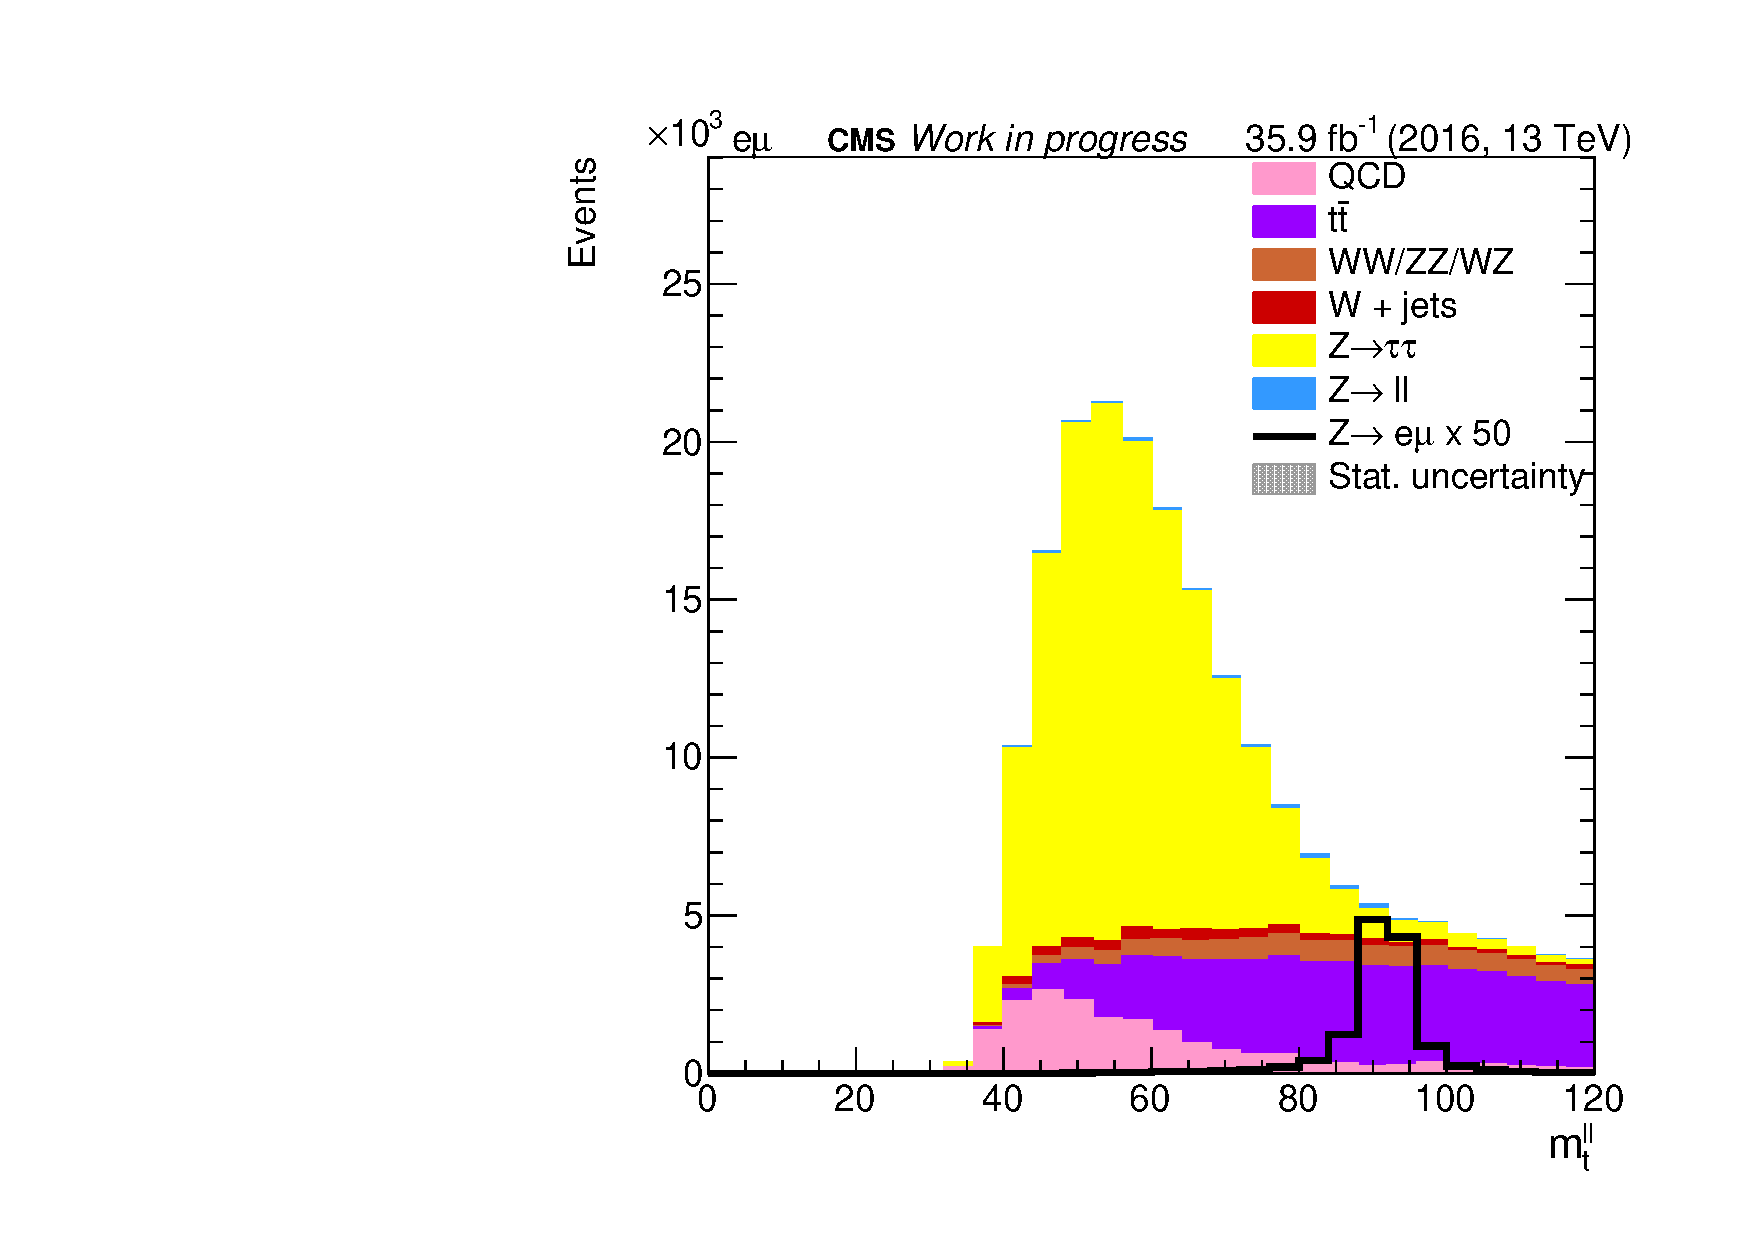
\includegraphics[width=0.45\textwidth]{plots/em/DiTransverseMass_withsignal.pdf}
\end{figure}


\begin{figure}[htp]
	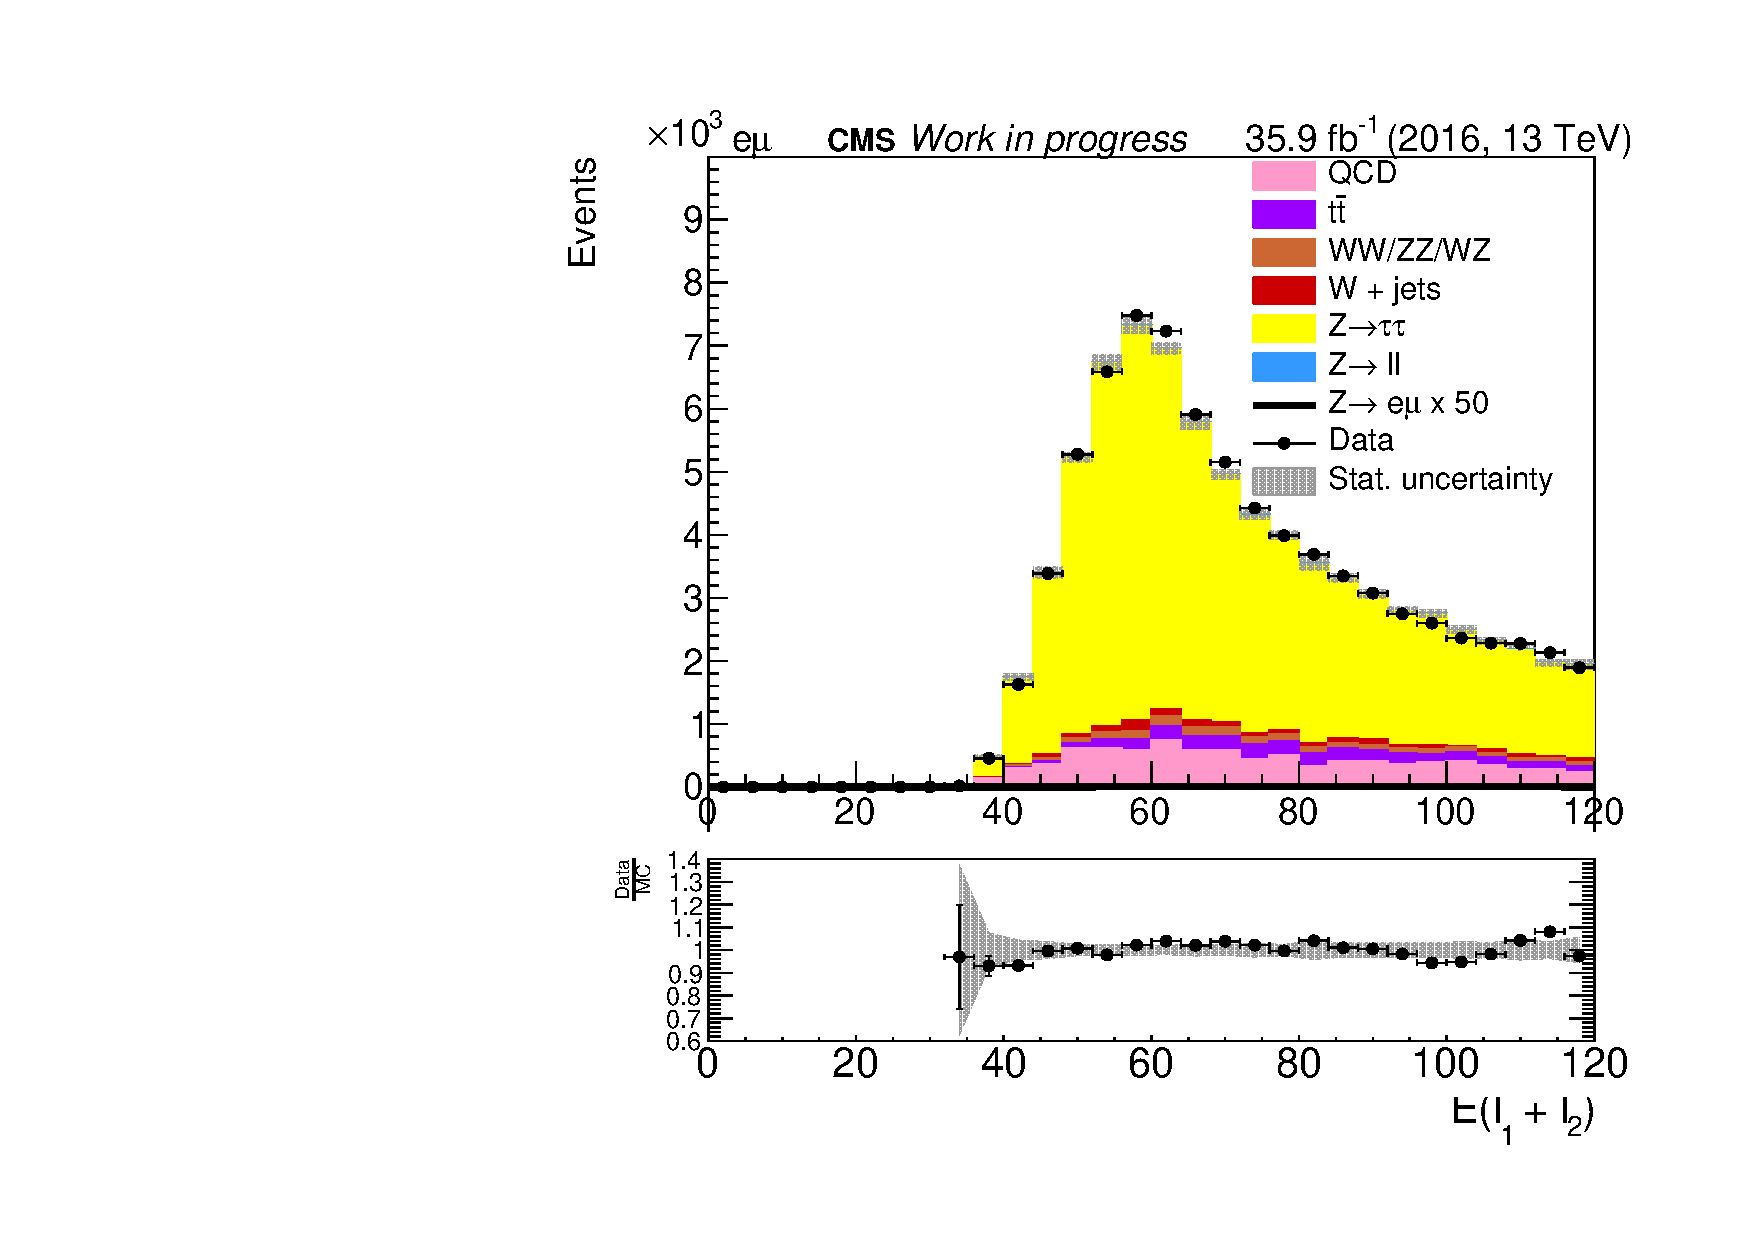
\includegraphics[width=0.45\textwidth]{plots/em/EnergySum_CR.pdf}
	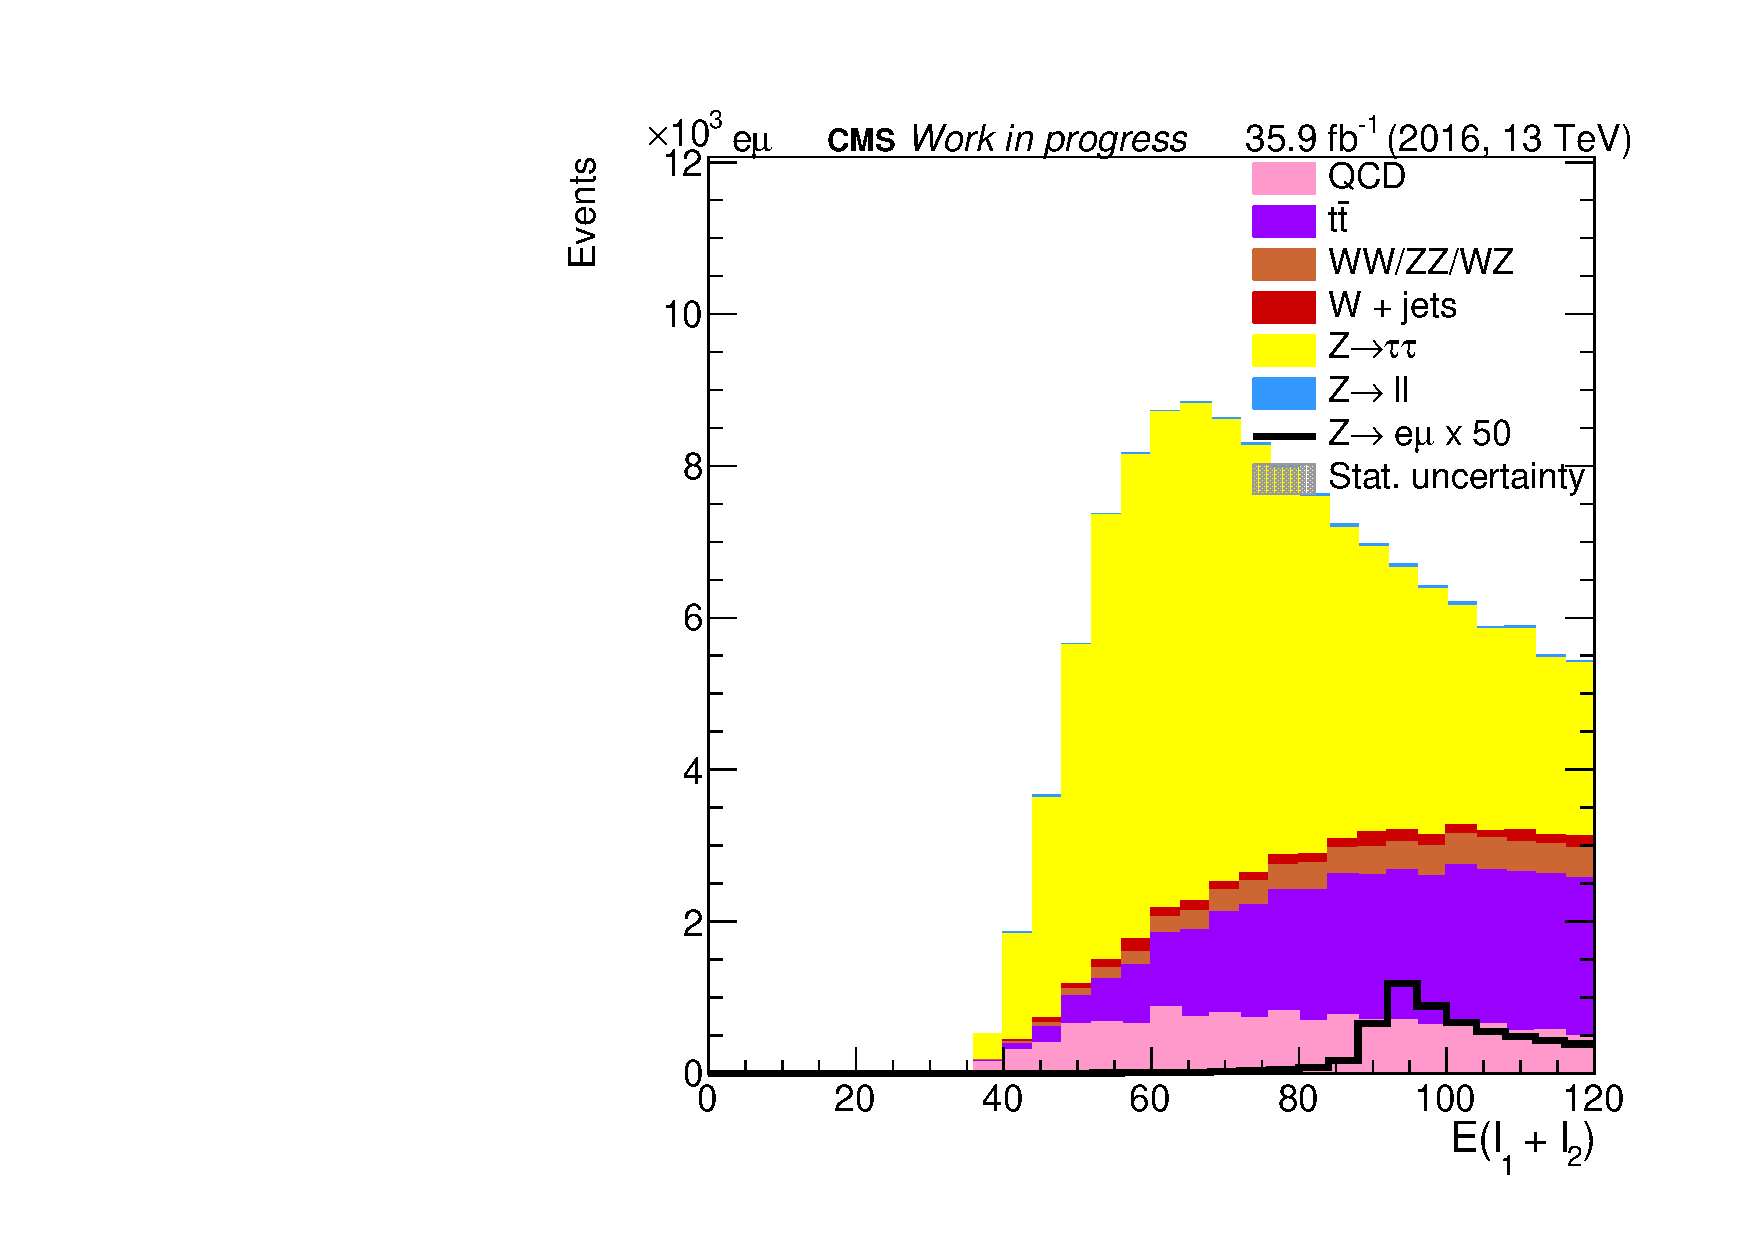
\includegraphics[width=0.45\textwidth]{plots/em/EnergySum_withsignal.pdf}

	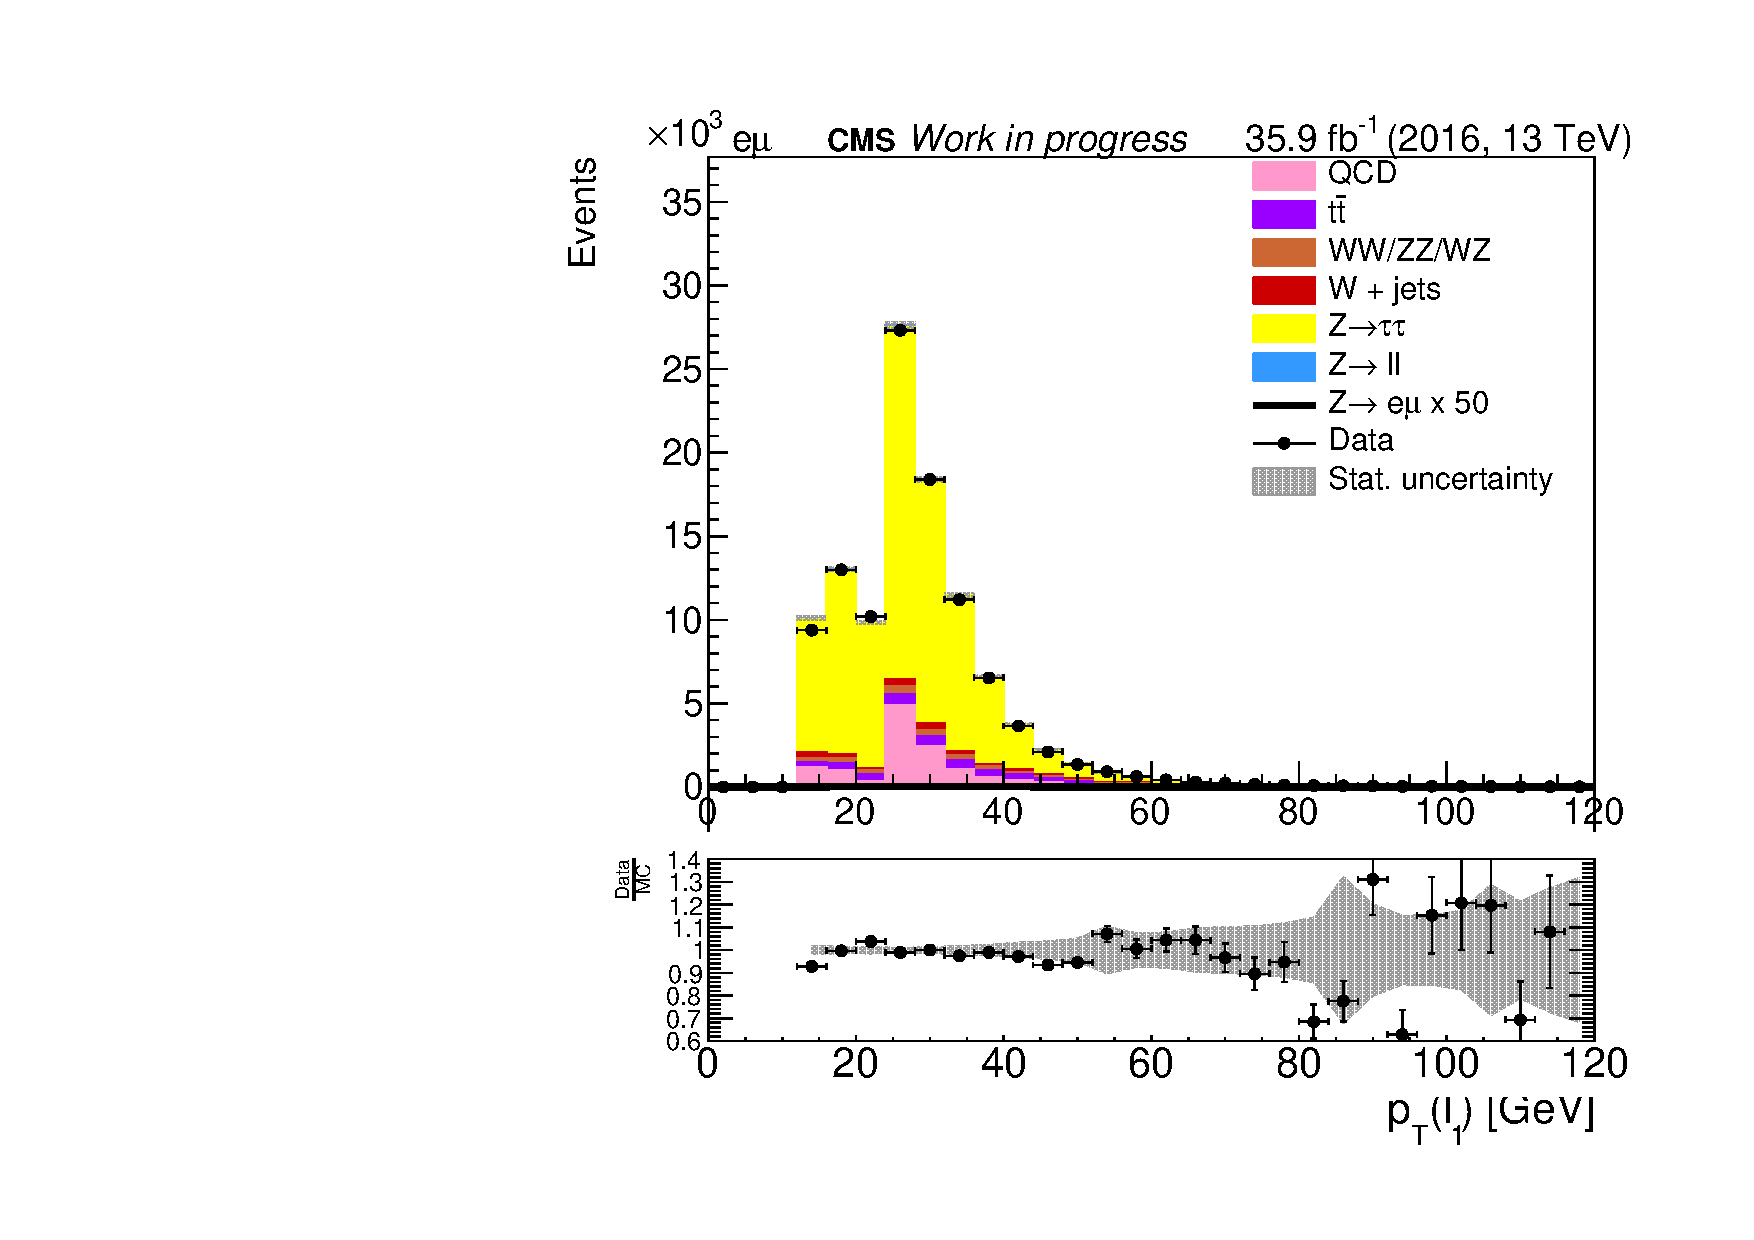
\includegraphics[width=0.45\textwidth]{plots/em/TransverseMomentum1_CR.pdf}
	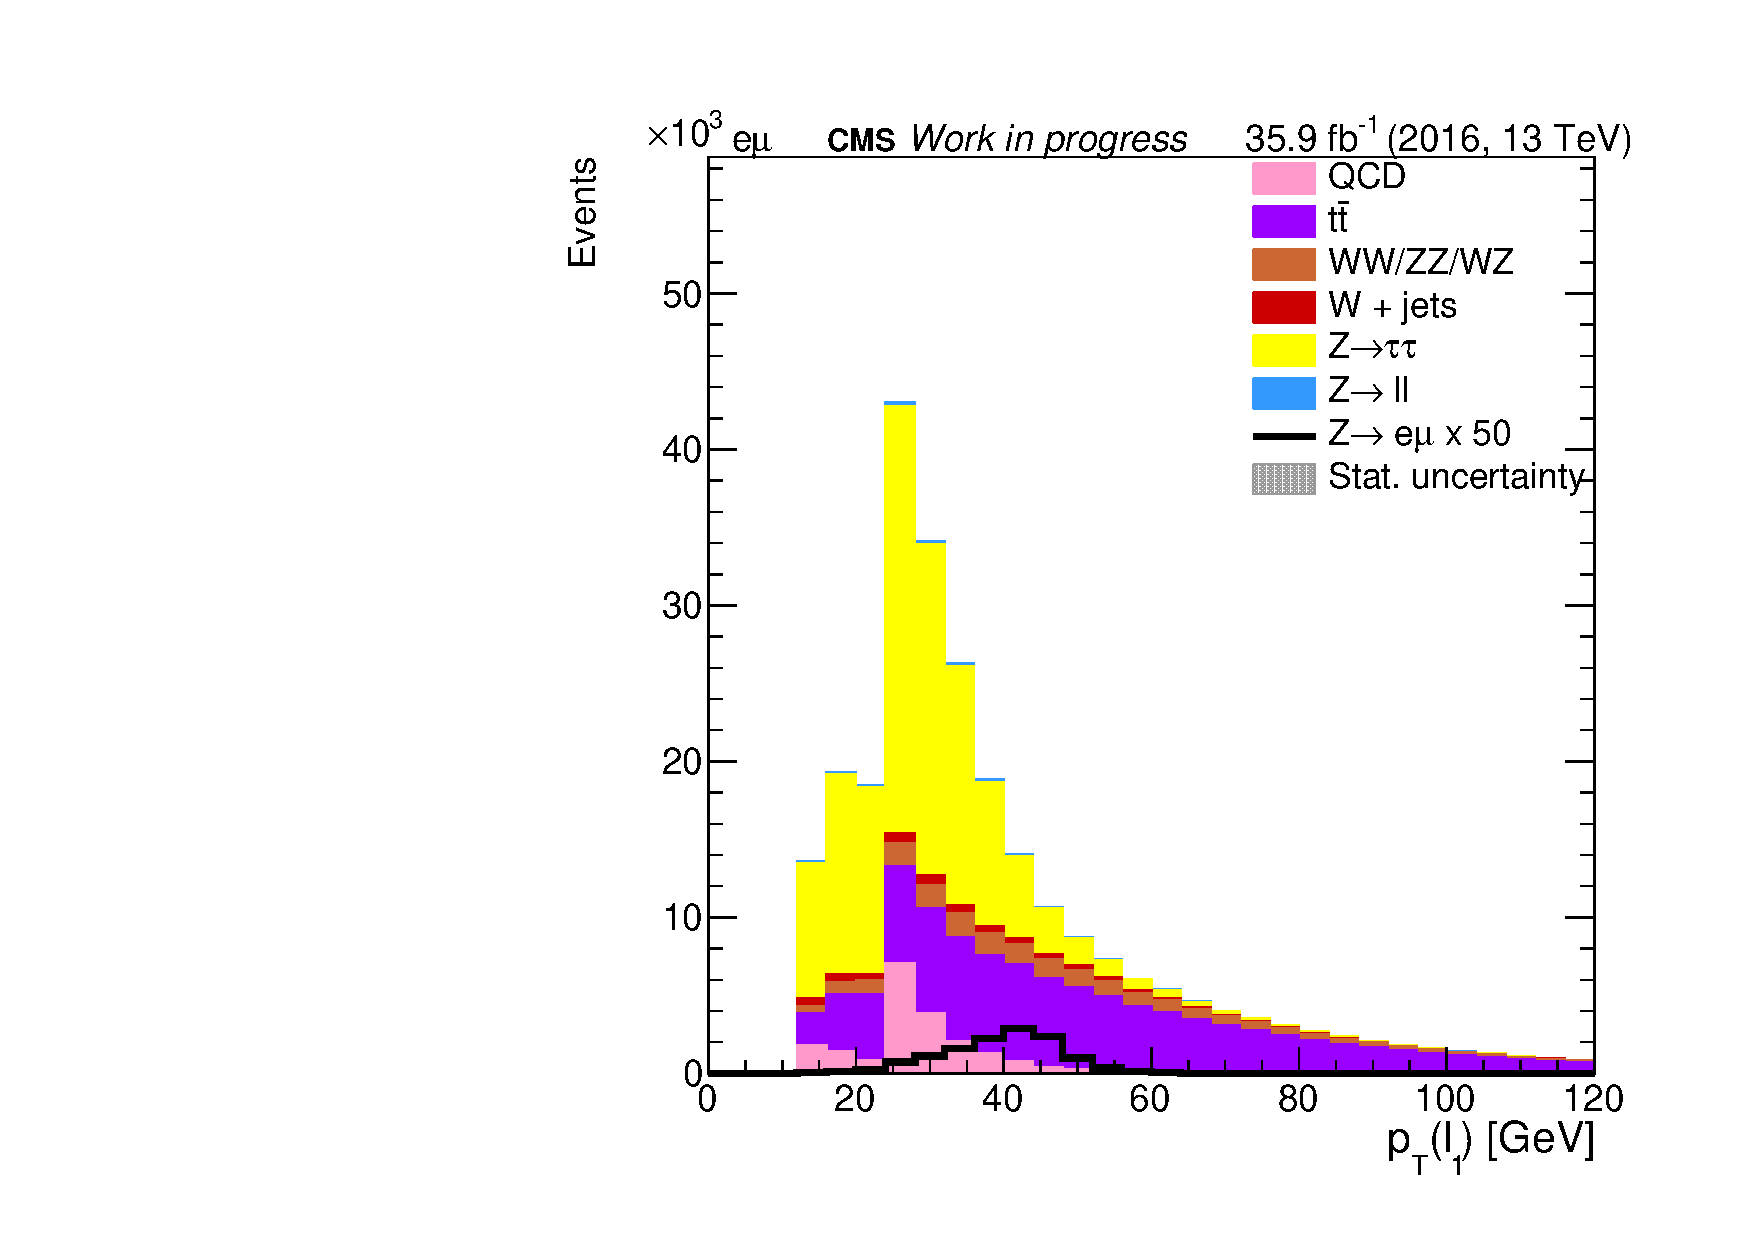
\includegraphics[width=0.45\textwidth]{plots/em/TransverseMomentum1_withsignal.pdf}

	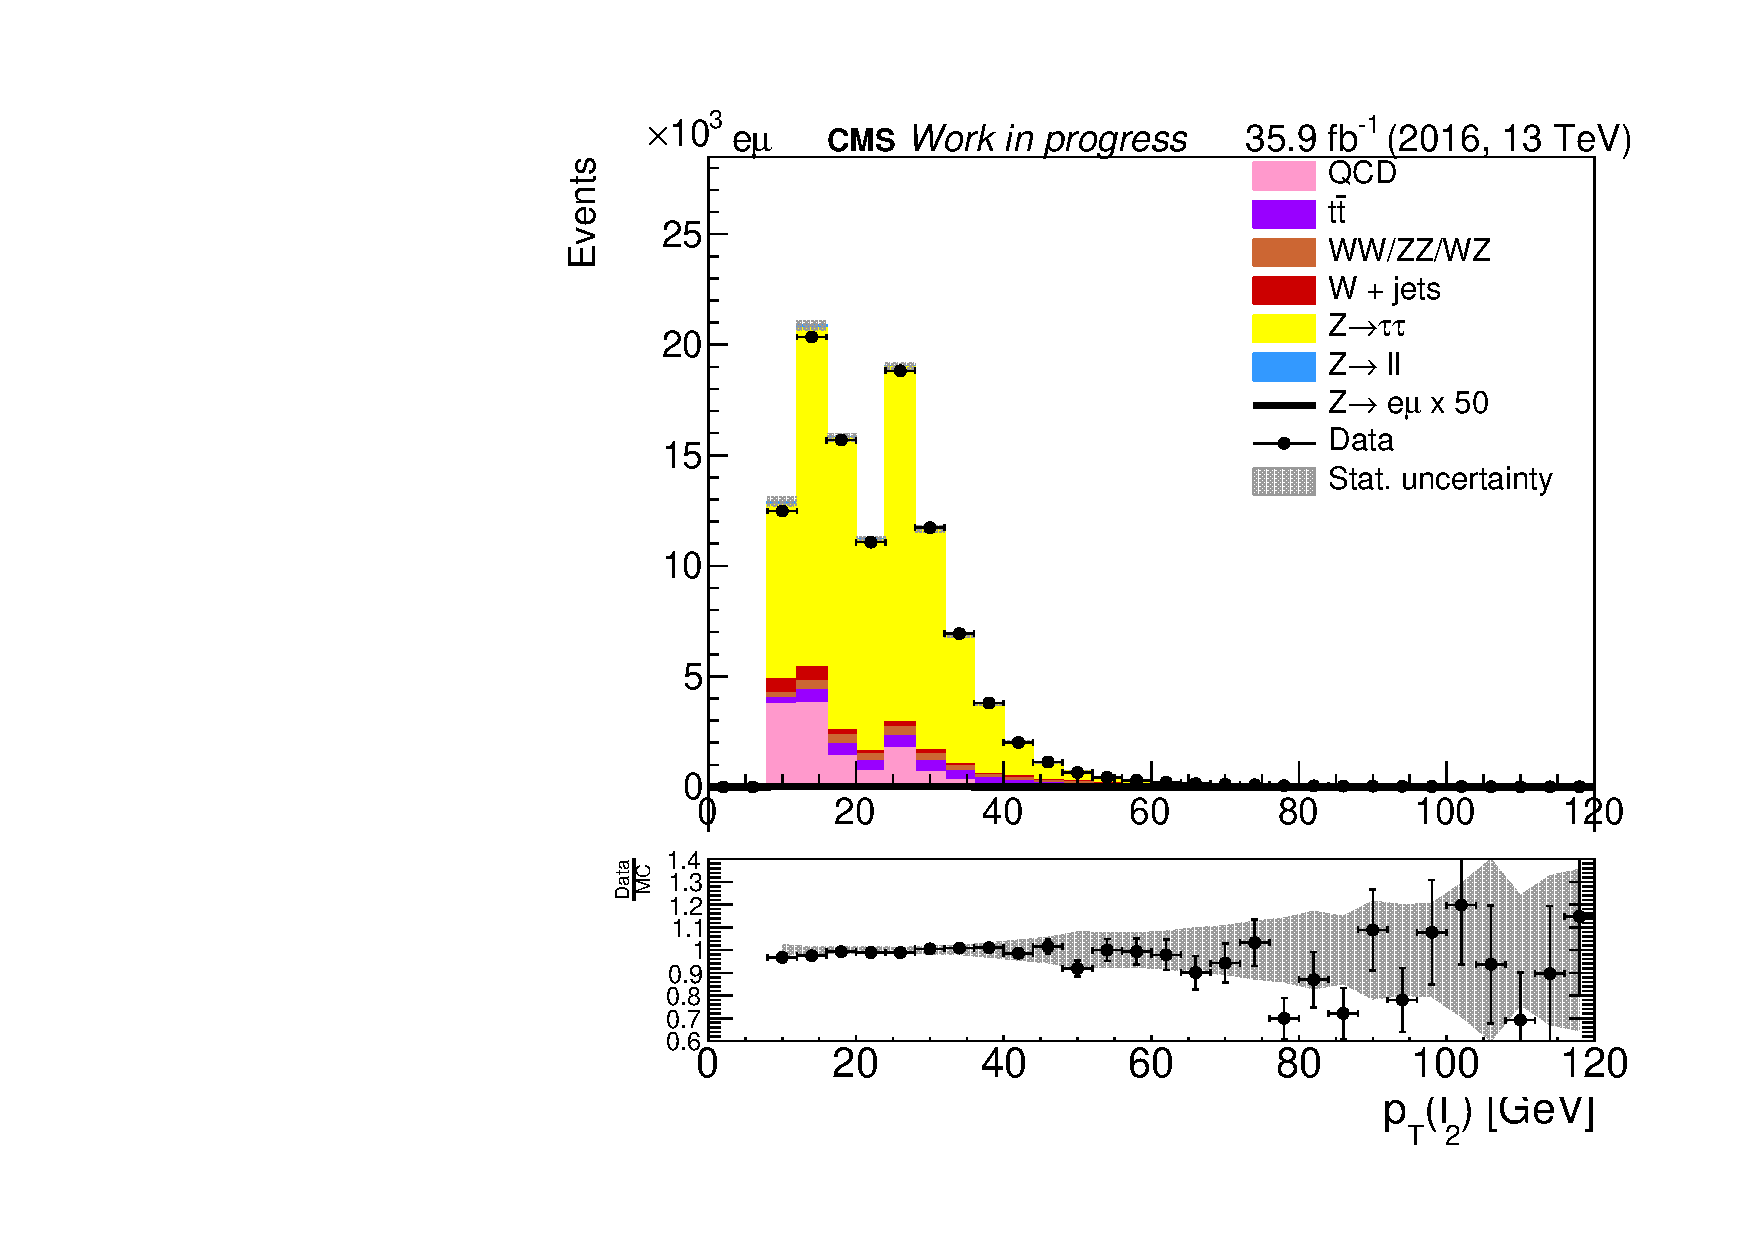
\includegraphics[width=0.45\textwidth]{plots/em/TransverseMomentum2_CR.pdf}
	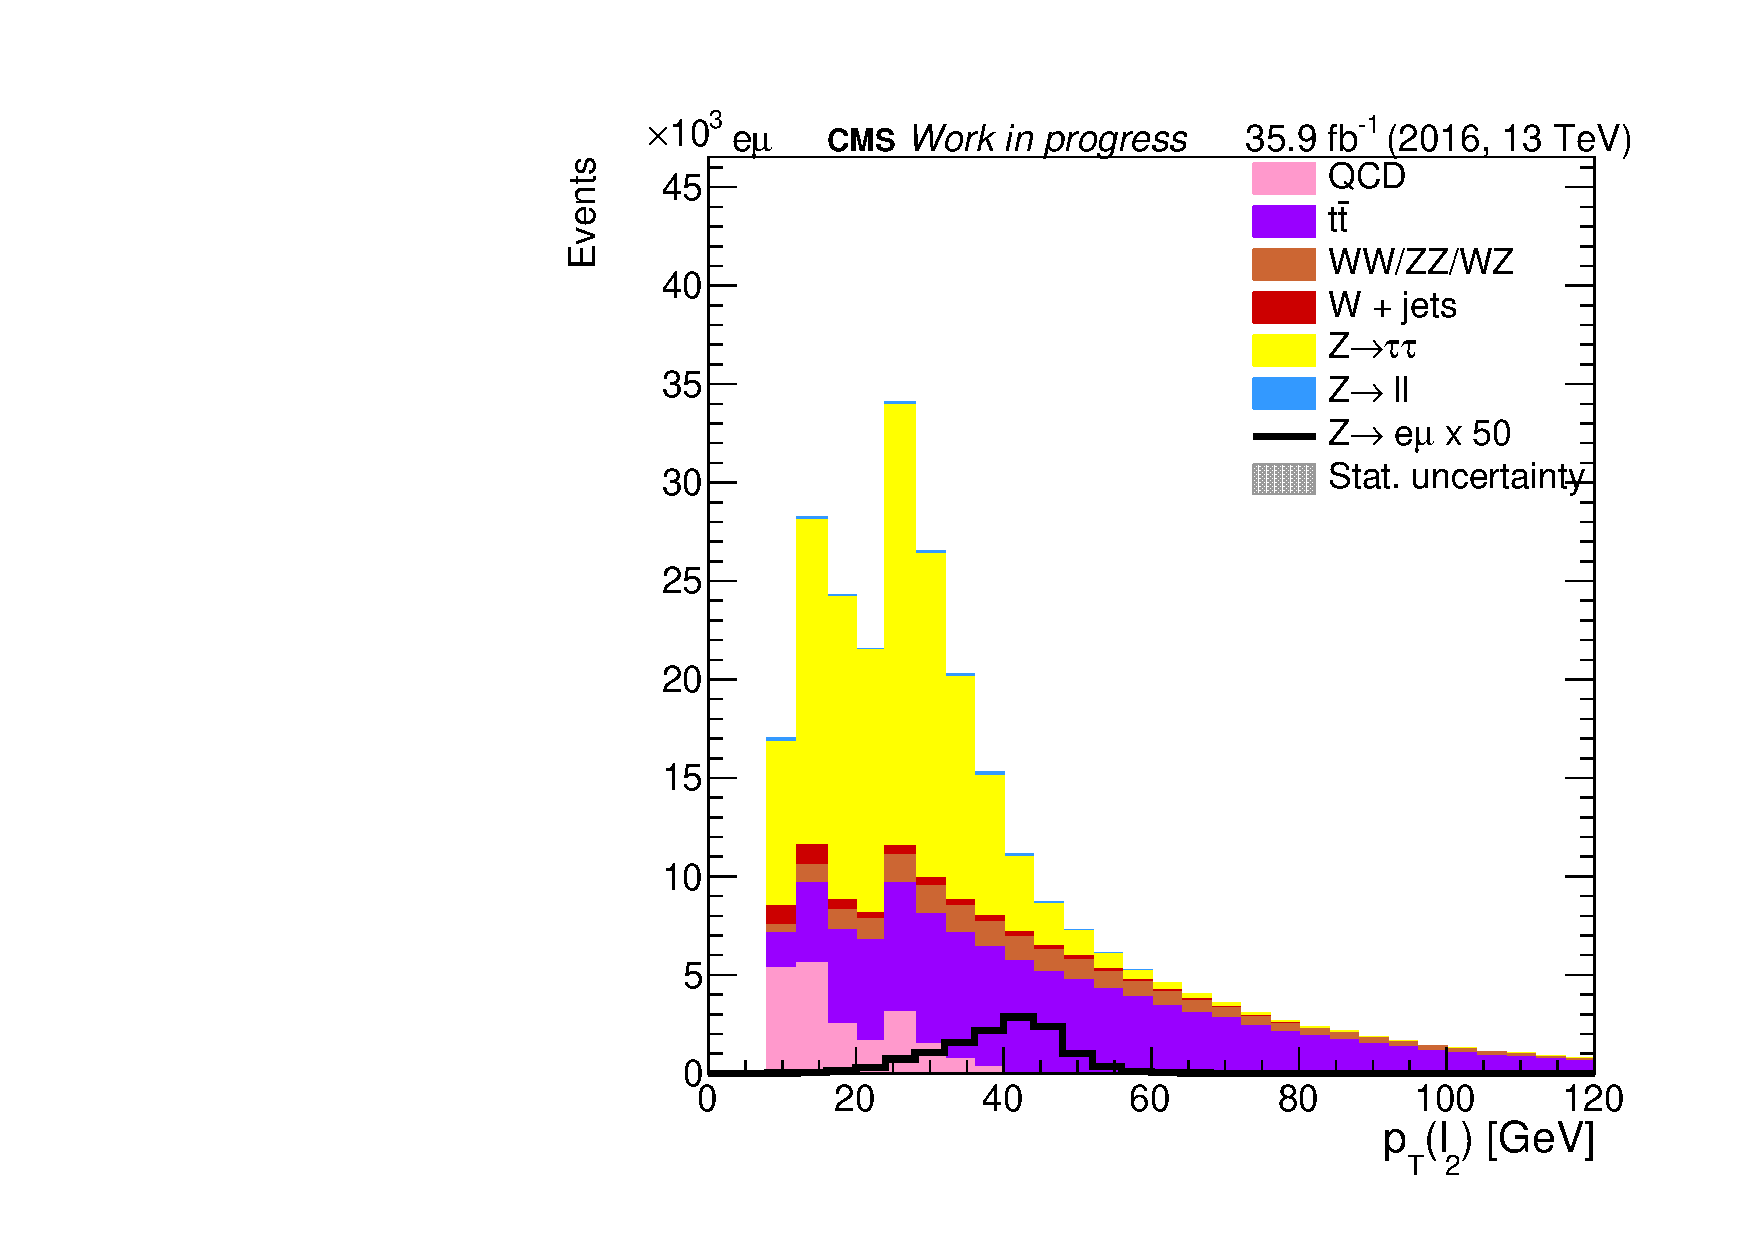
\includegraphics[width=0.45\textwidth]{plots/em/TransverseMomentum2_withsignal.pdf}
\end{figure}


\begin{figure}[htp]
	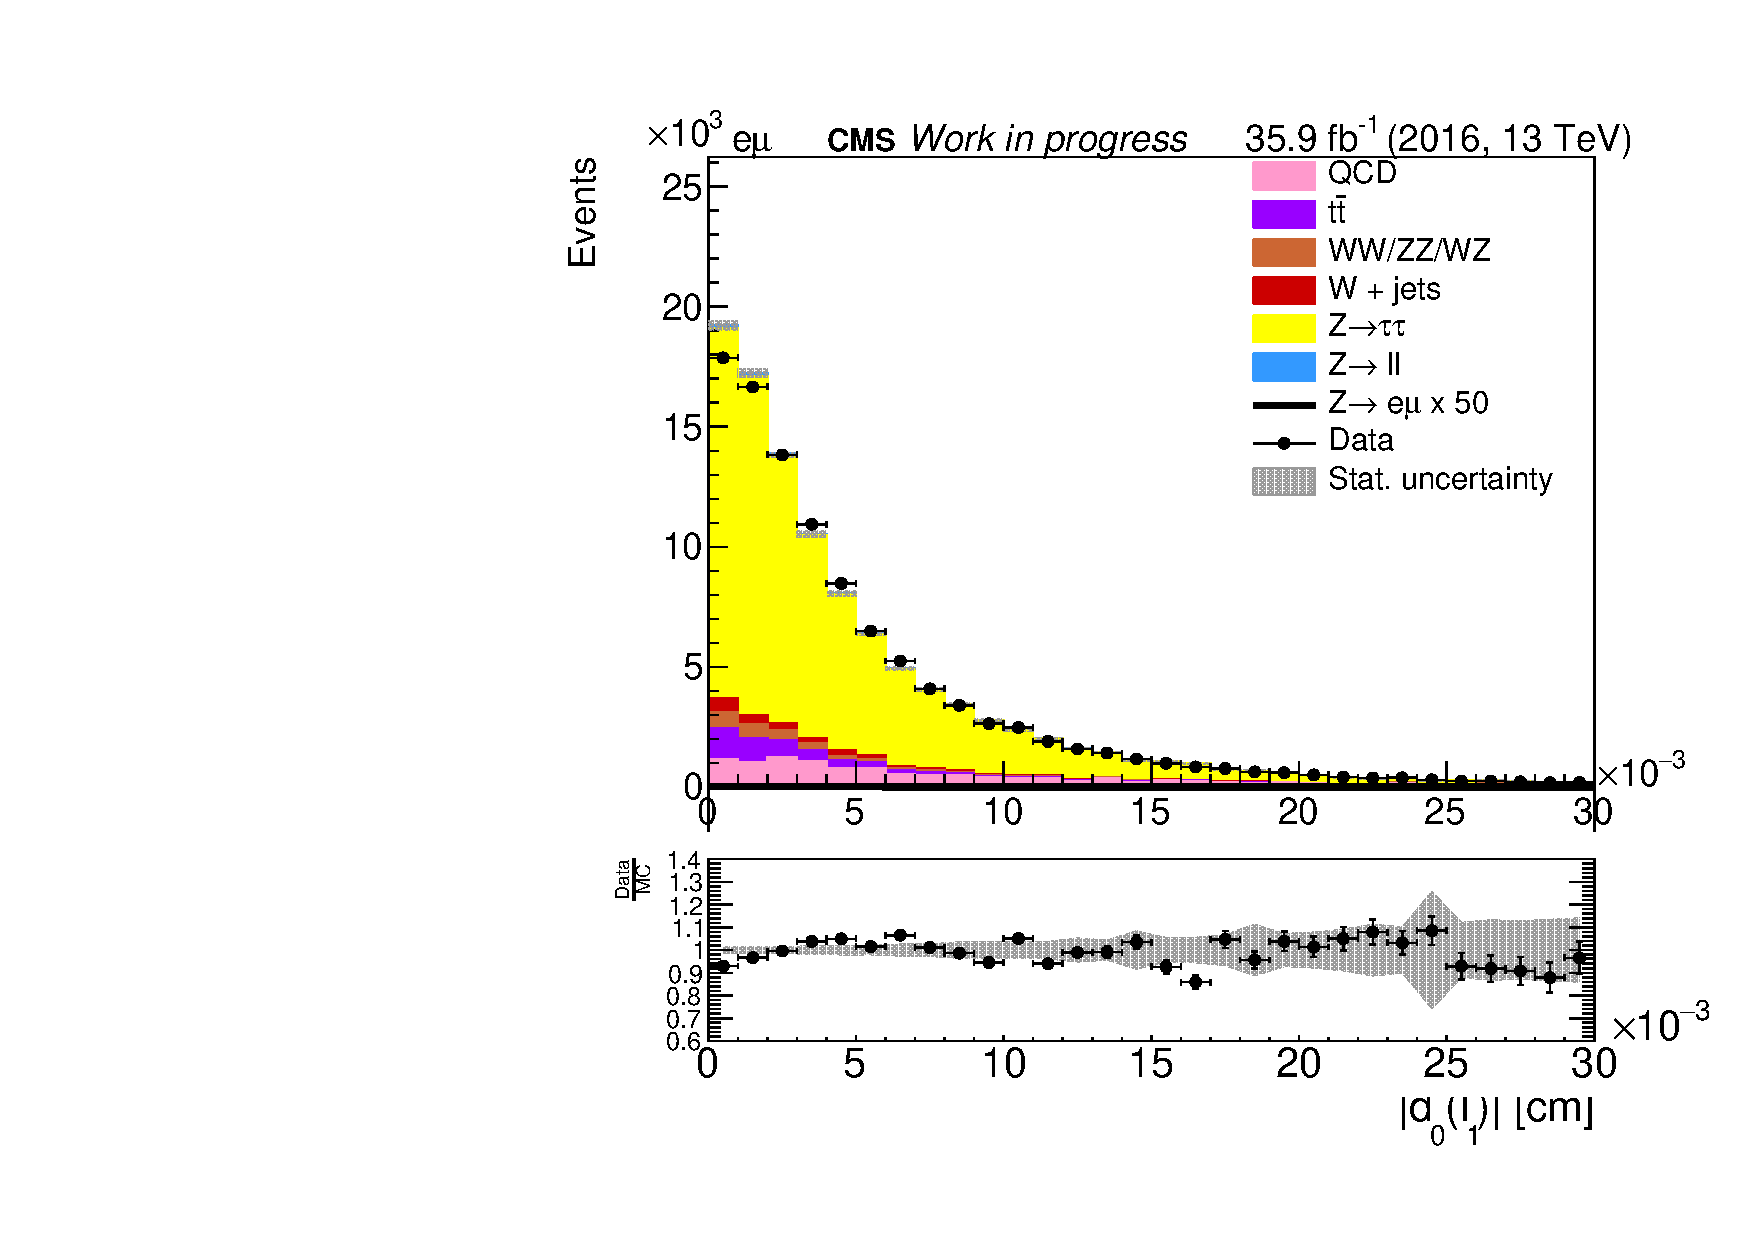
\includegraphics[width=0.45\textwidth]{plots/em/ImpactParameter1_CR.pdf}
	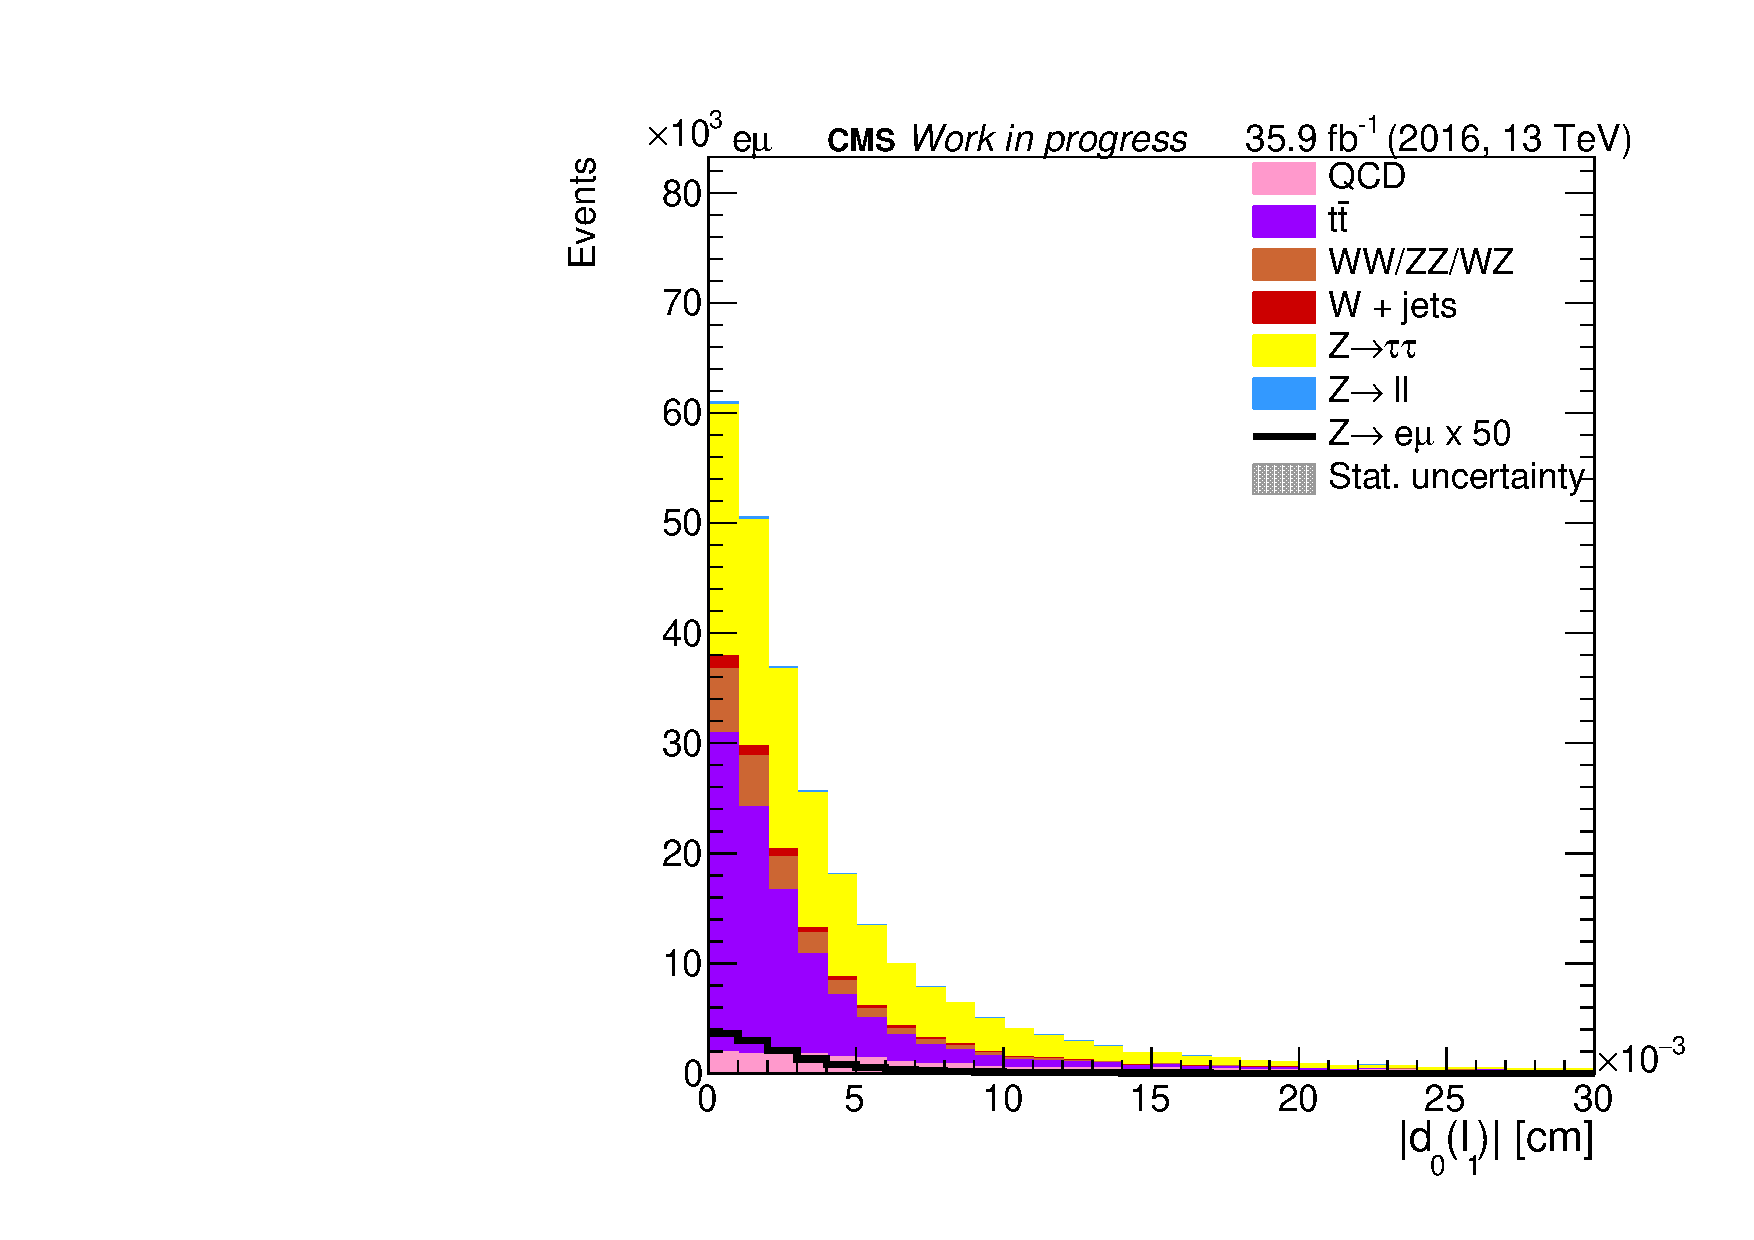
\includegraphics[width=0.45\textwidth]{plots/em/ImpactParameter1_withsignal.pdf}

	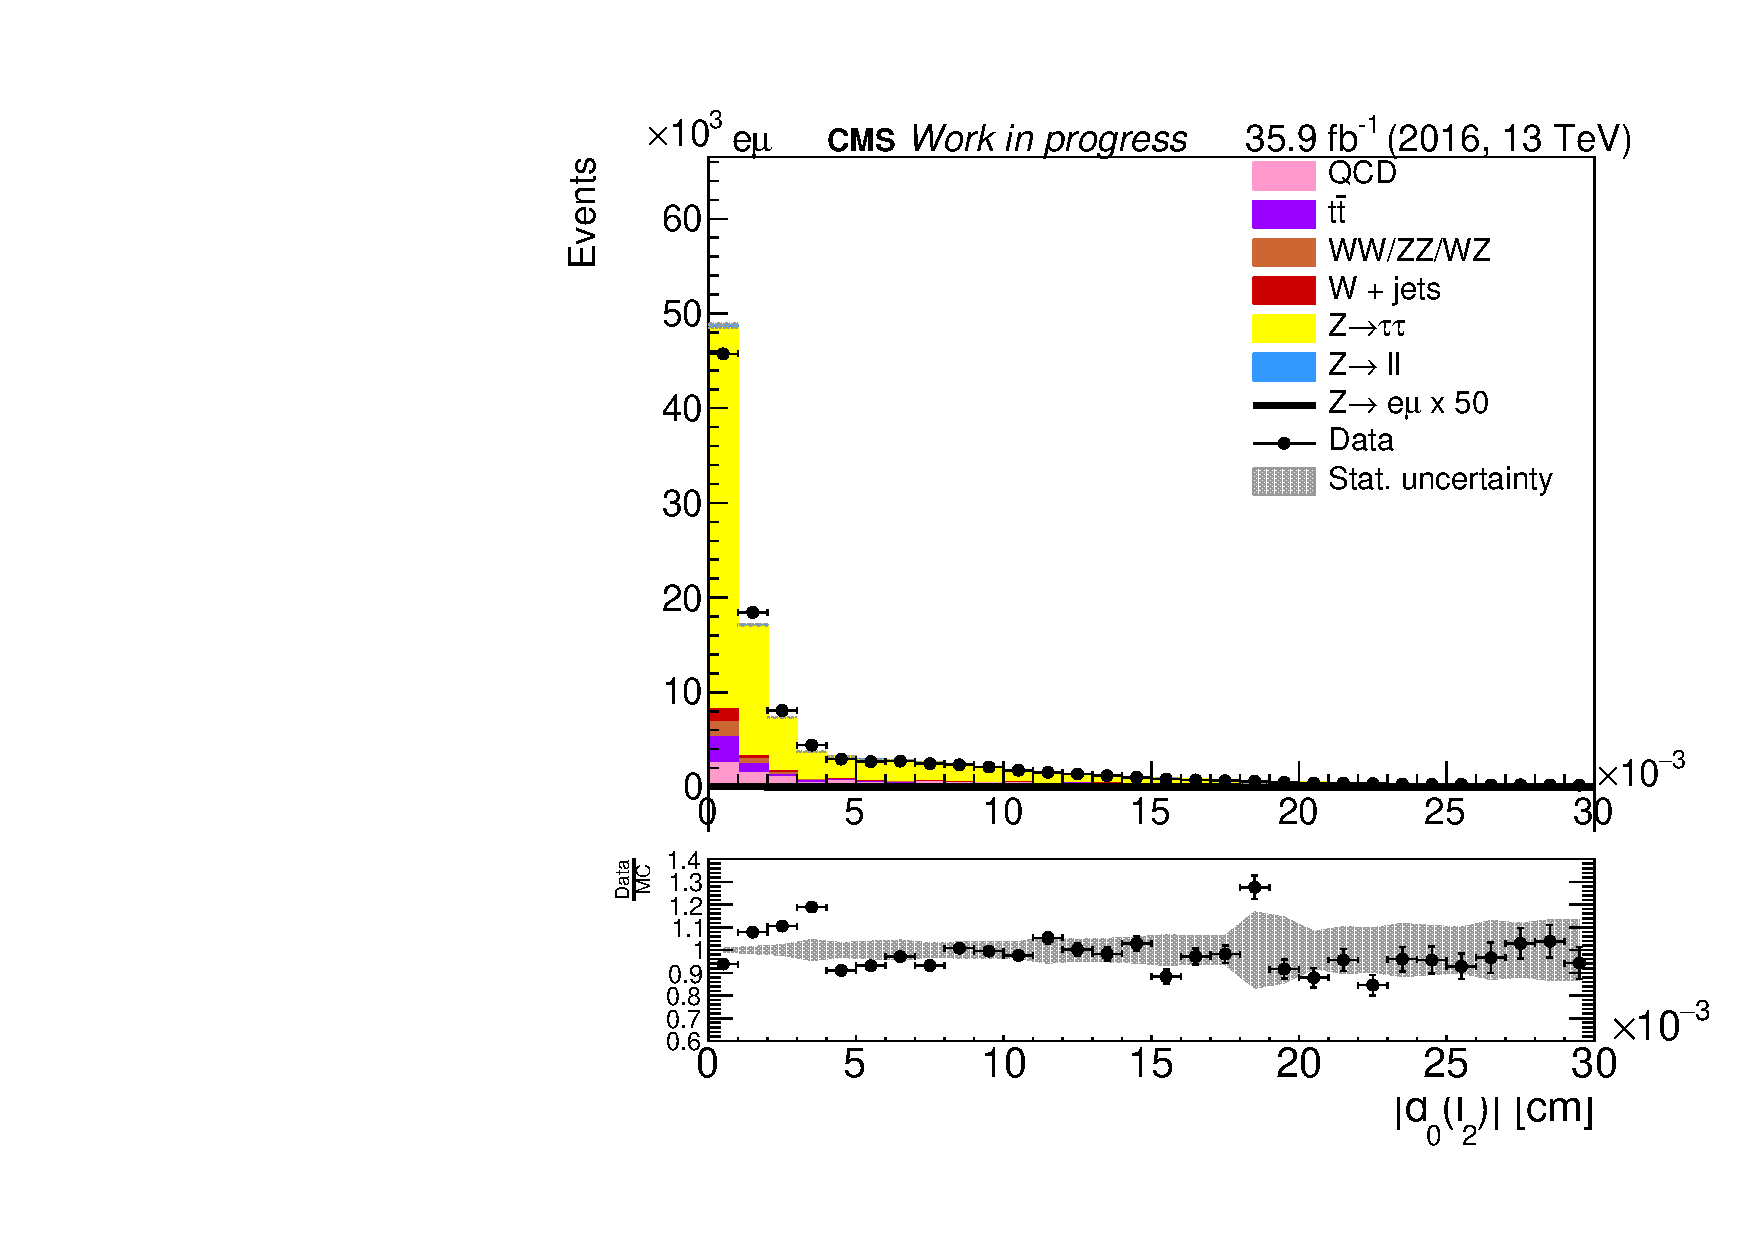
\includegraphics[width=0.45\textwidth]{plots/em/ImpactParameter2_CR.pdf}
	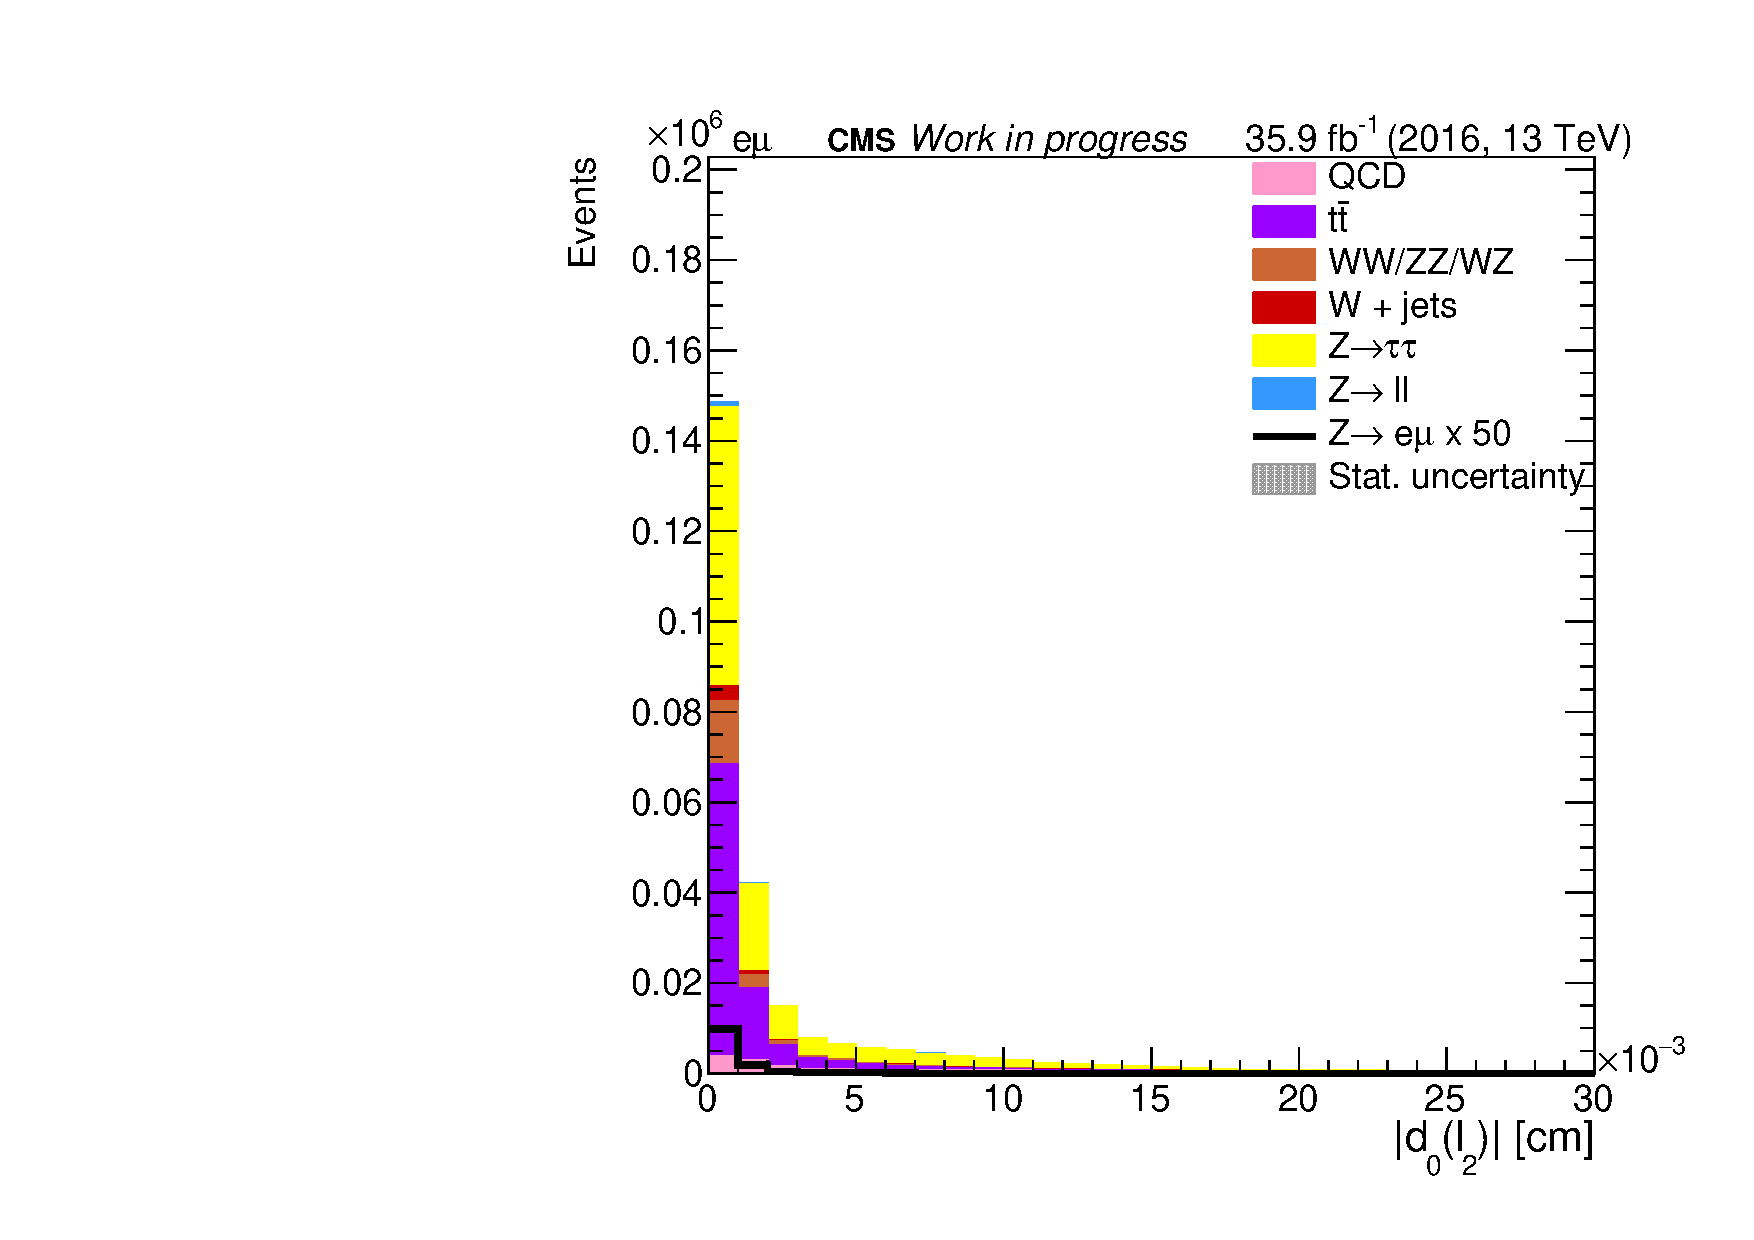
\includegraphics[width=0.45\textwidth]{plots/em/ImpactParameter2_withsignal.pdf}

	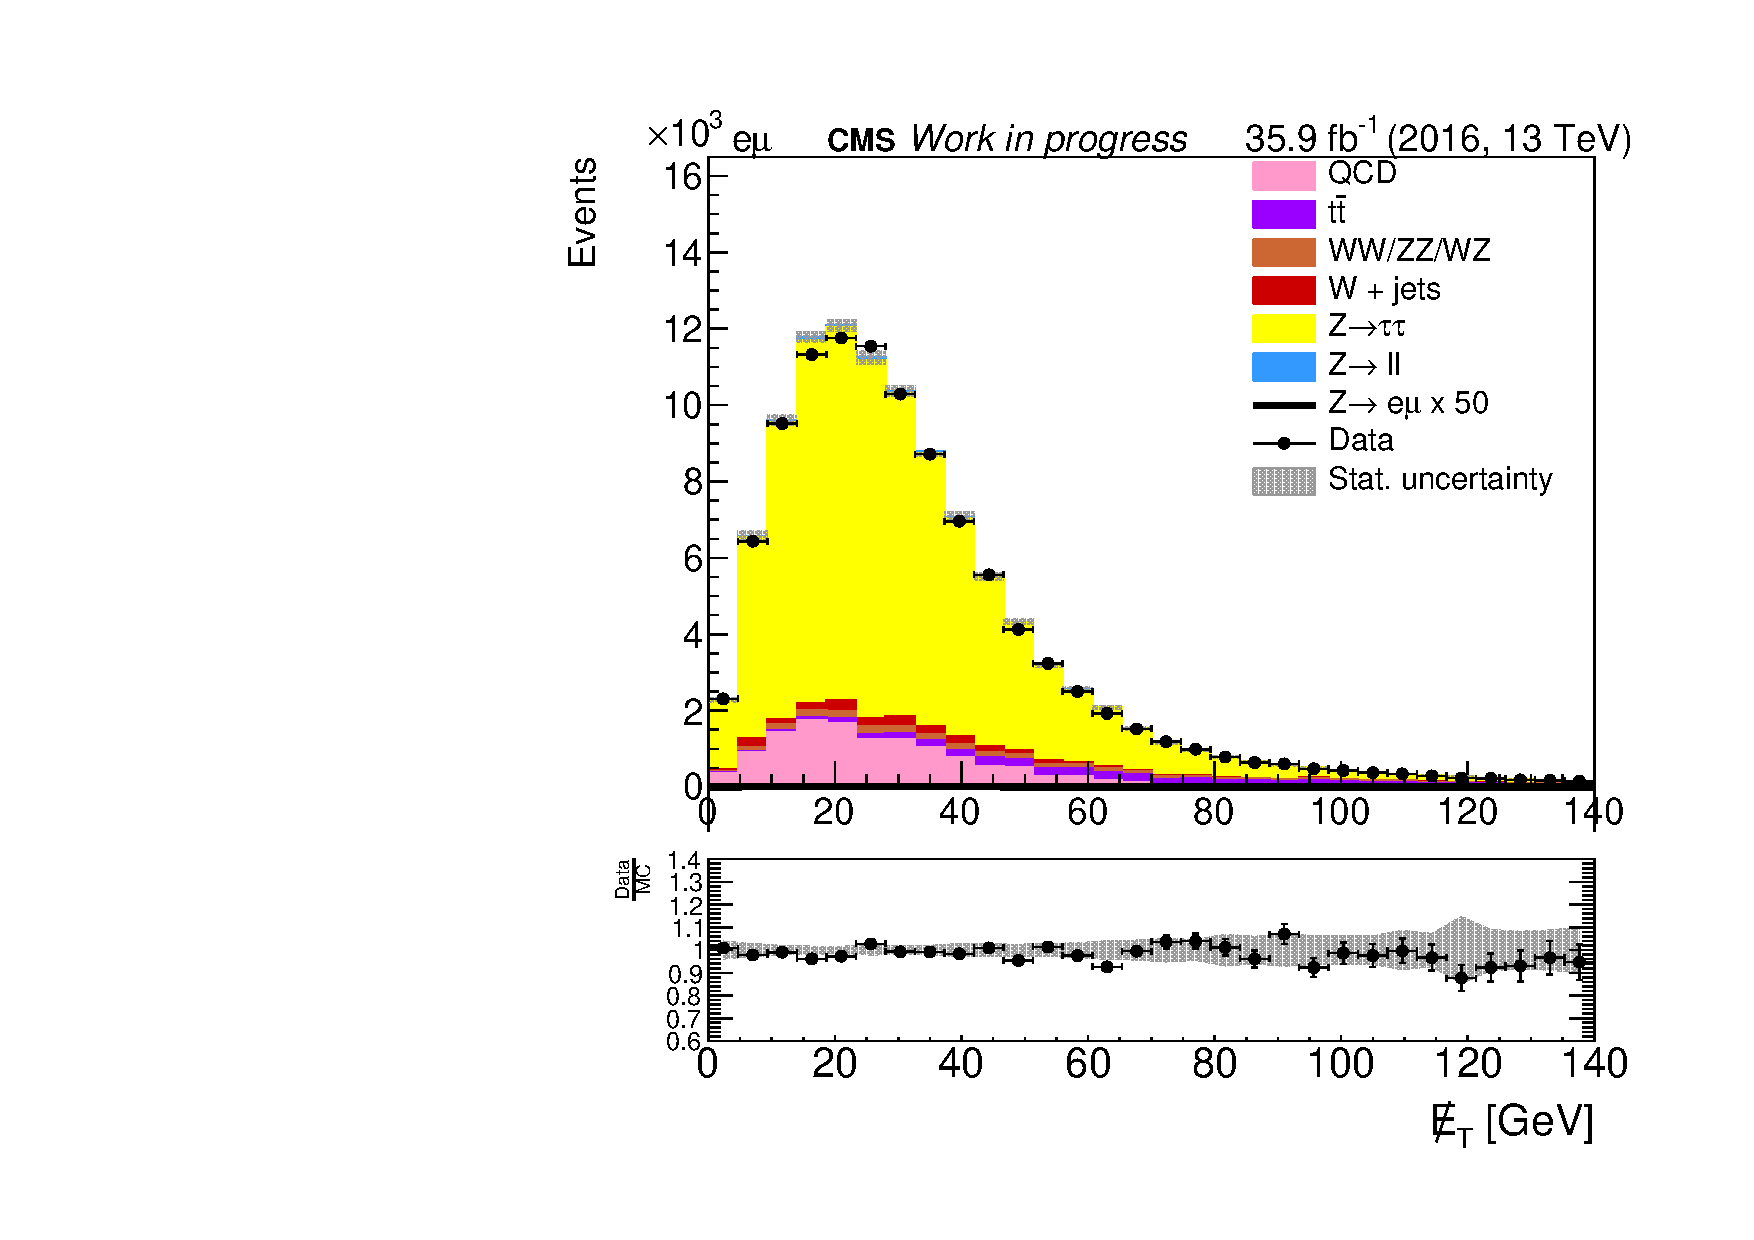
\includegraphics[width=0.45\textwidth]{plots/em/MissingTranverseEnergy_CR.pdf}
	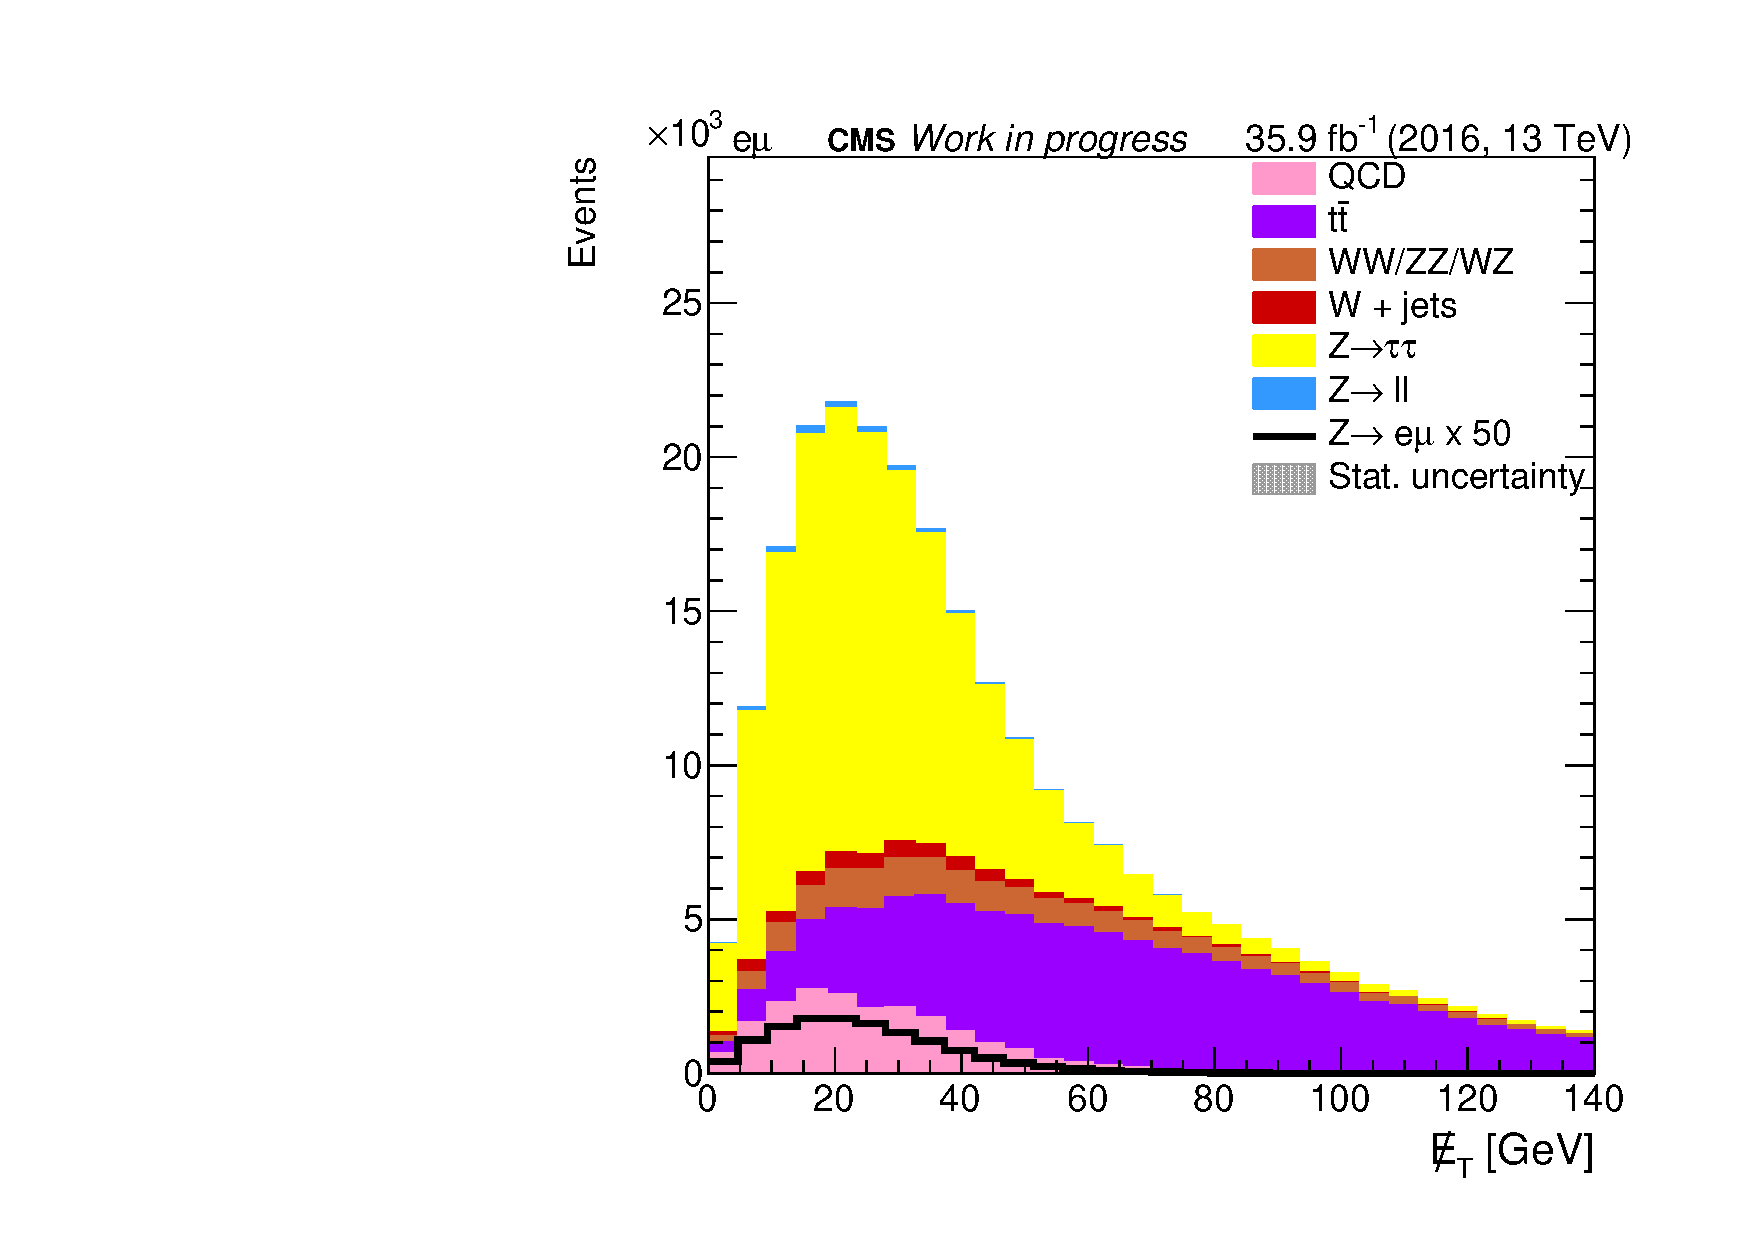
\includegraphics[width=0.45\textwidth]{plots/em/MissingTranverseEnergy_withsignal.pdf}
\end{figure}

\newpage

\section*{Plot for the $e\tau$ final state}

\begin{figure}[htp]
	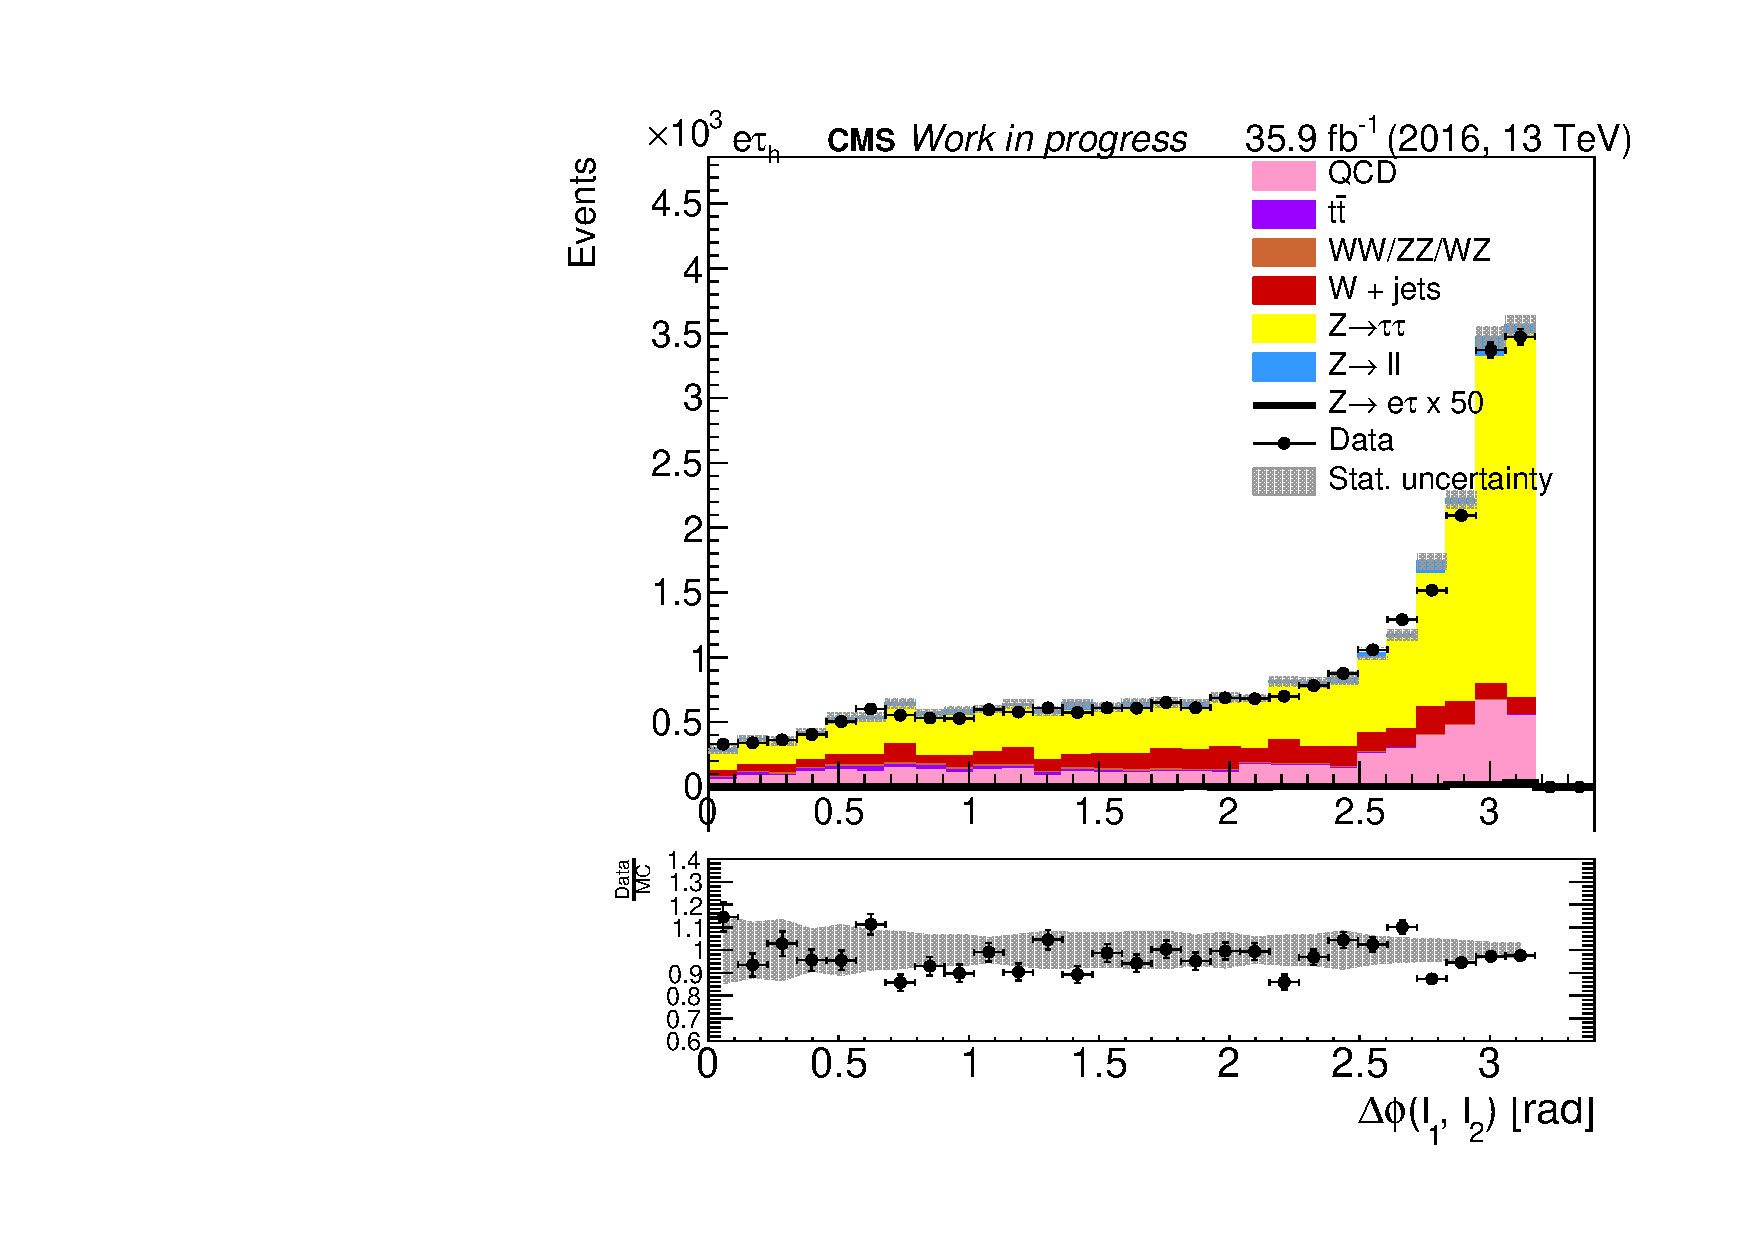
\includegraphics[width=0.45\textwidth]{plots/et/DeltaPhiL1L2_CR.pdf}
	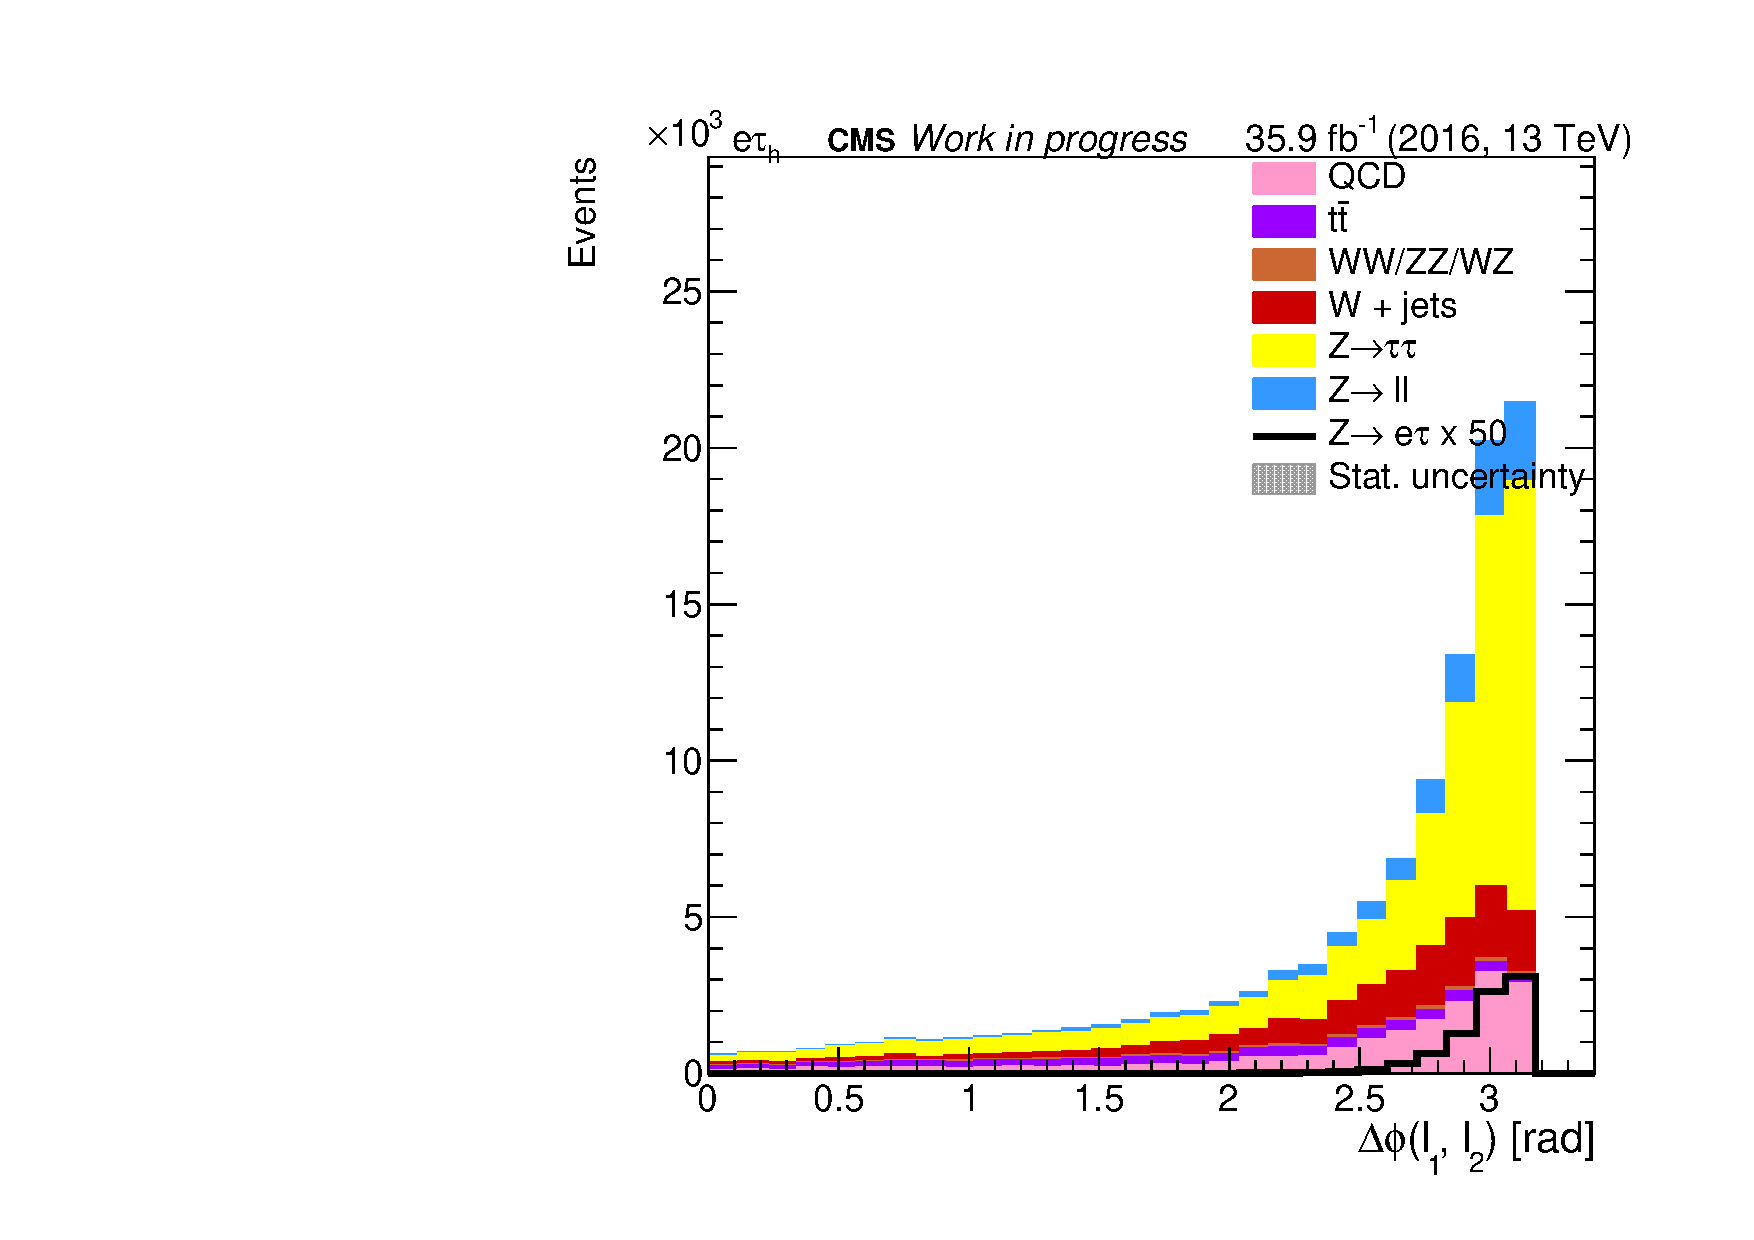
\includegraphics[width=0.45\textwidth]{plots/et/DeltaPhiL1L2_withsignal.pdf}

	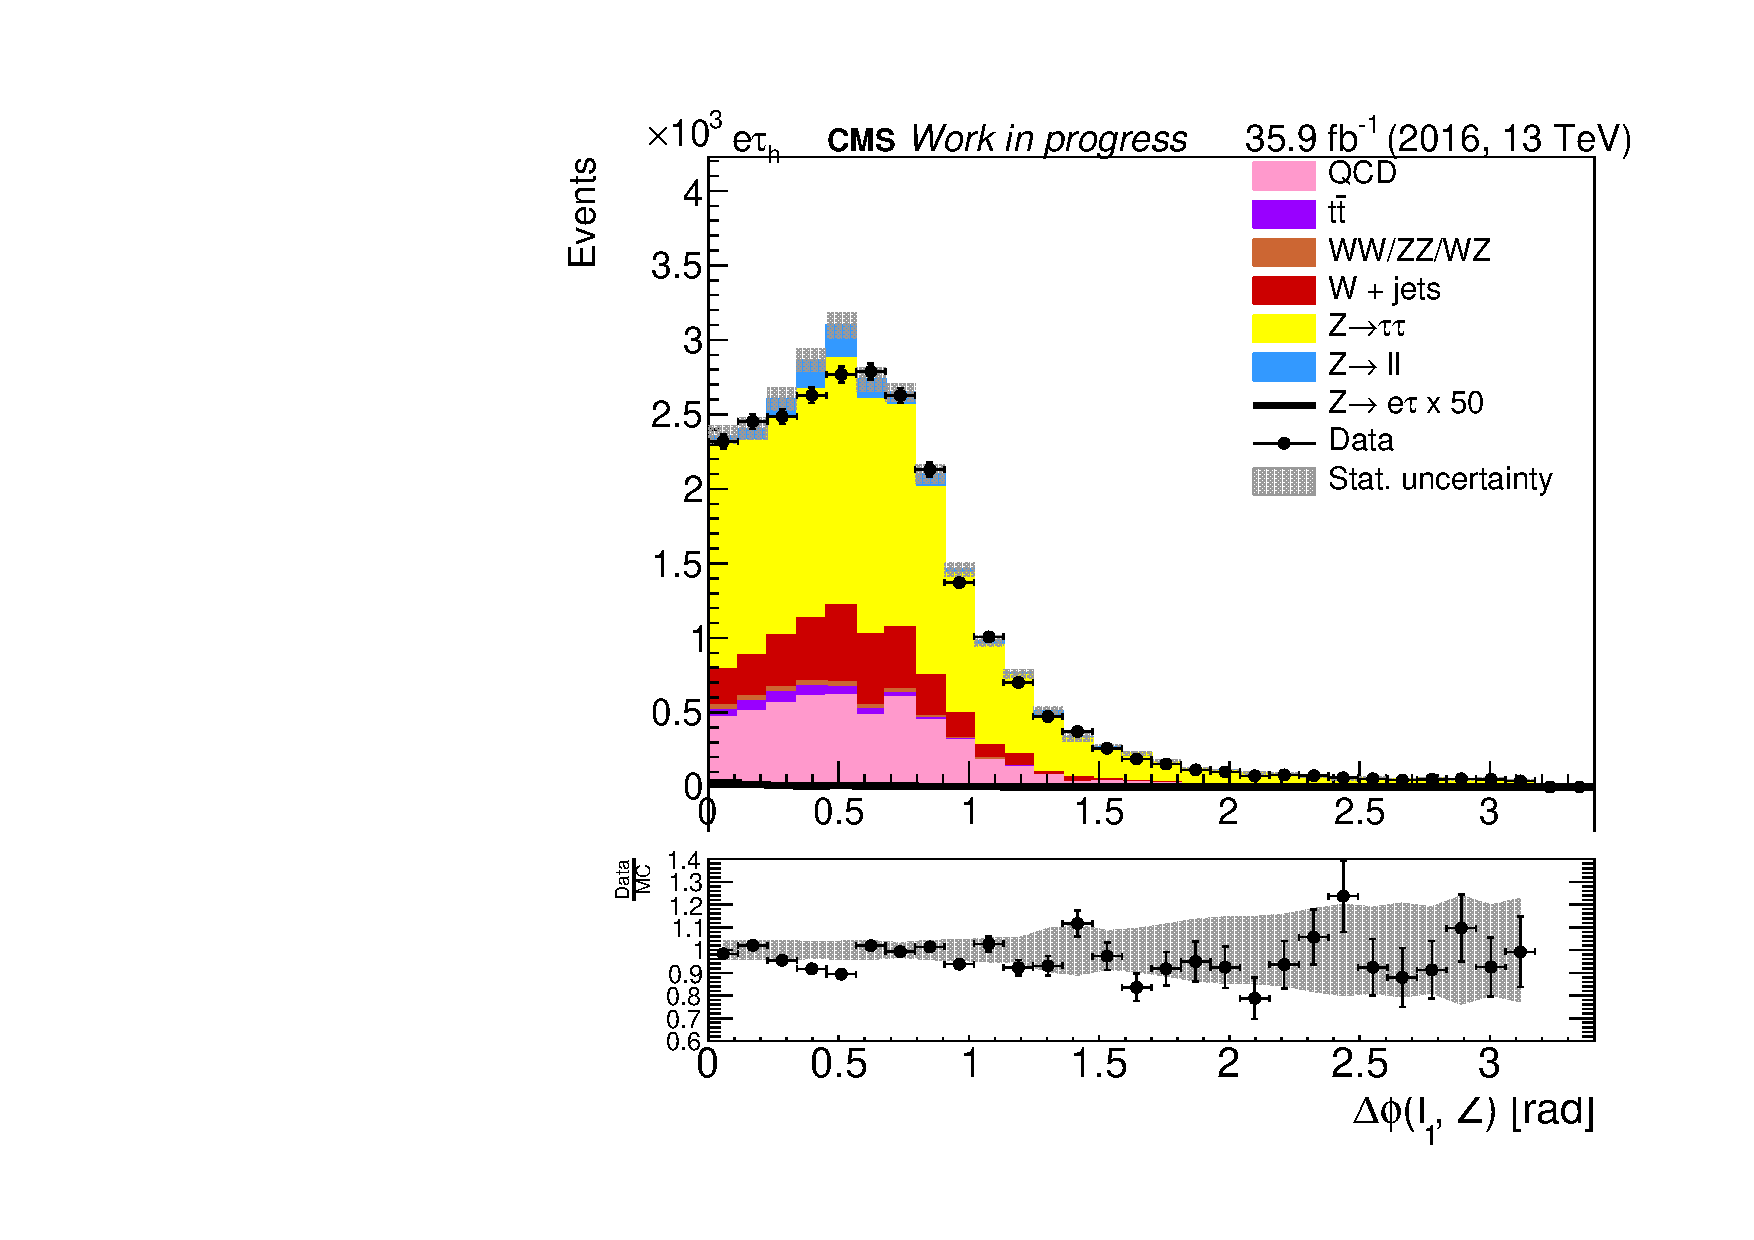
\includegraphics[width=0.45\textwidth]{plots/et/DeltaPhiL1Z_CR.pdf}
	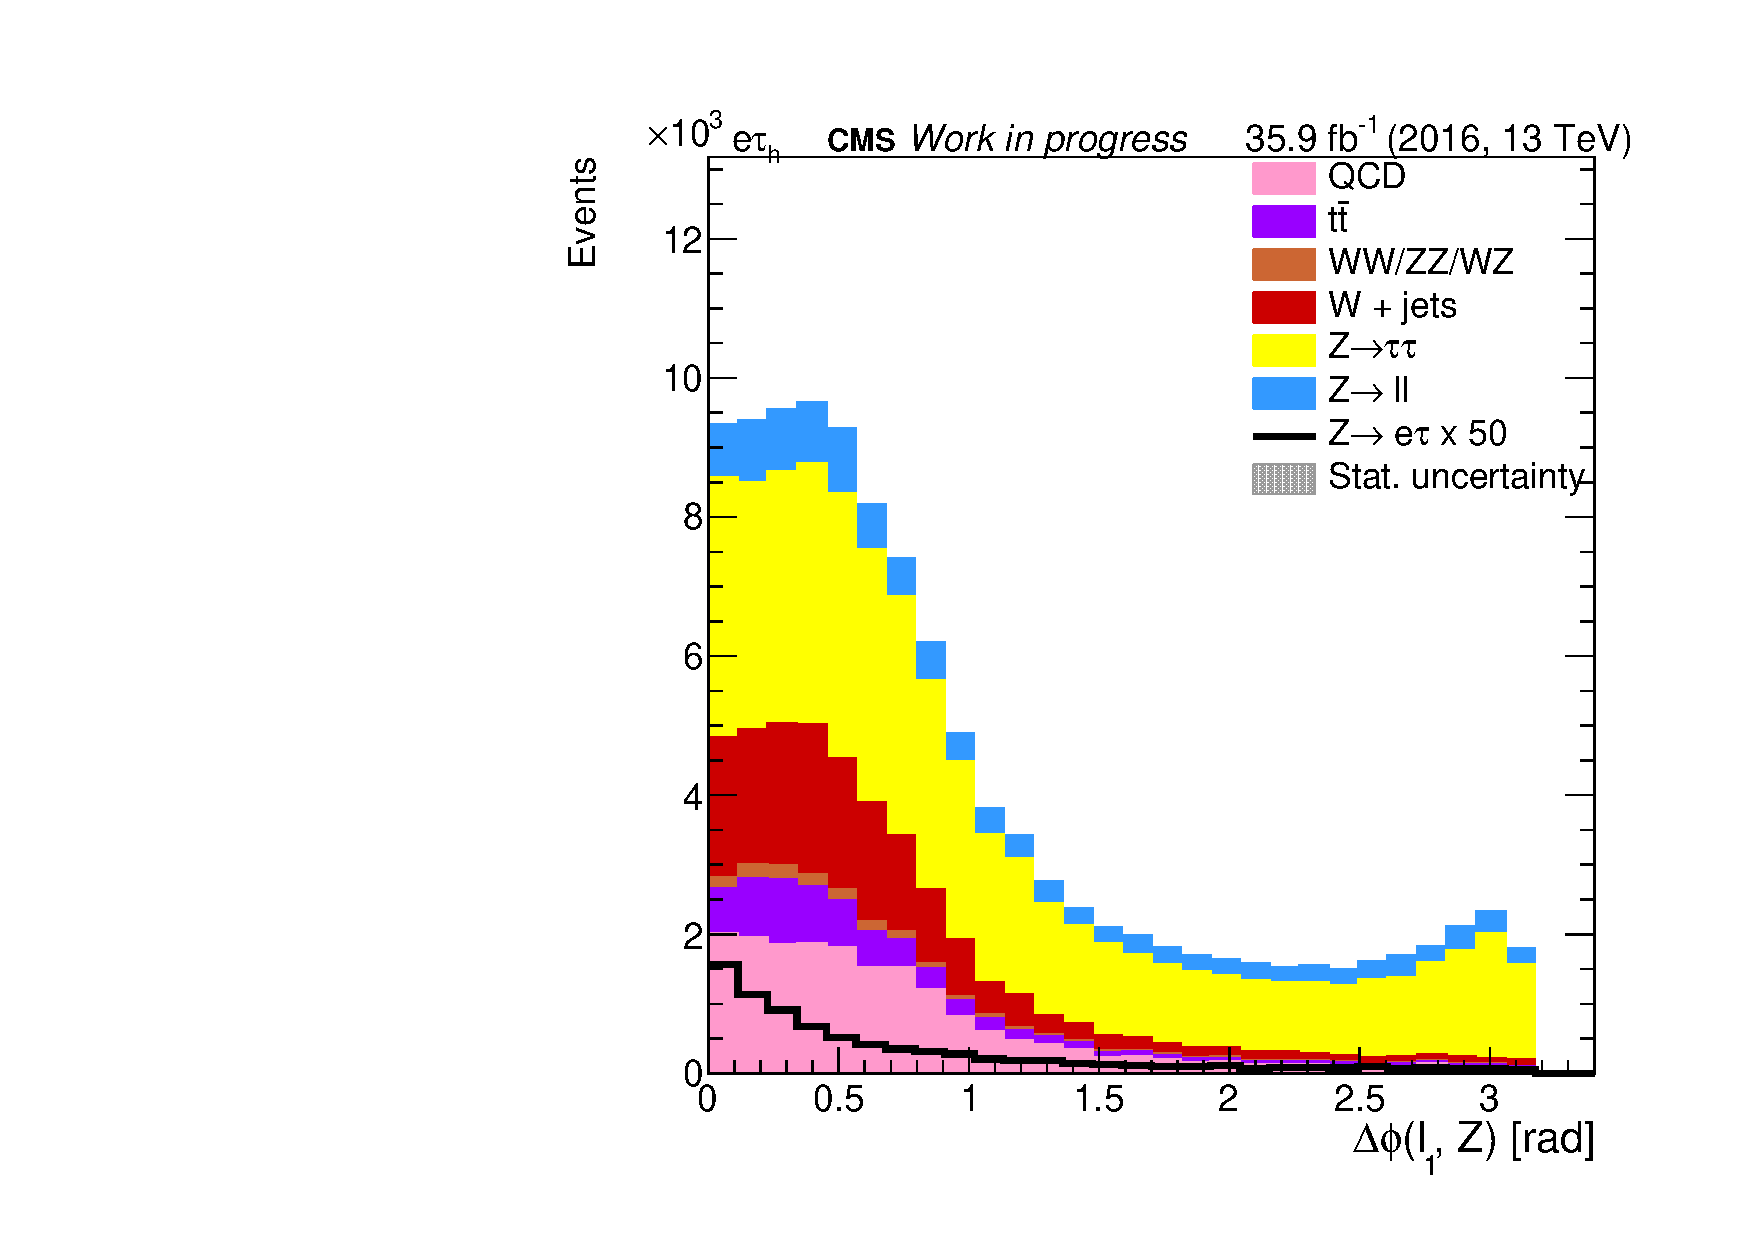
\includegraphics[width=0.45\textwidth]{plots/et/DeltaPhiL1Z_withsignal.pdf}

\end{figure}


\begin{figure}[htp]
	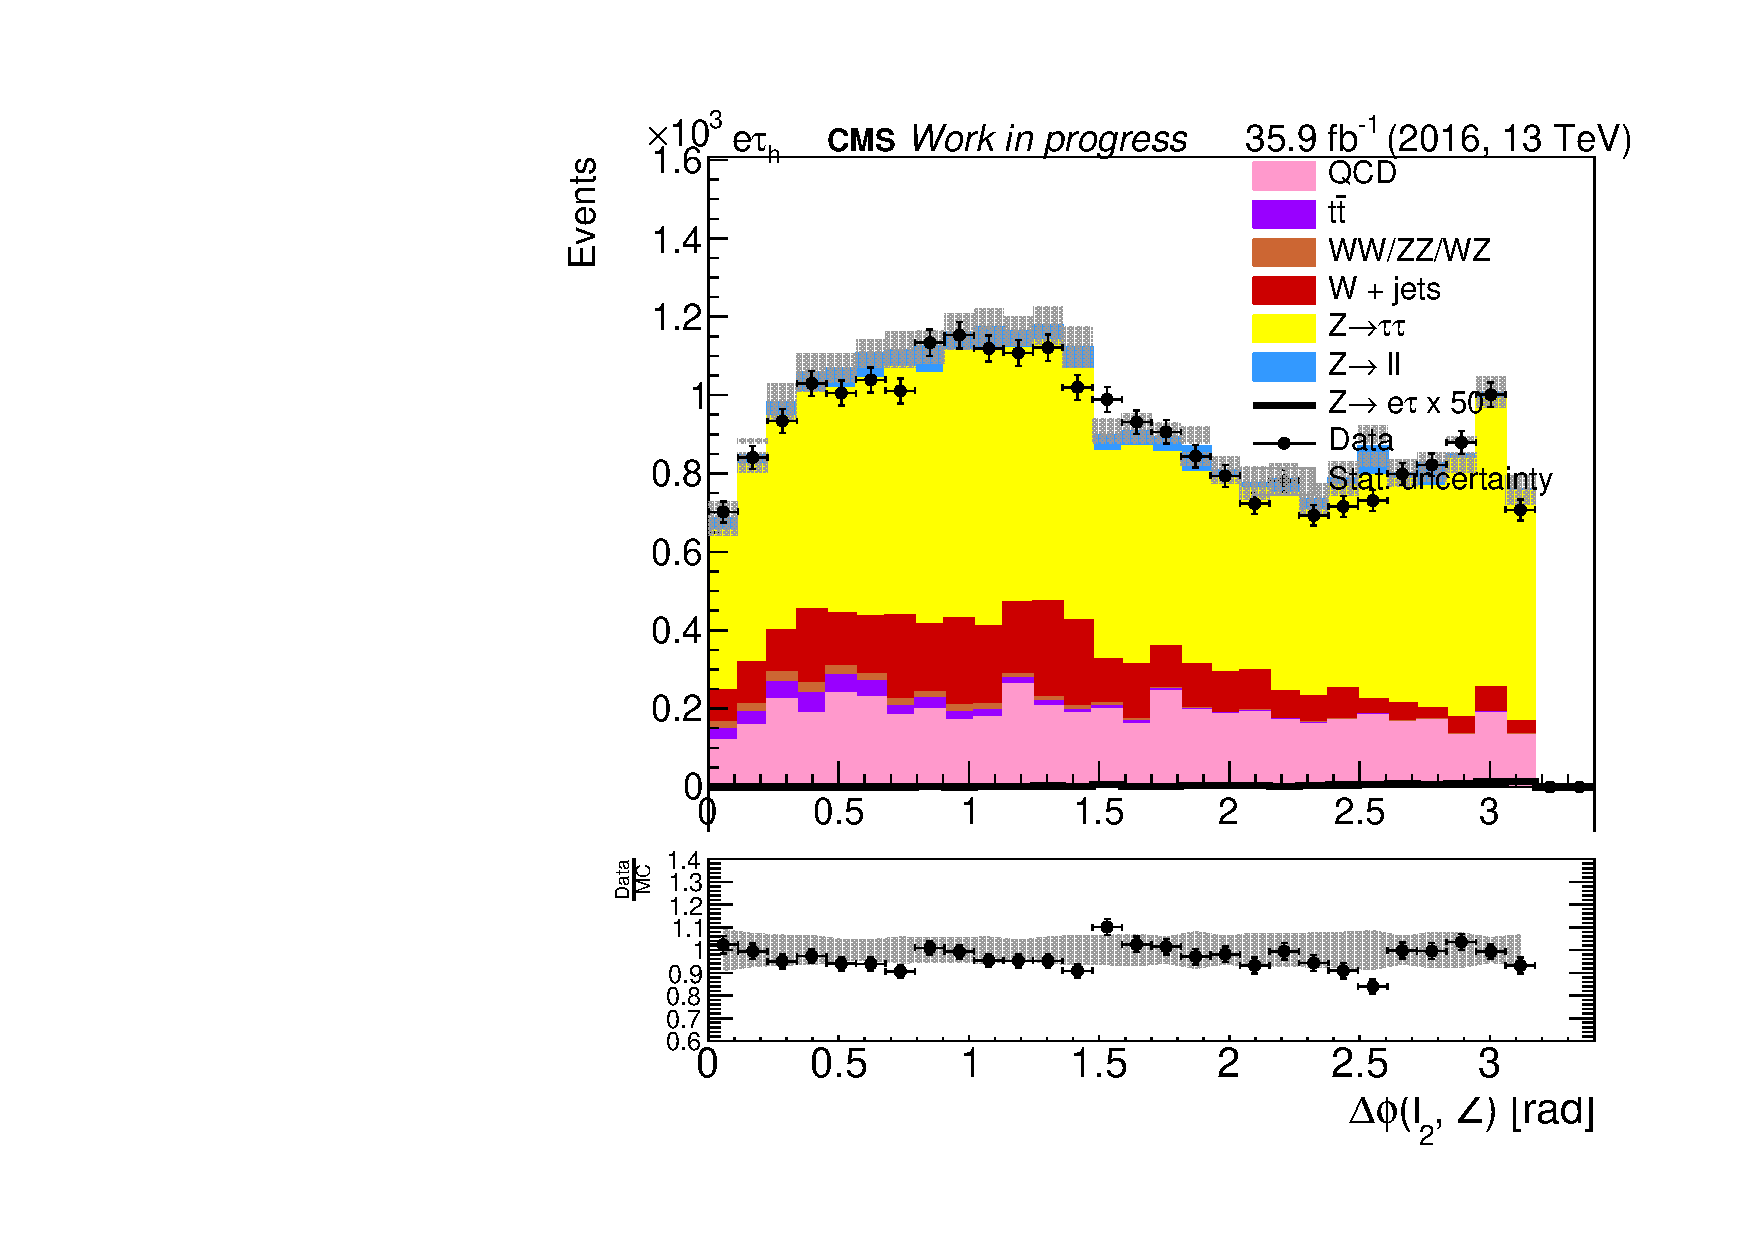
\includegraphics[width=0.45\textwidth]{plots/et/DeltaPhiL2Z_CR.pdf}
	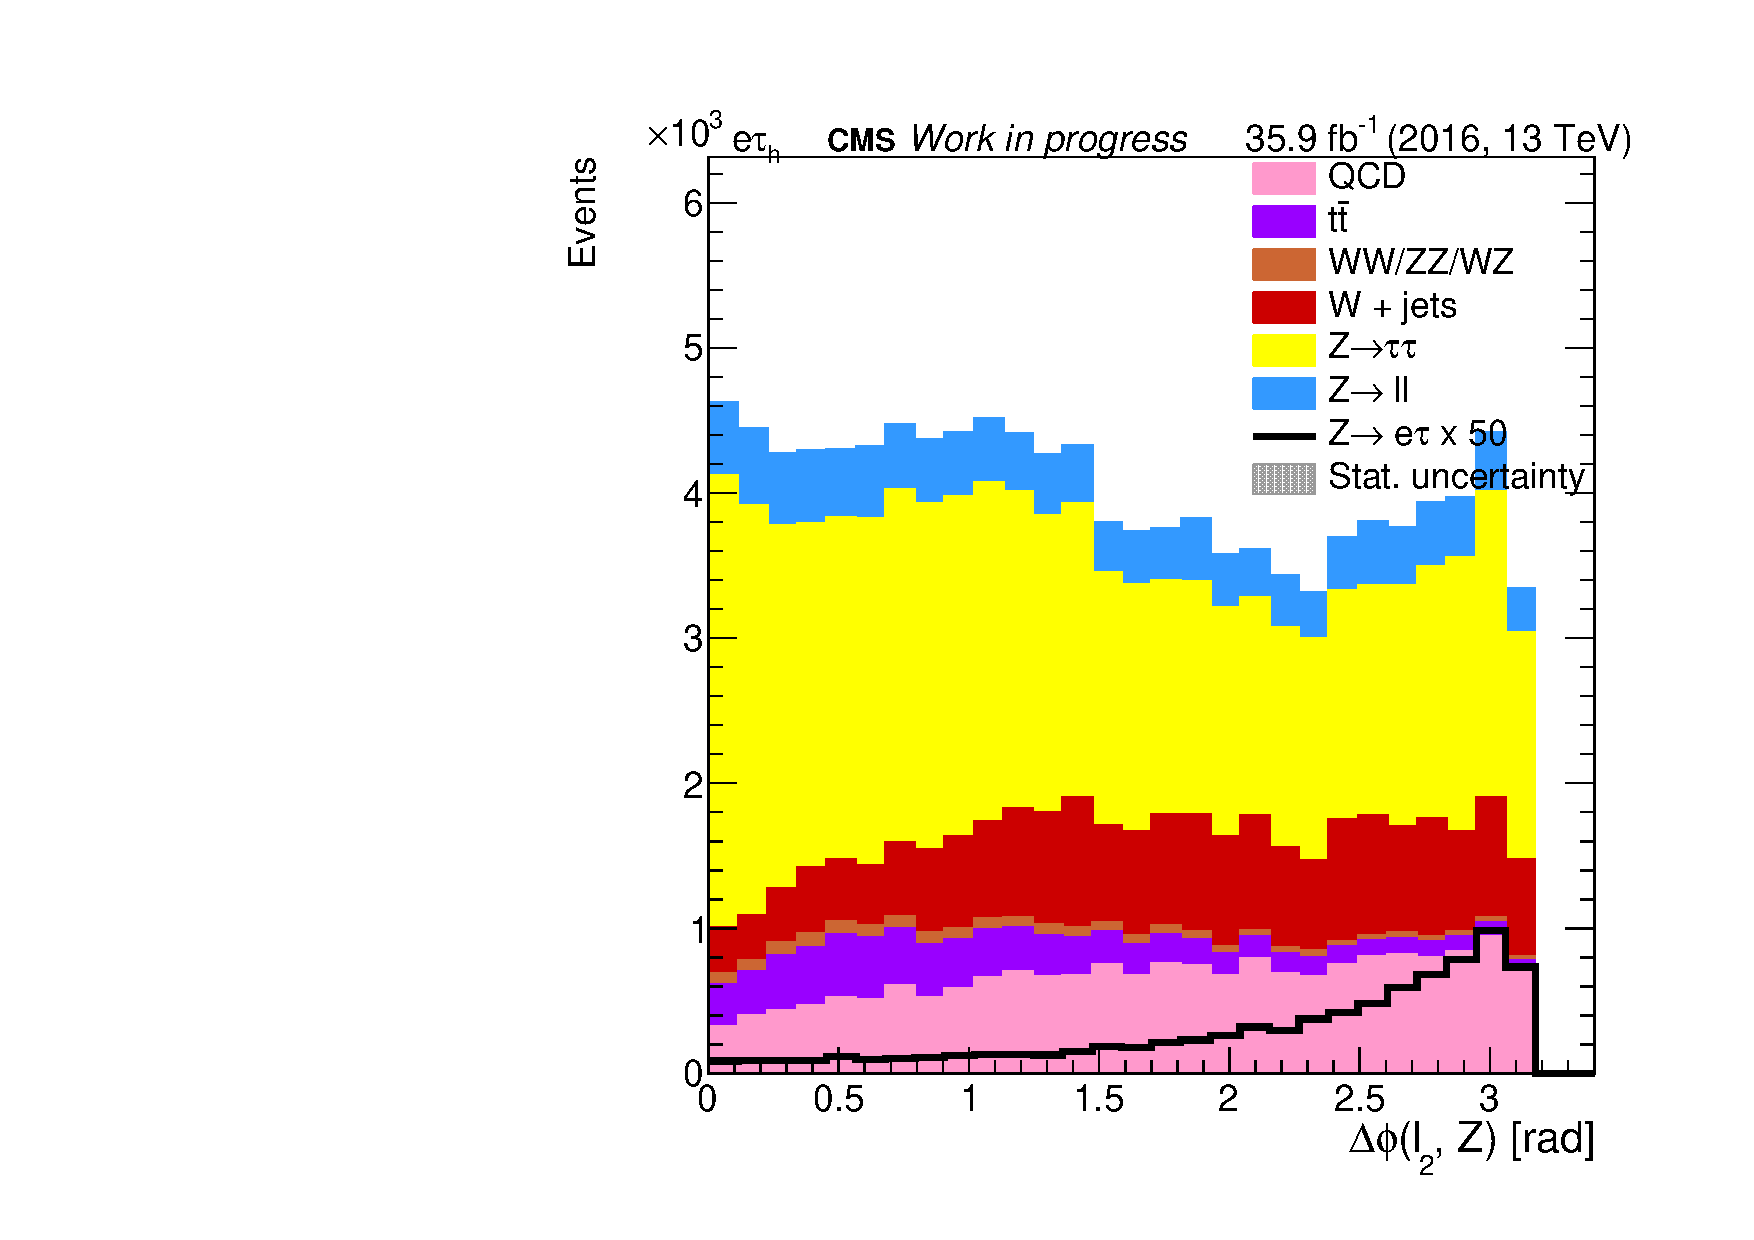
\includegraphics[width=0.45\textwidth]{plots/et/DeltaPhiL2Z_withsignal.pdf}

	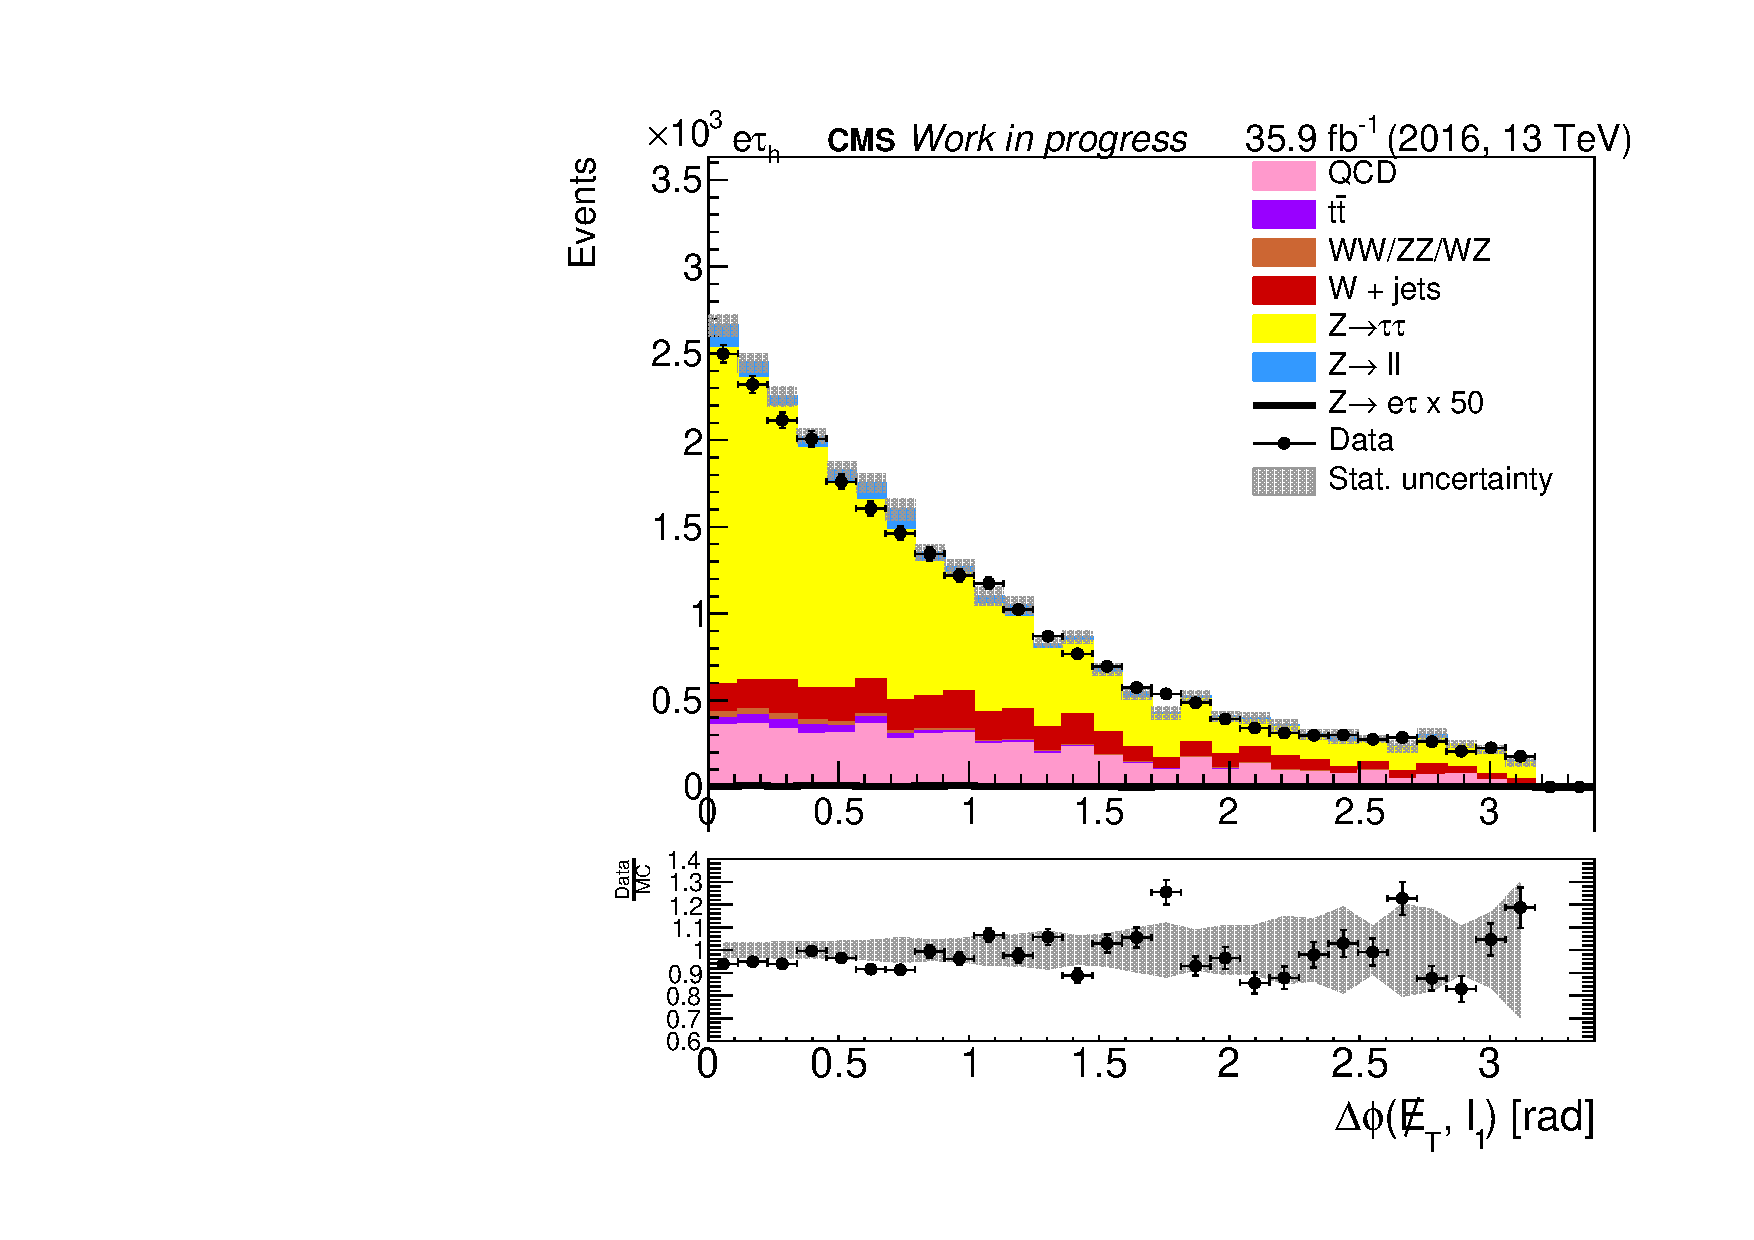
\includegraphics[width=0.45\textwidth]{plots/et/DeltaPhiMetL1_CR.pdf}
	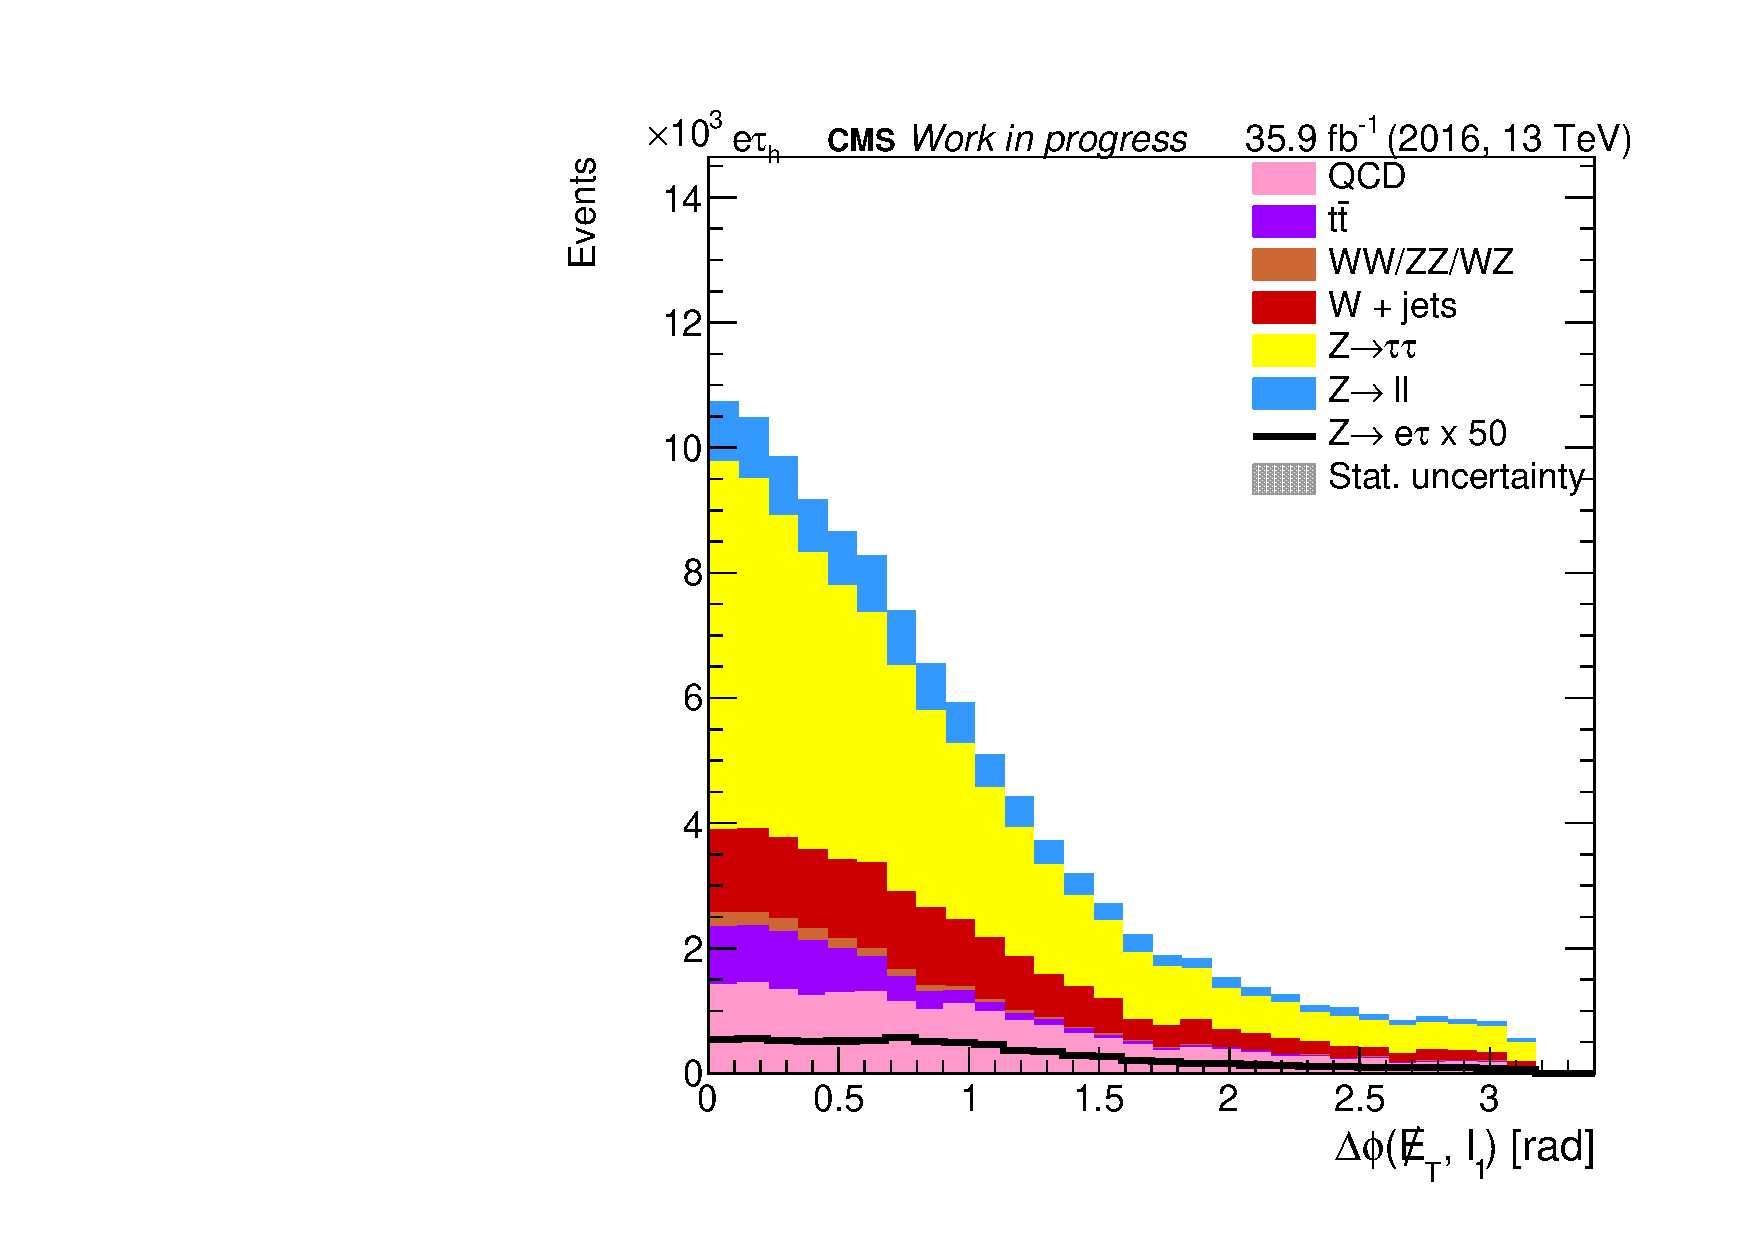
\includegraphics[width=0.45\textwidth]{plots/et/DeltaPhiMetL1_withsignal.pdf}

	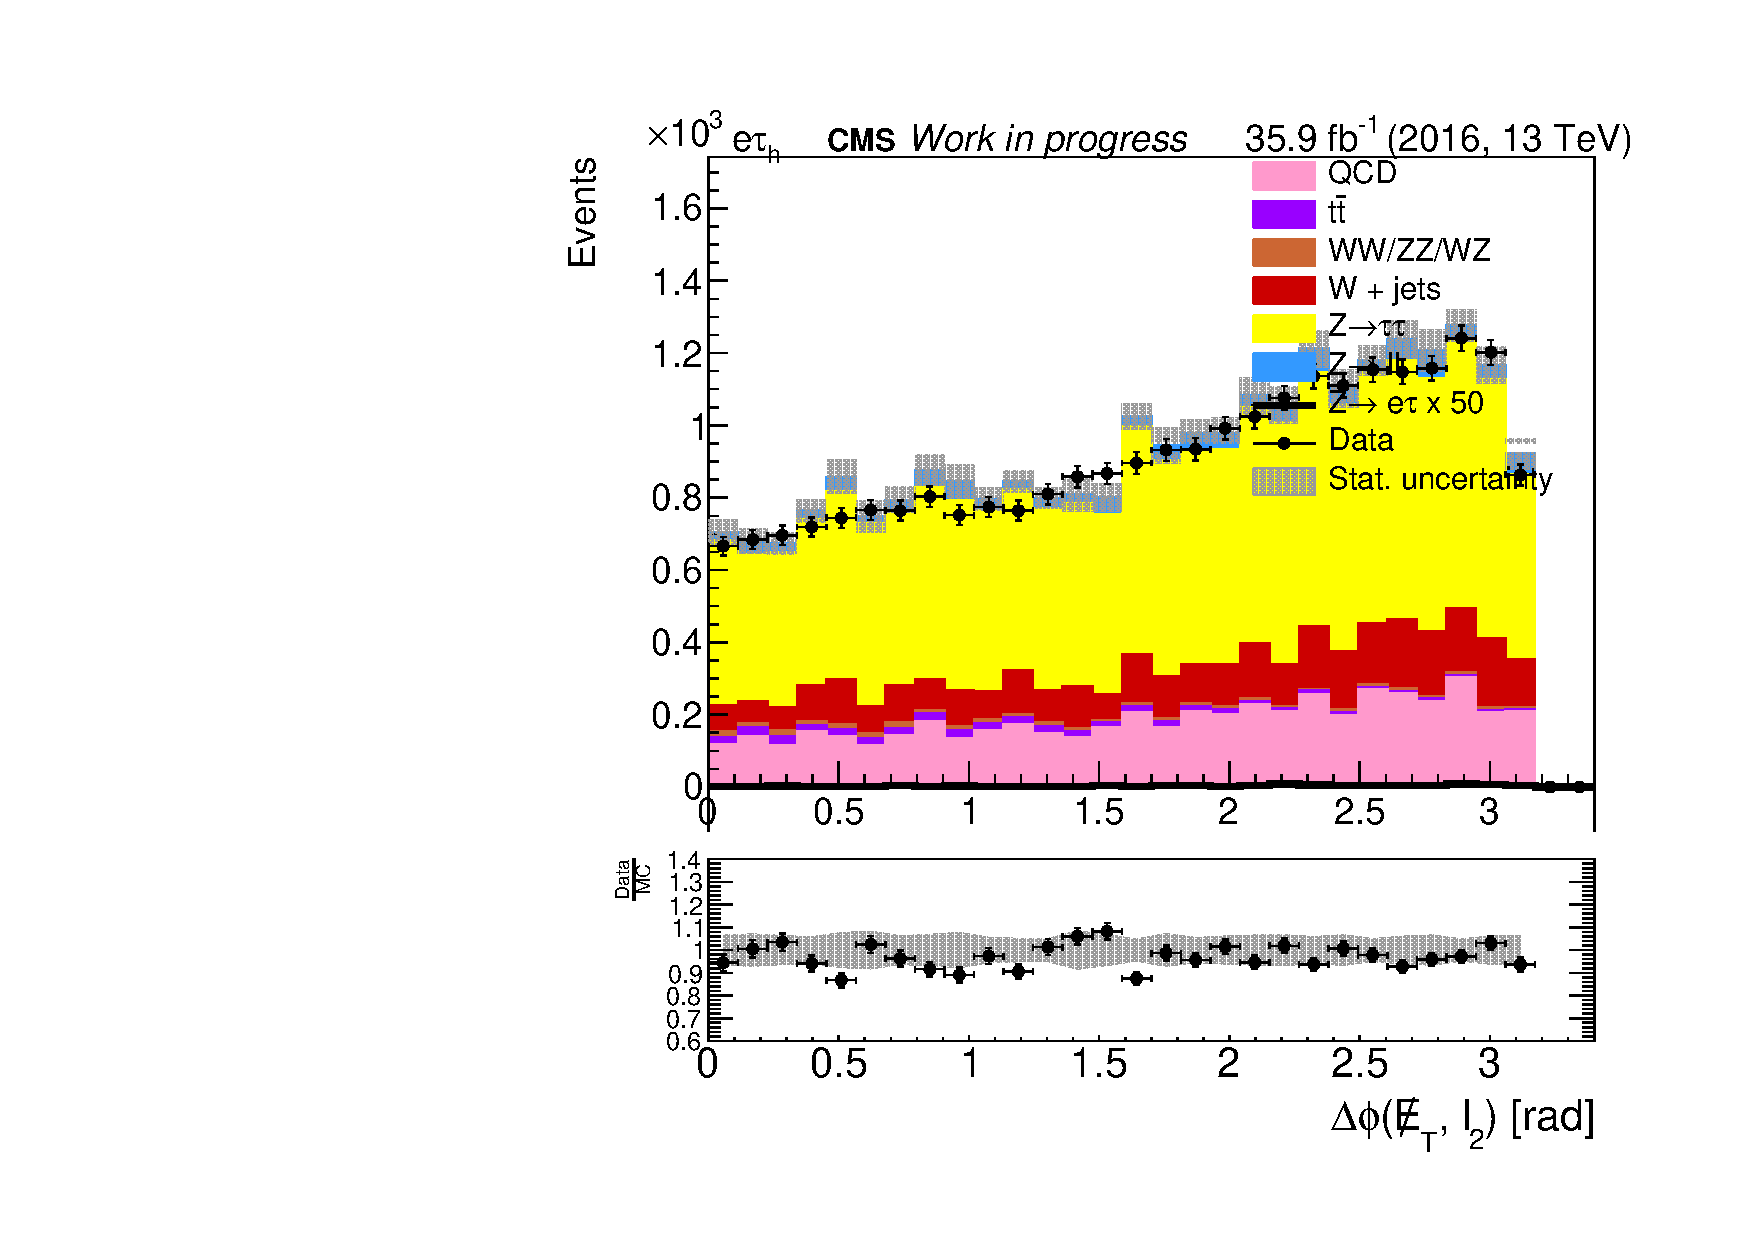
\includegraphics[width=0.45\textwidth]{plots/et/DeltaPhiMetL2_CR.pdf}
	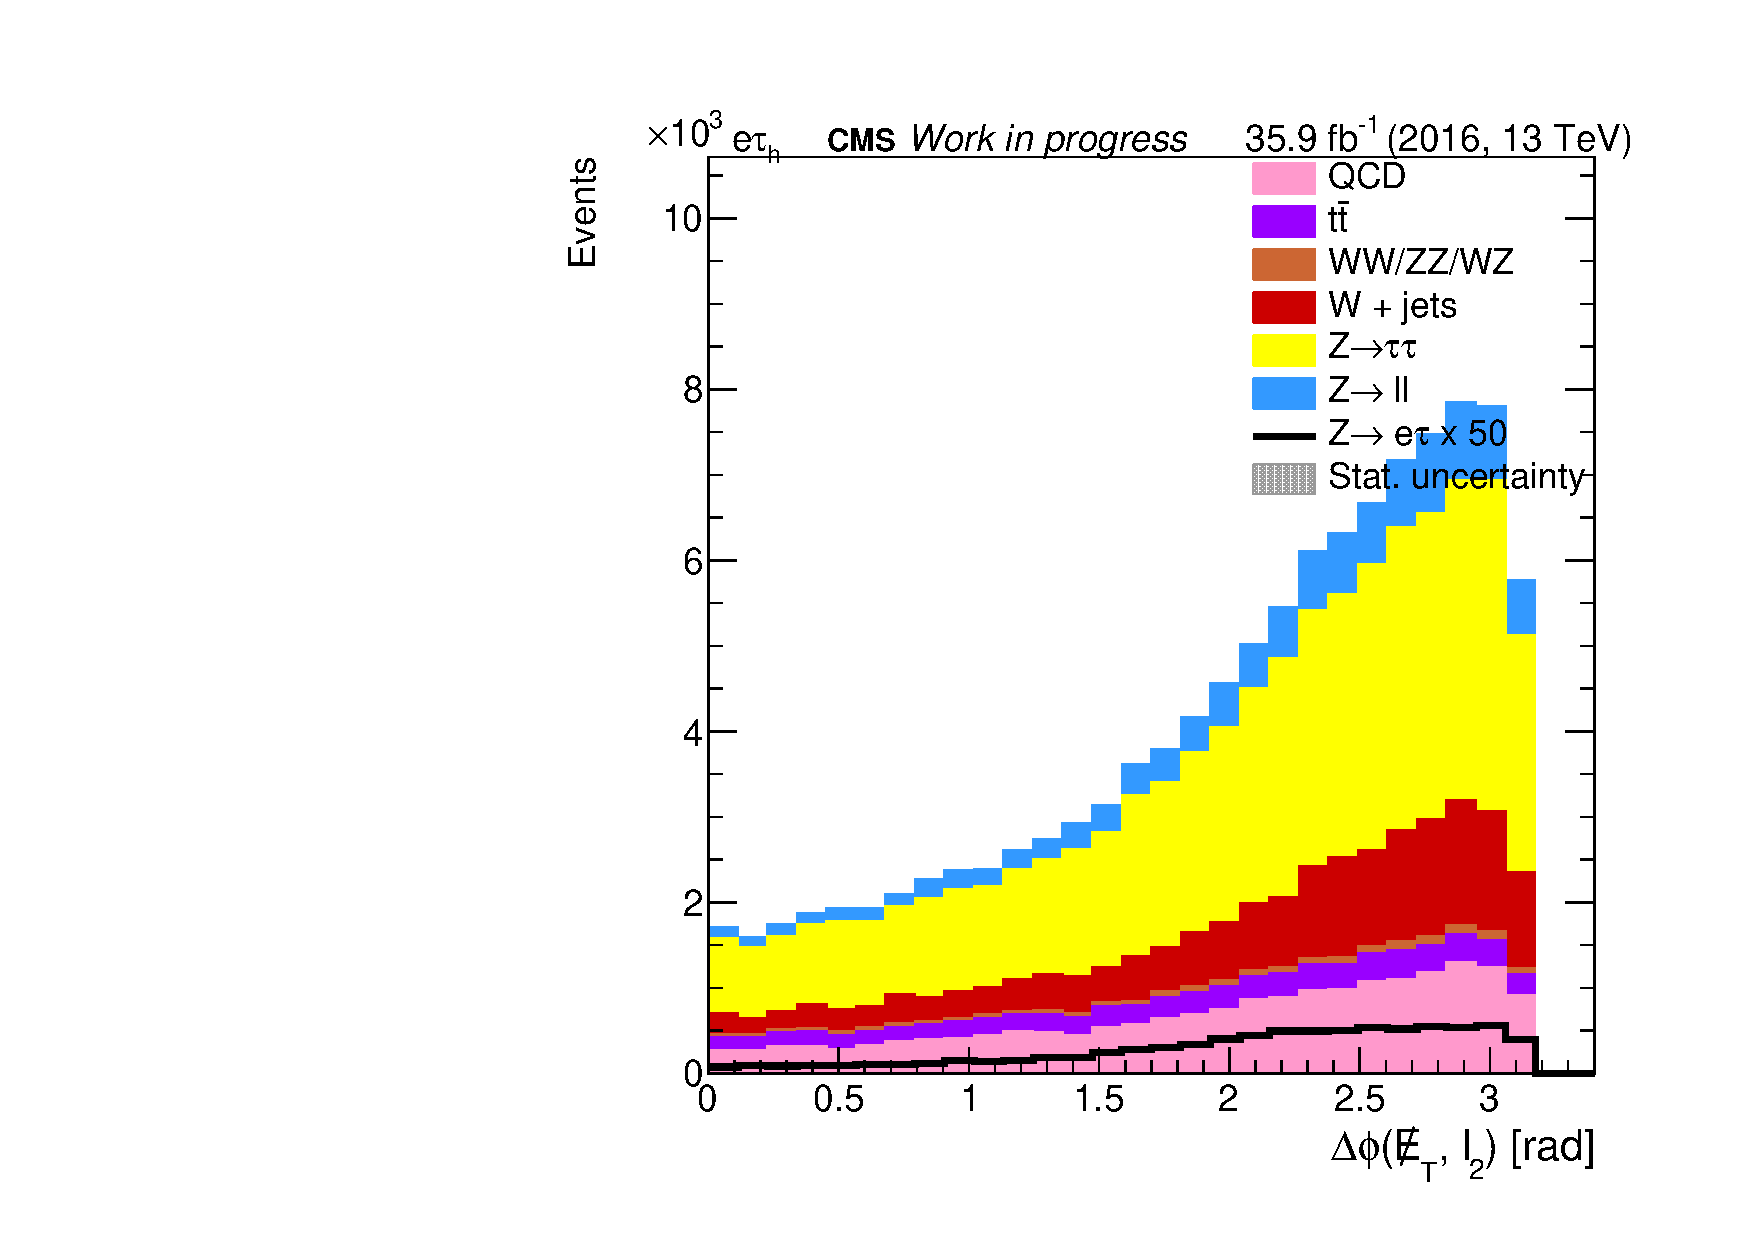
\includegraphics[width=0.45\textwidth]{plots/et/DeltaPhiMetL2_withsignal.pdf}
\end{figure}


\begin{figure}[htp]
	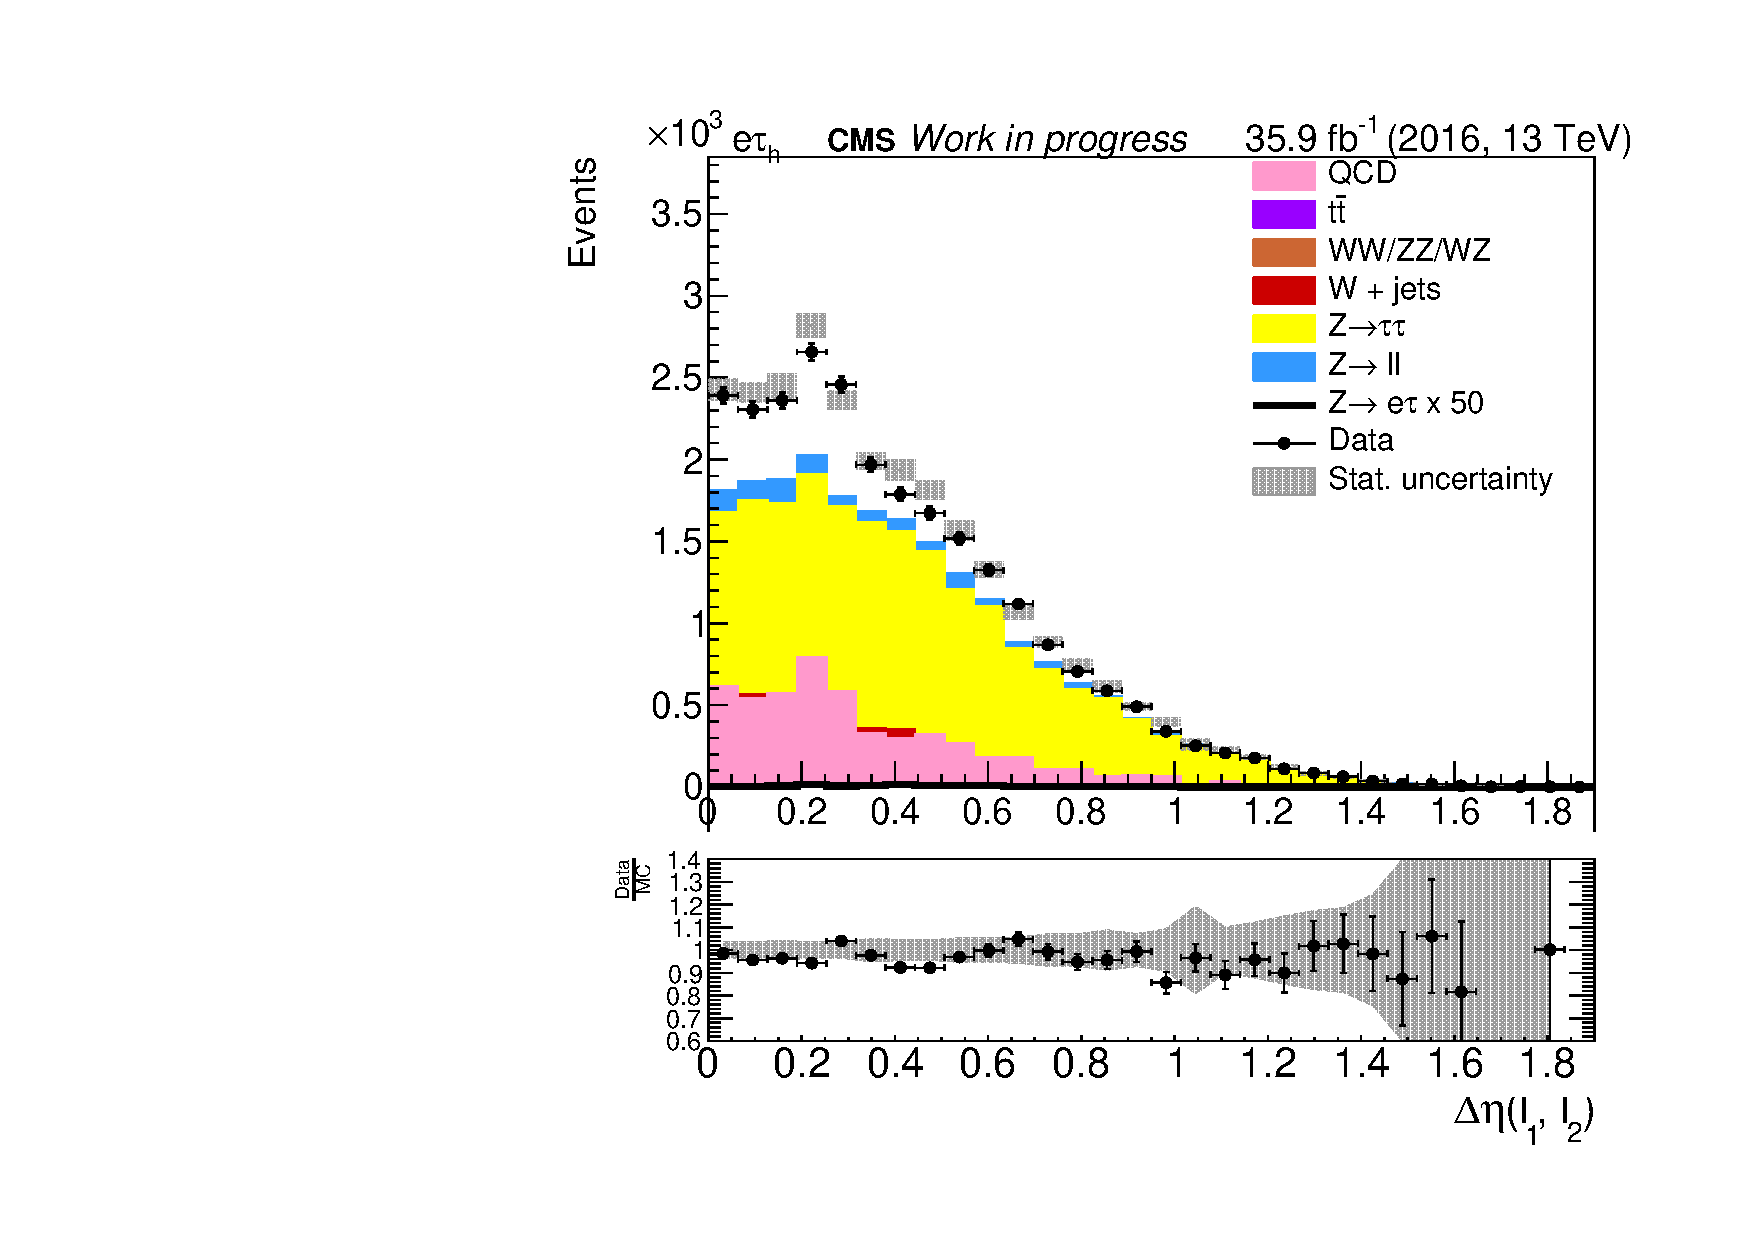
\includegraphics[width=0.45\textwidth]{plots/et/DiEta_CR.pdf}
	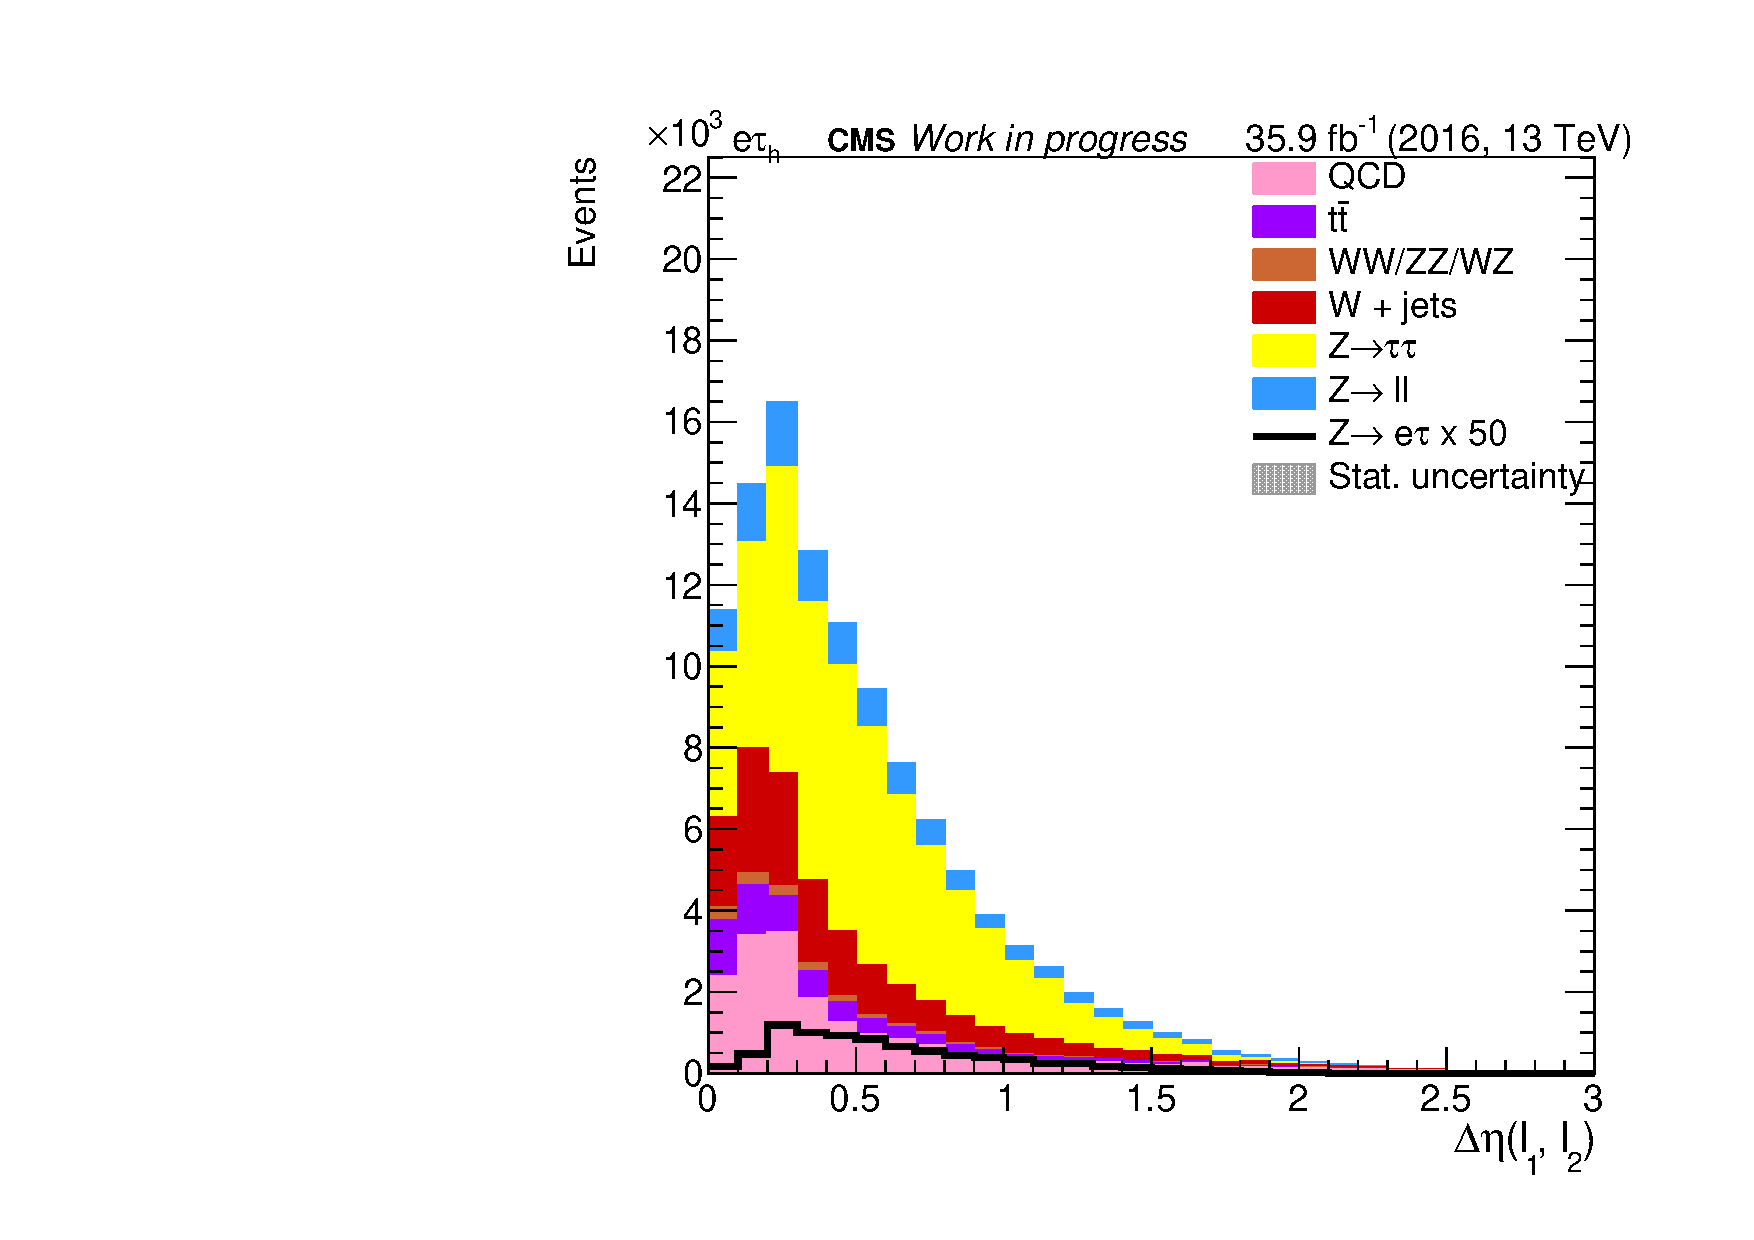
\includegraphics[width=0.45\textwidth]{plots/et/DiEta_withsignal.pdf}

	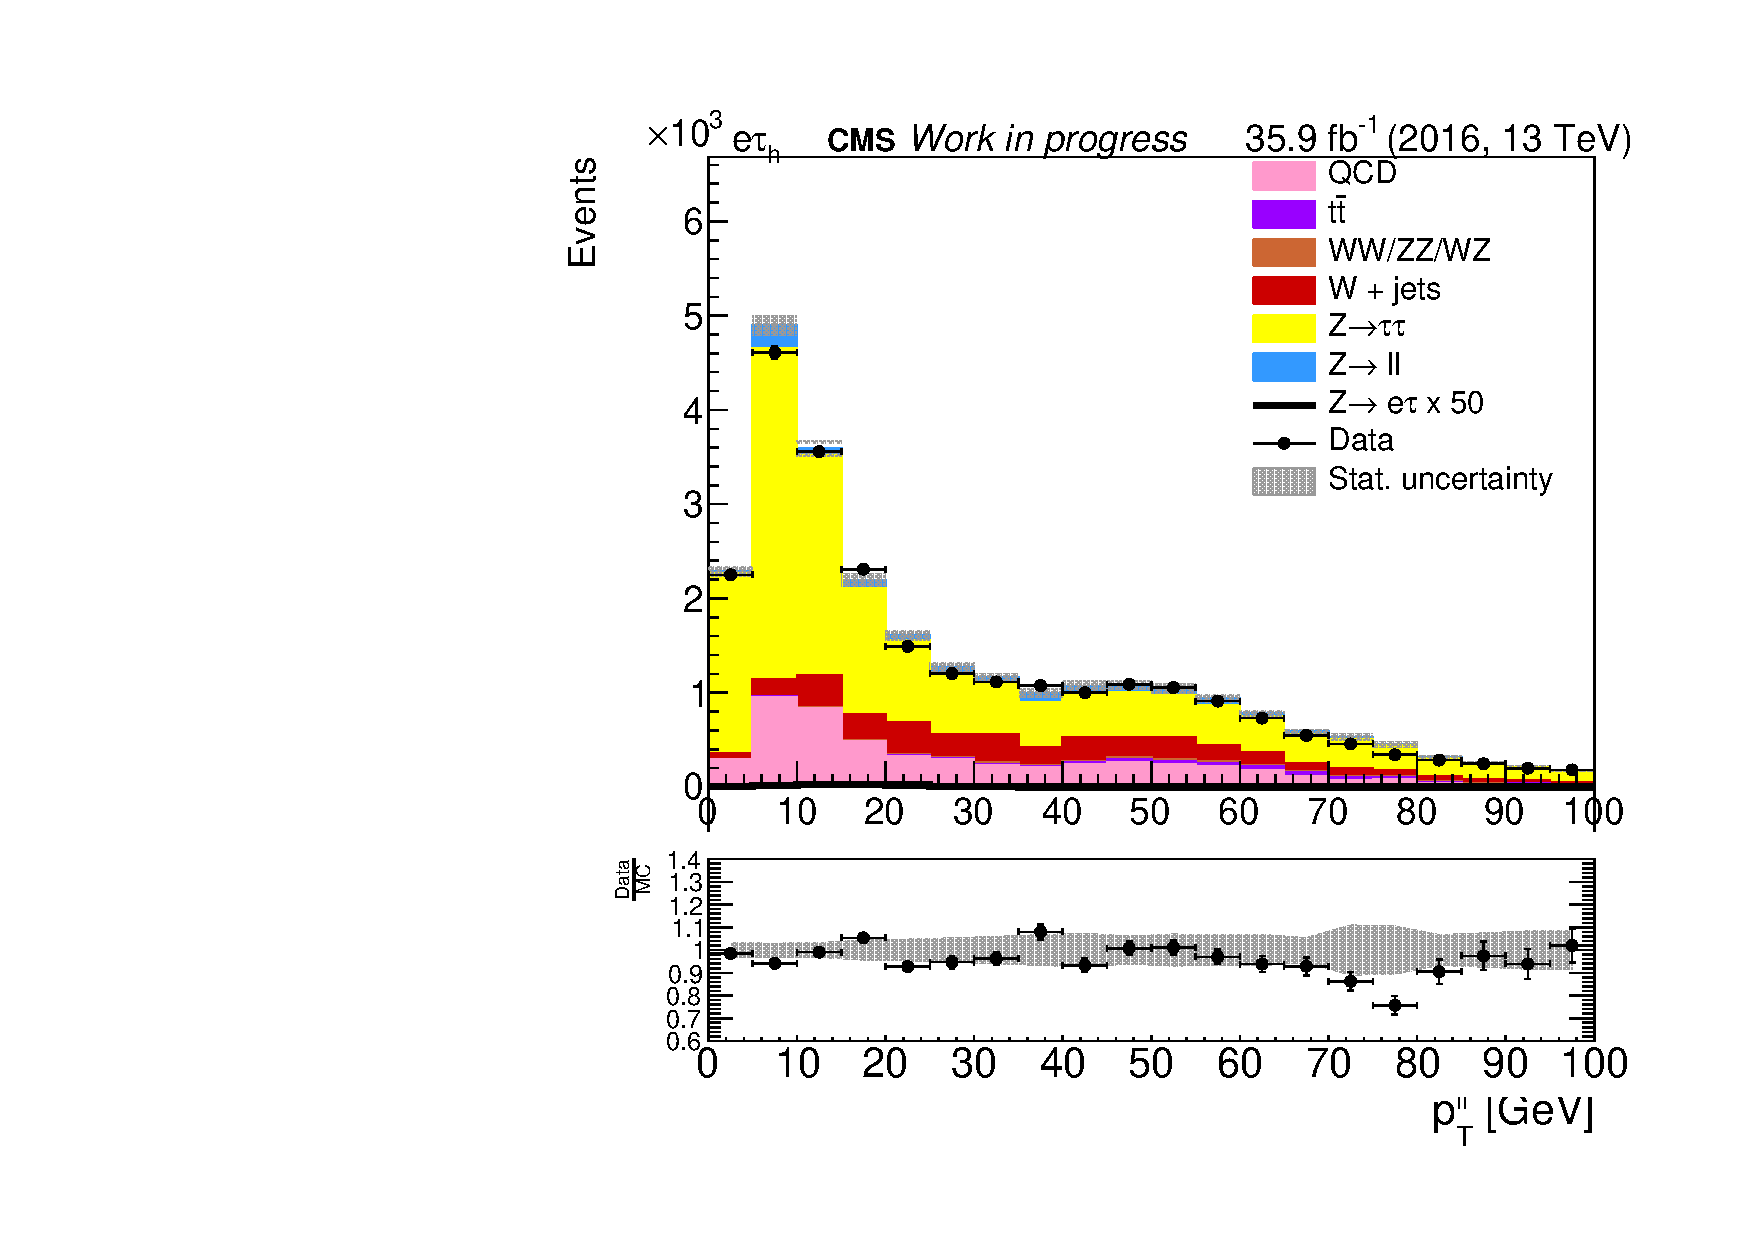
\includegraphics[width=0.45\textwidth]{plots/et/DiLepPt_CR.pdf}
	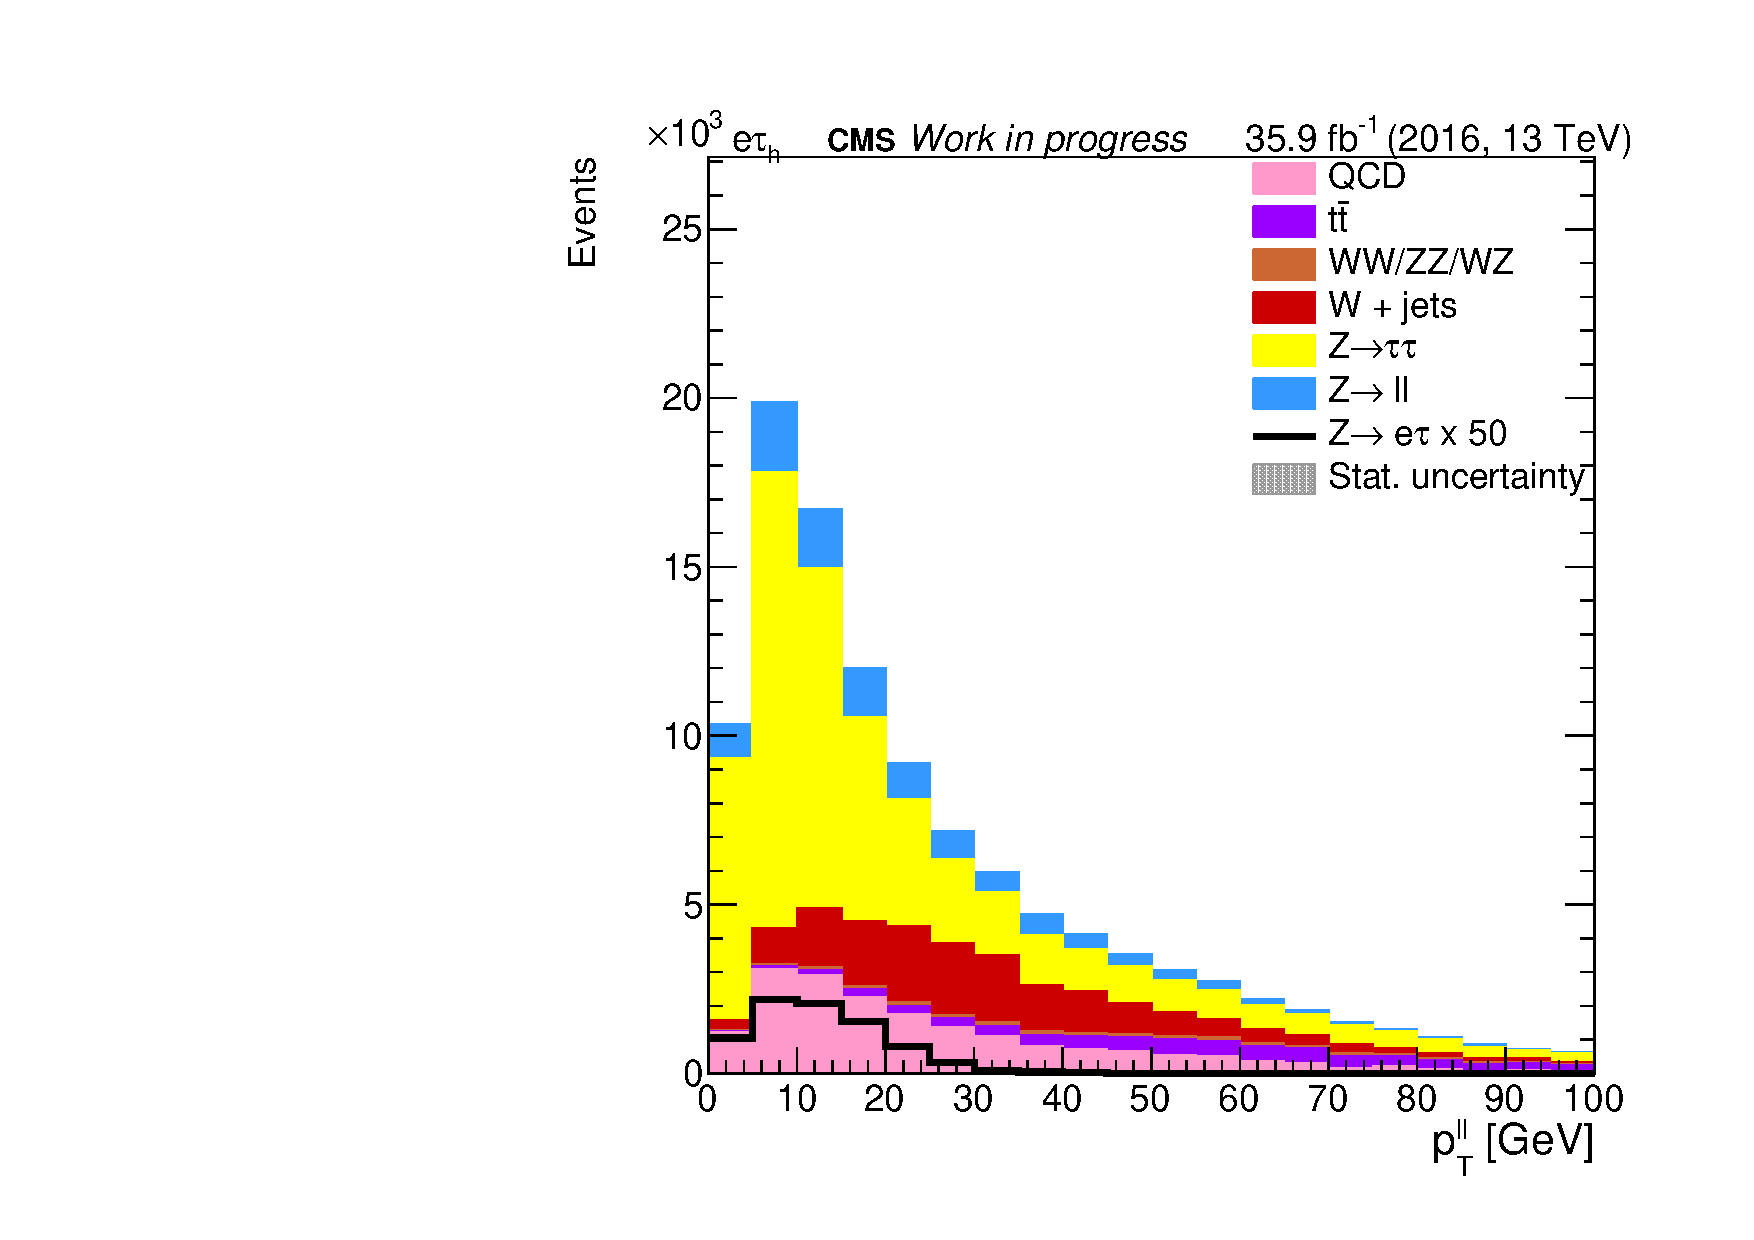
\includegraphics[width=0.45\textwidth]{plots/et/DiLepPt_withsignal.pdf}

	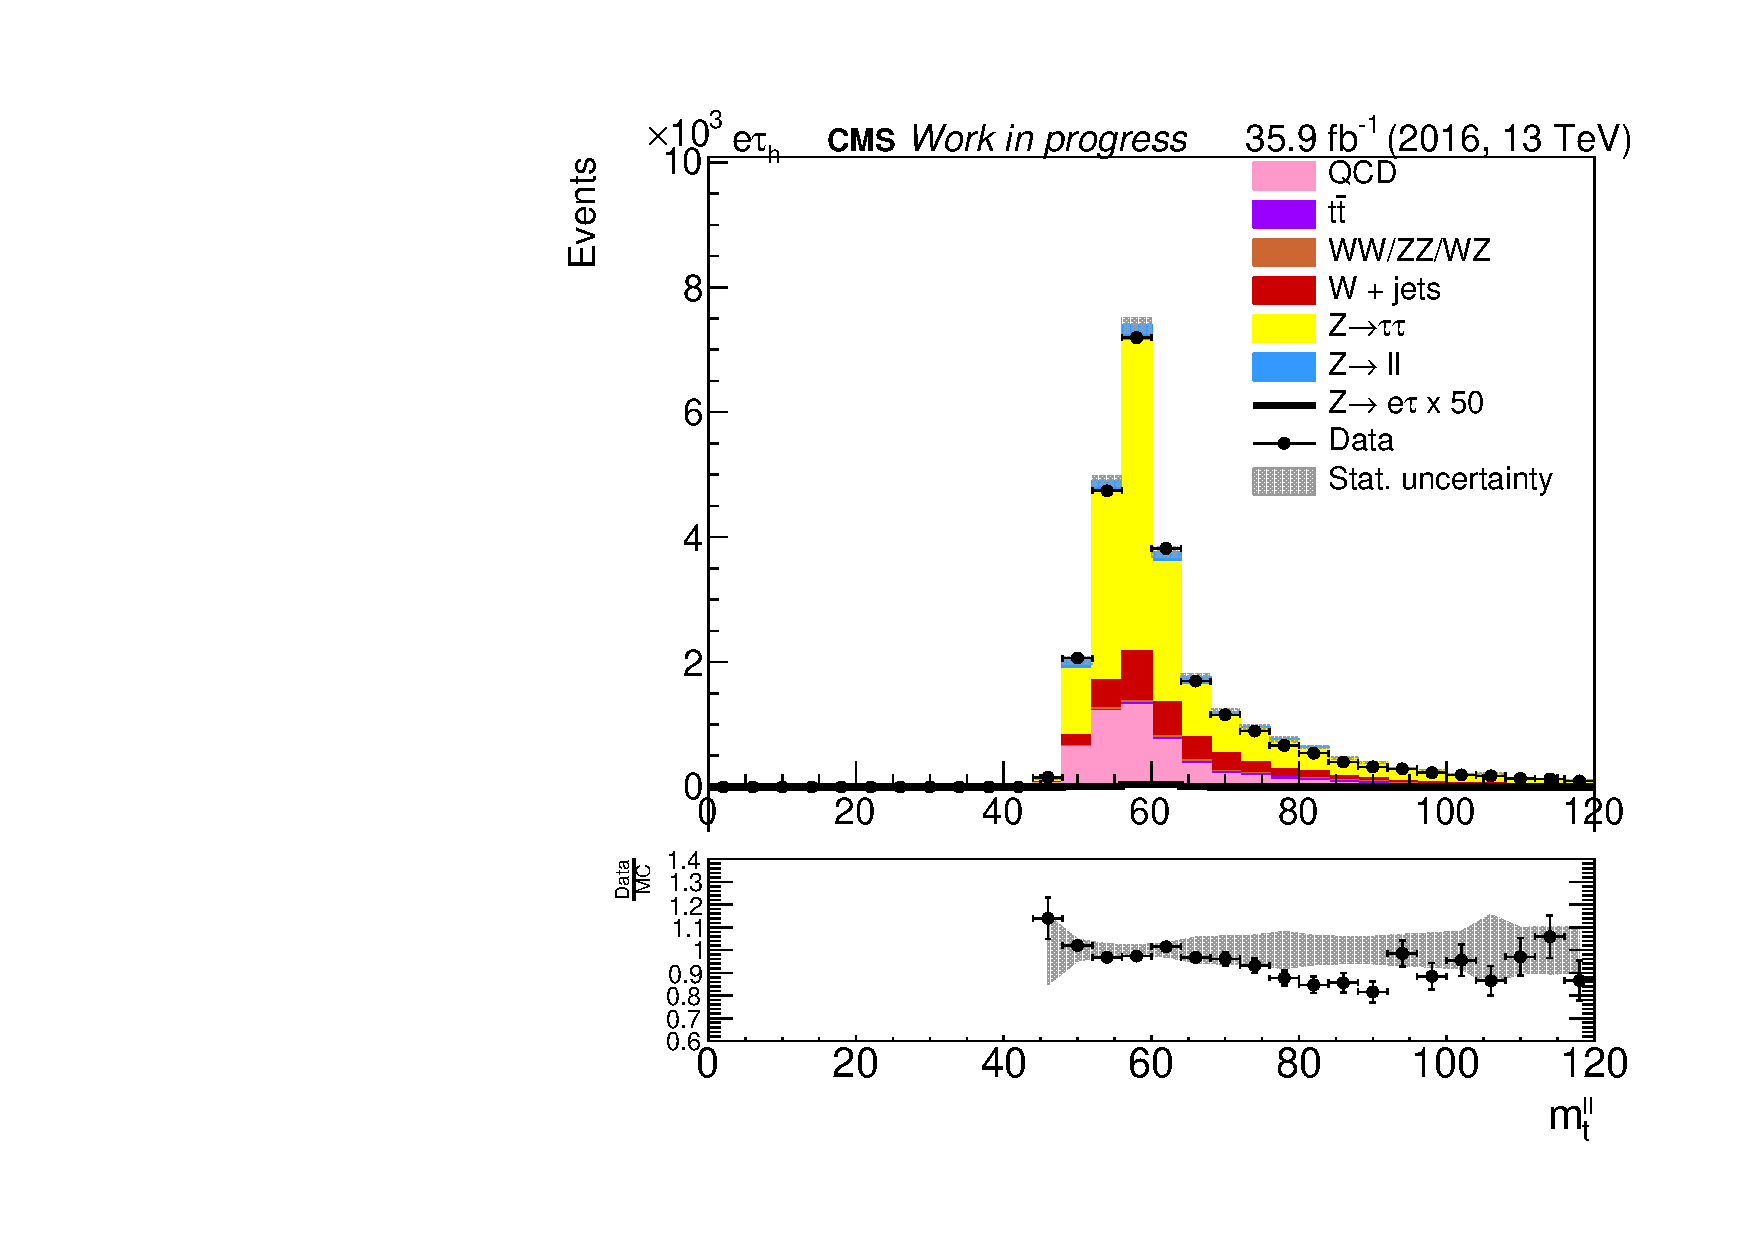
\includegraphics[width=0.45\textwidth]{plots/et/DiTransverseMass_CR.pdf}
	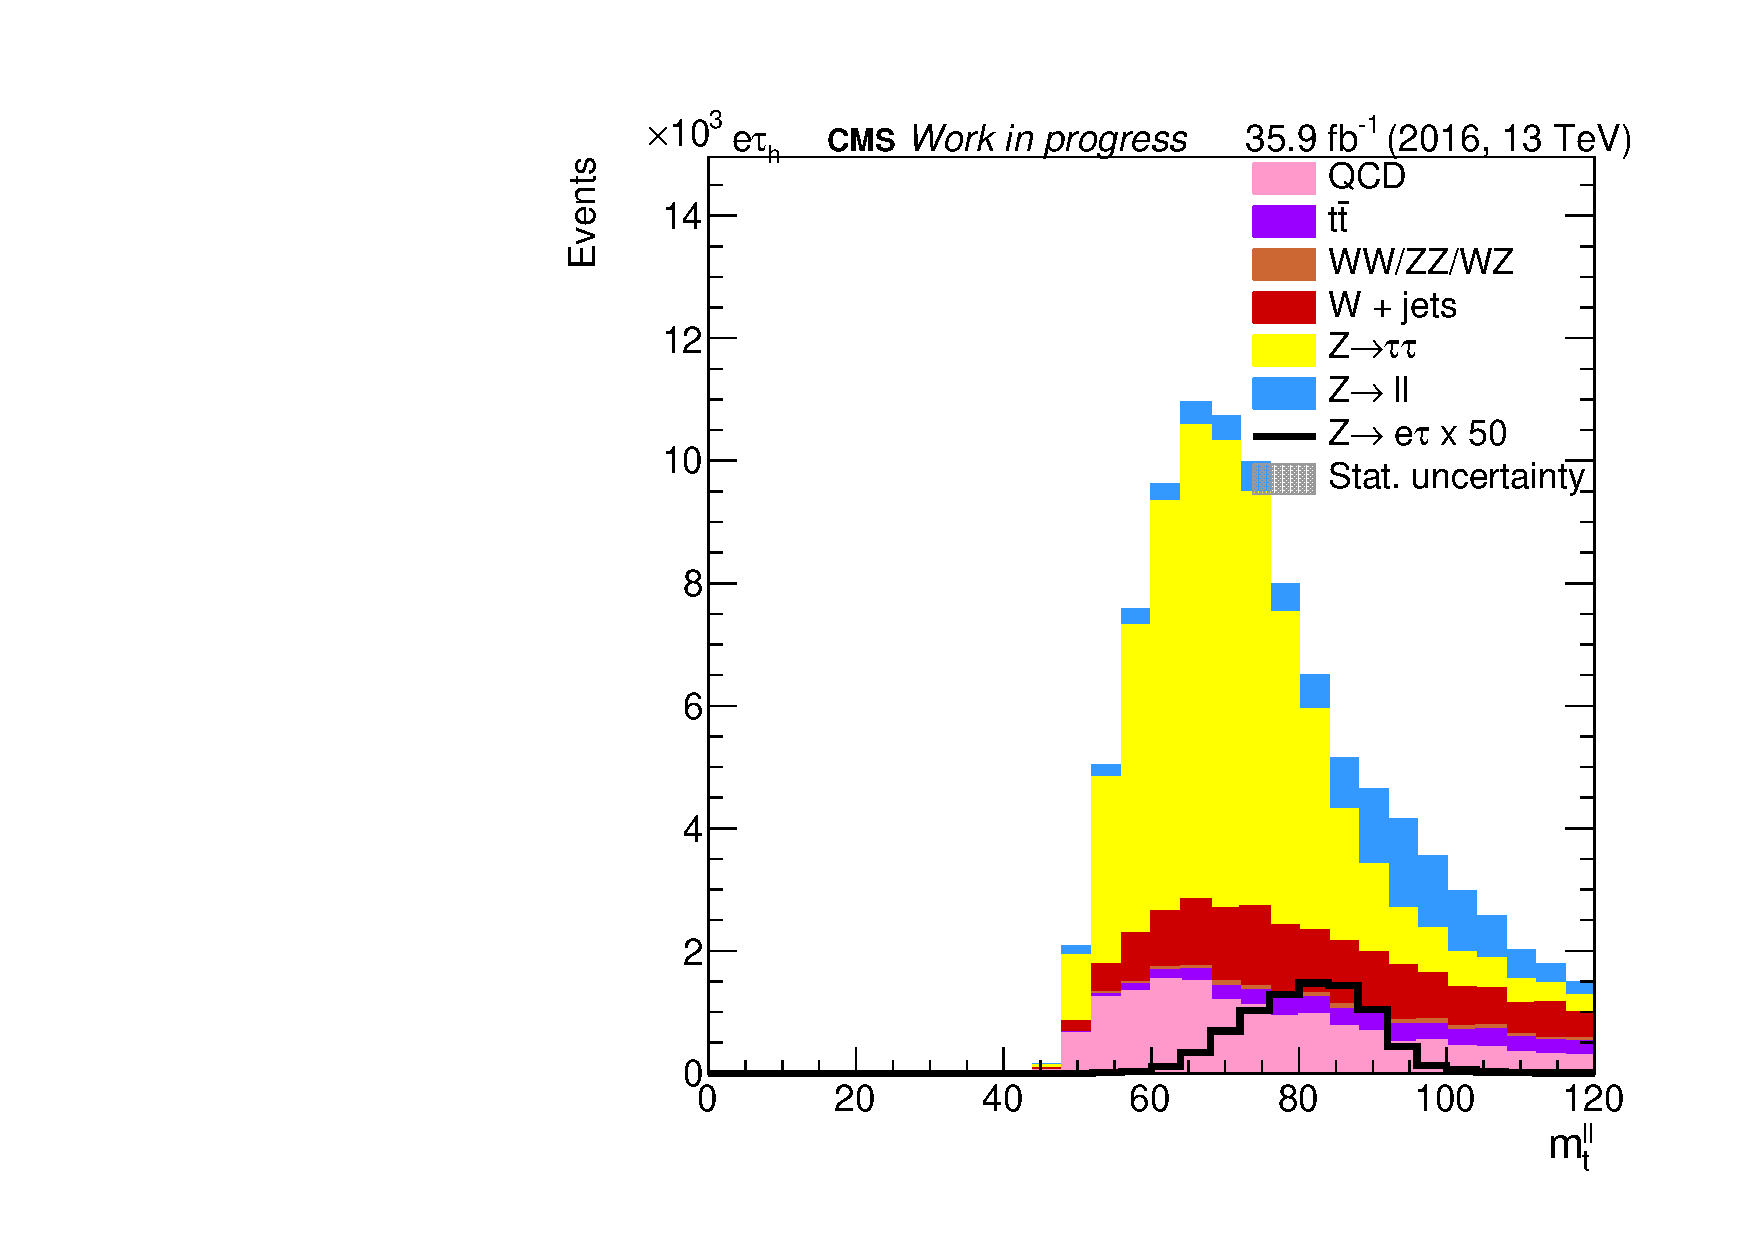
\includegraphics[width=0.45\textwidth]{plots/et/DiTransverseMass_withsignal.pdf}
\end{figure}


\begin{figure}[htp]
	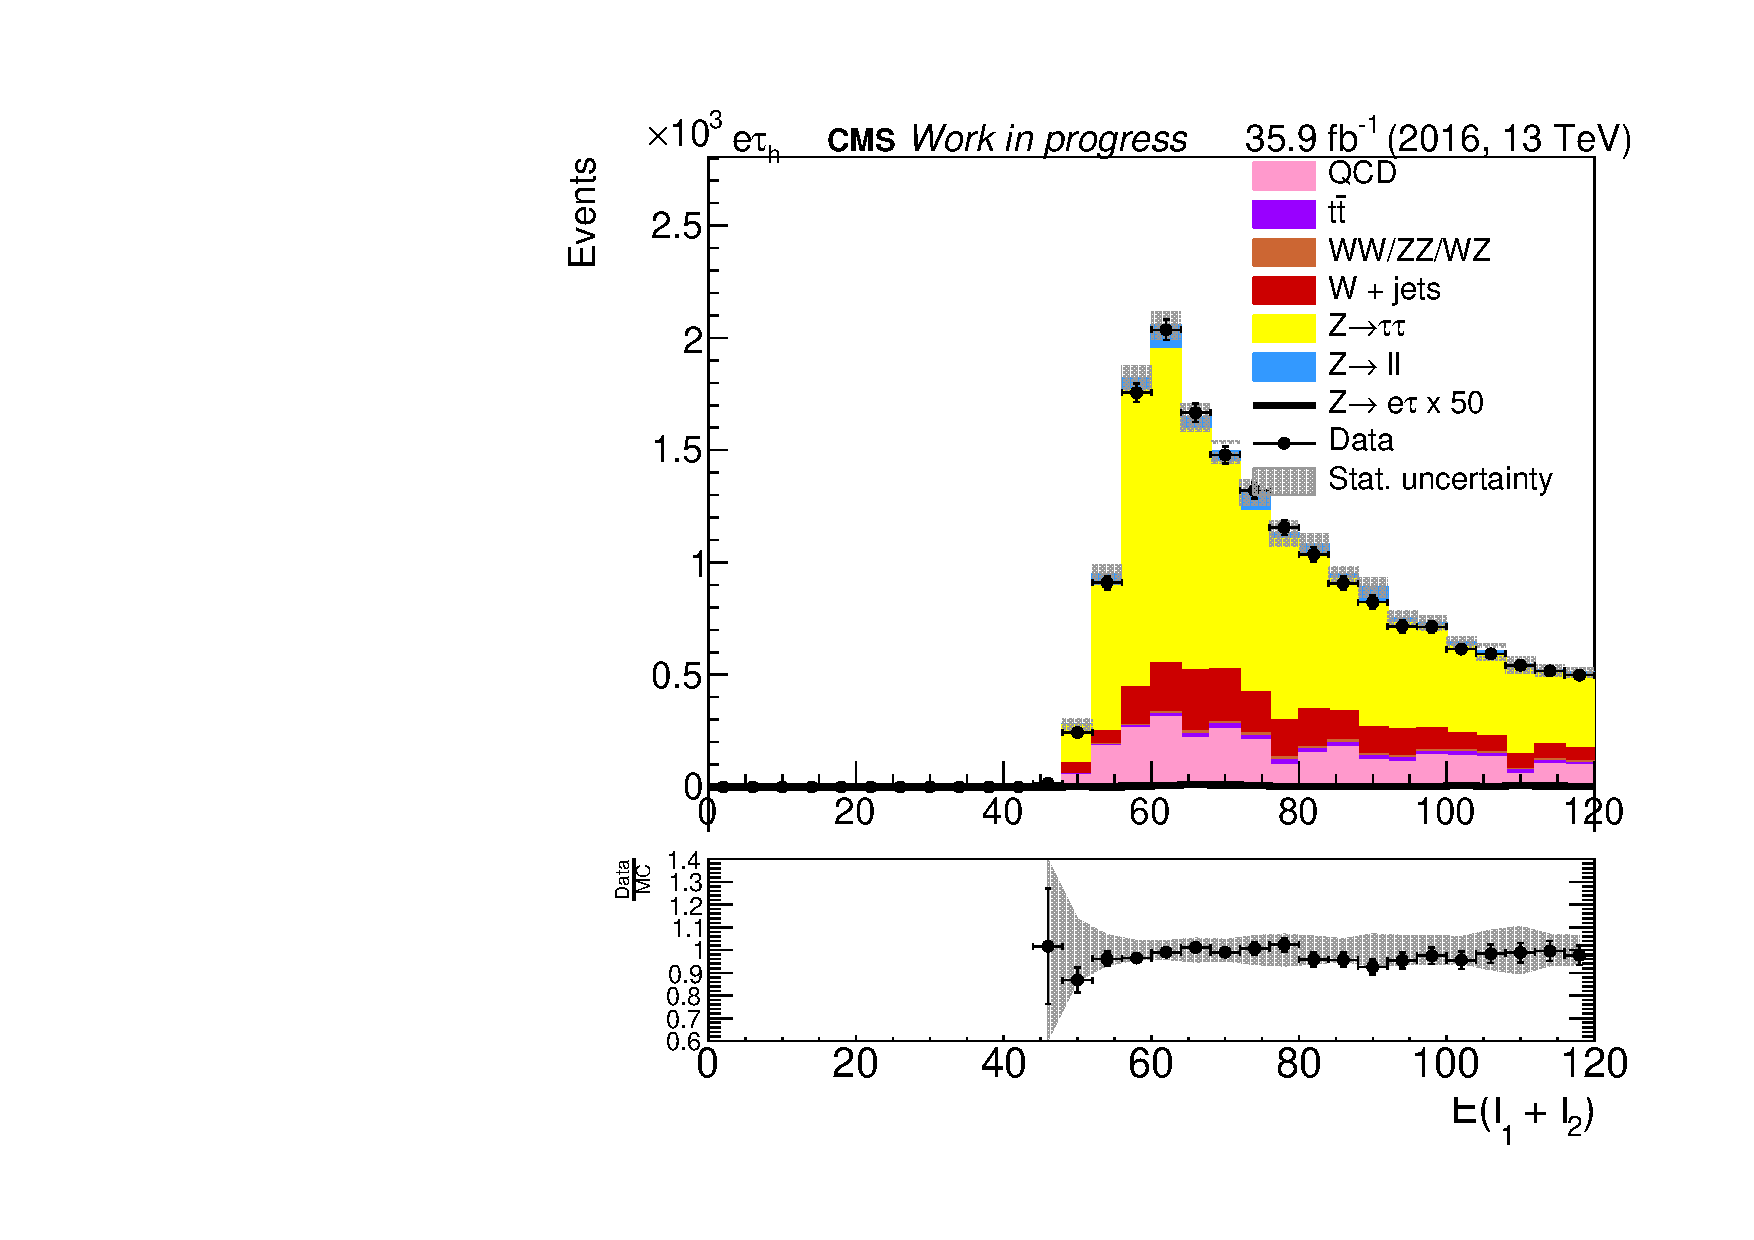
\includegraphics[width=0.45\textwidth]{plots/et/EnergySum_CR.pdf}
	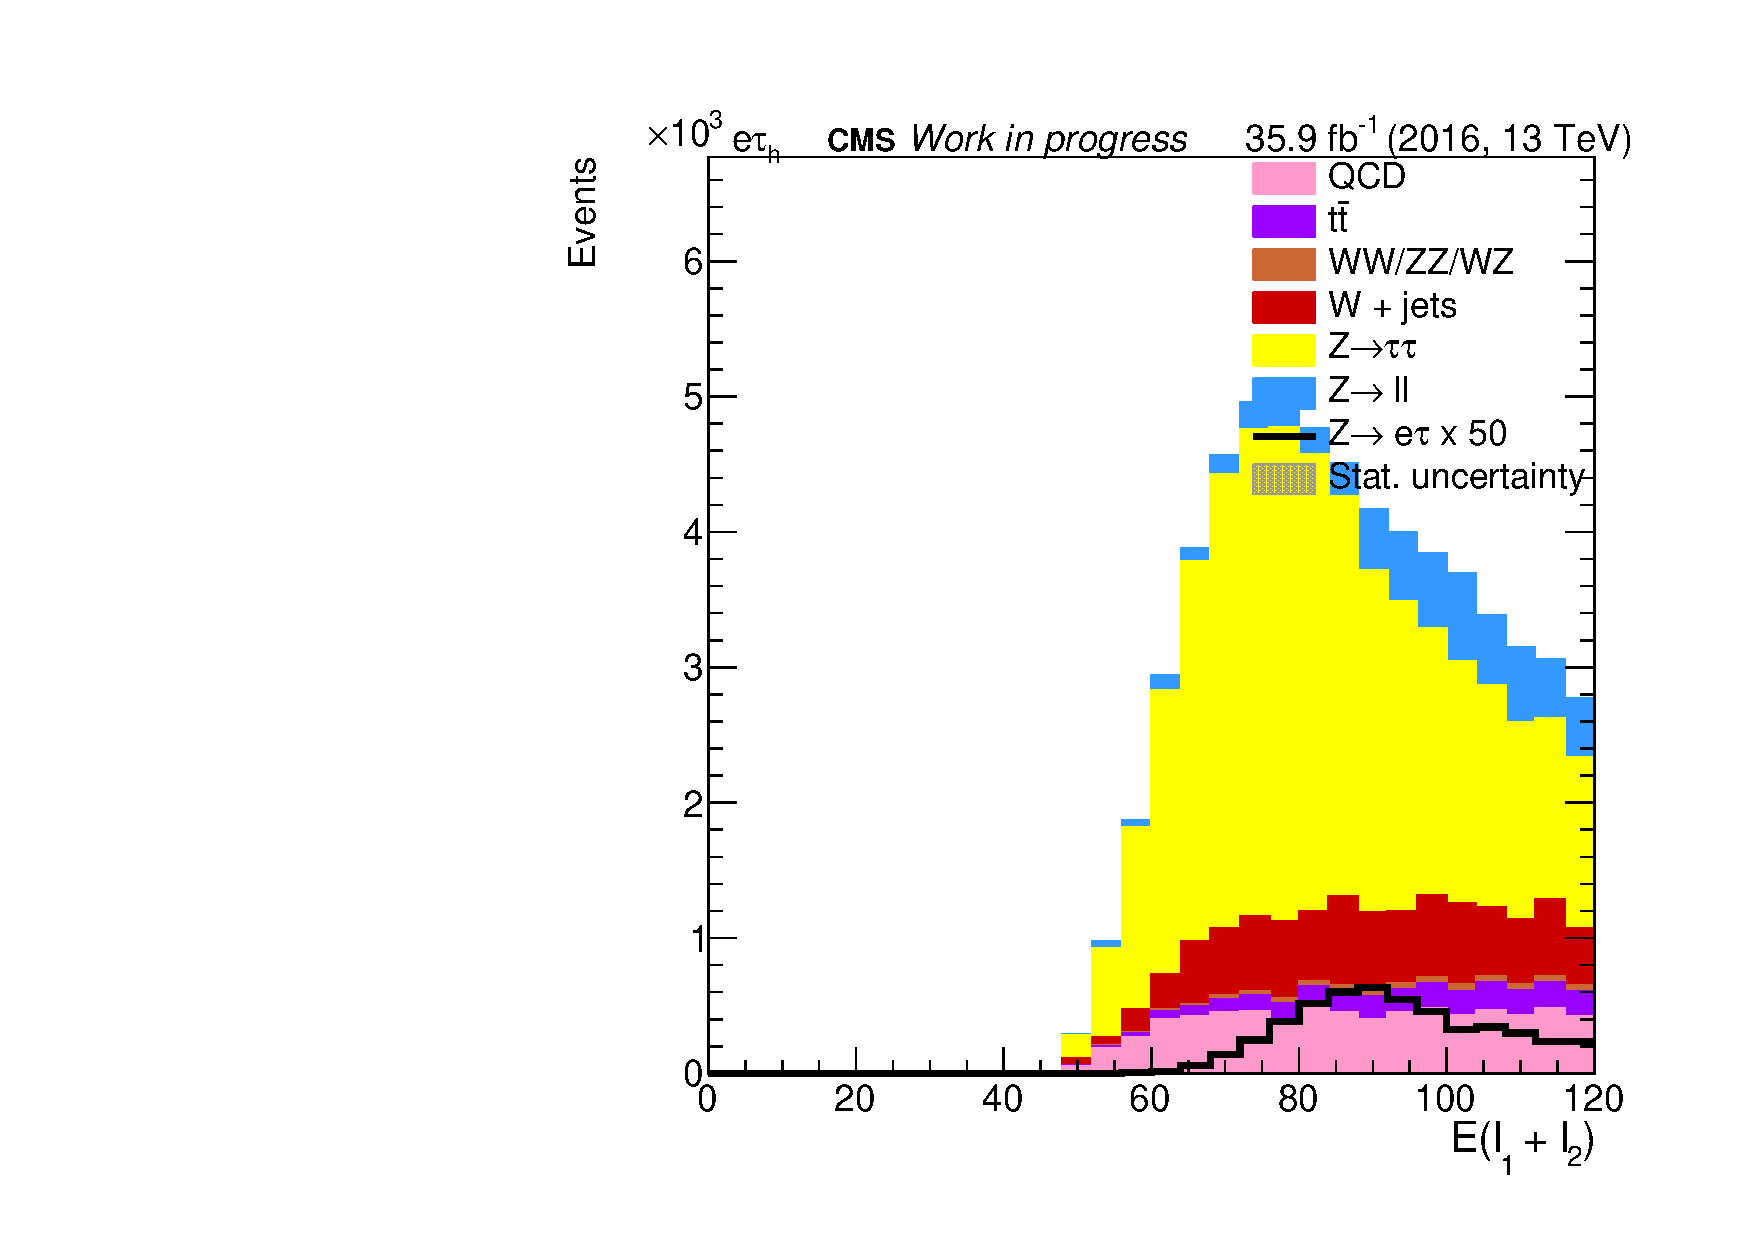
\includegraphics[width=0.45\textwidth]{plots/et/EnergySum_withsignal.pdf}

	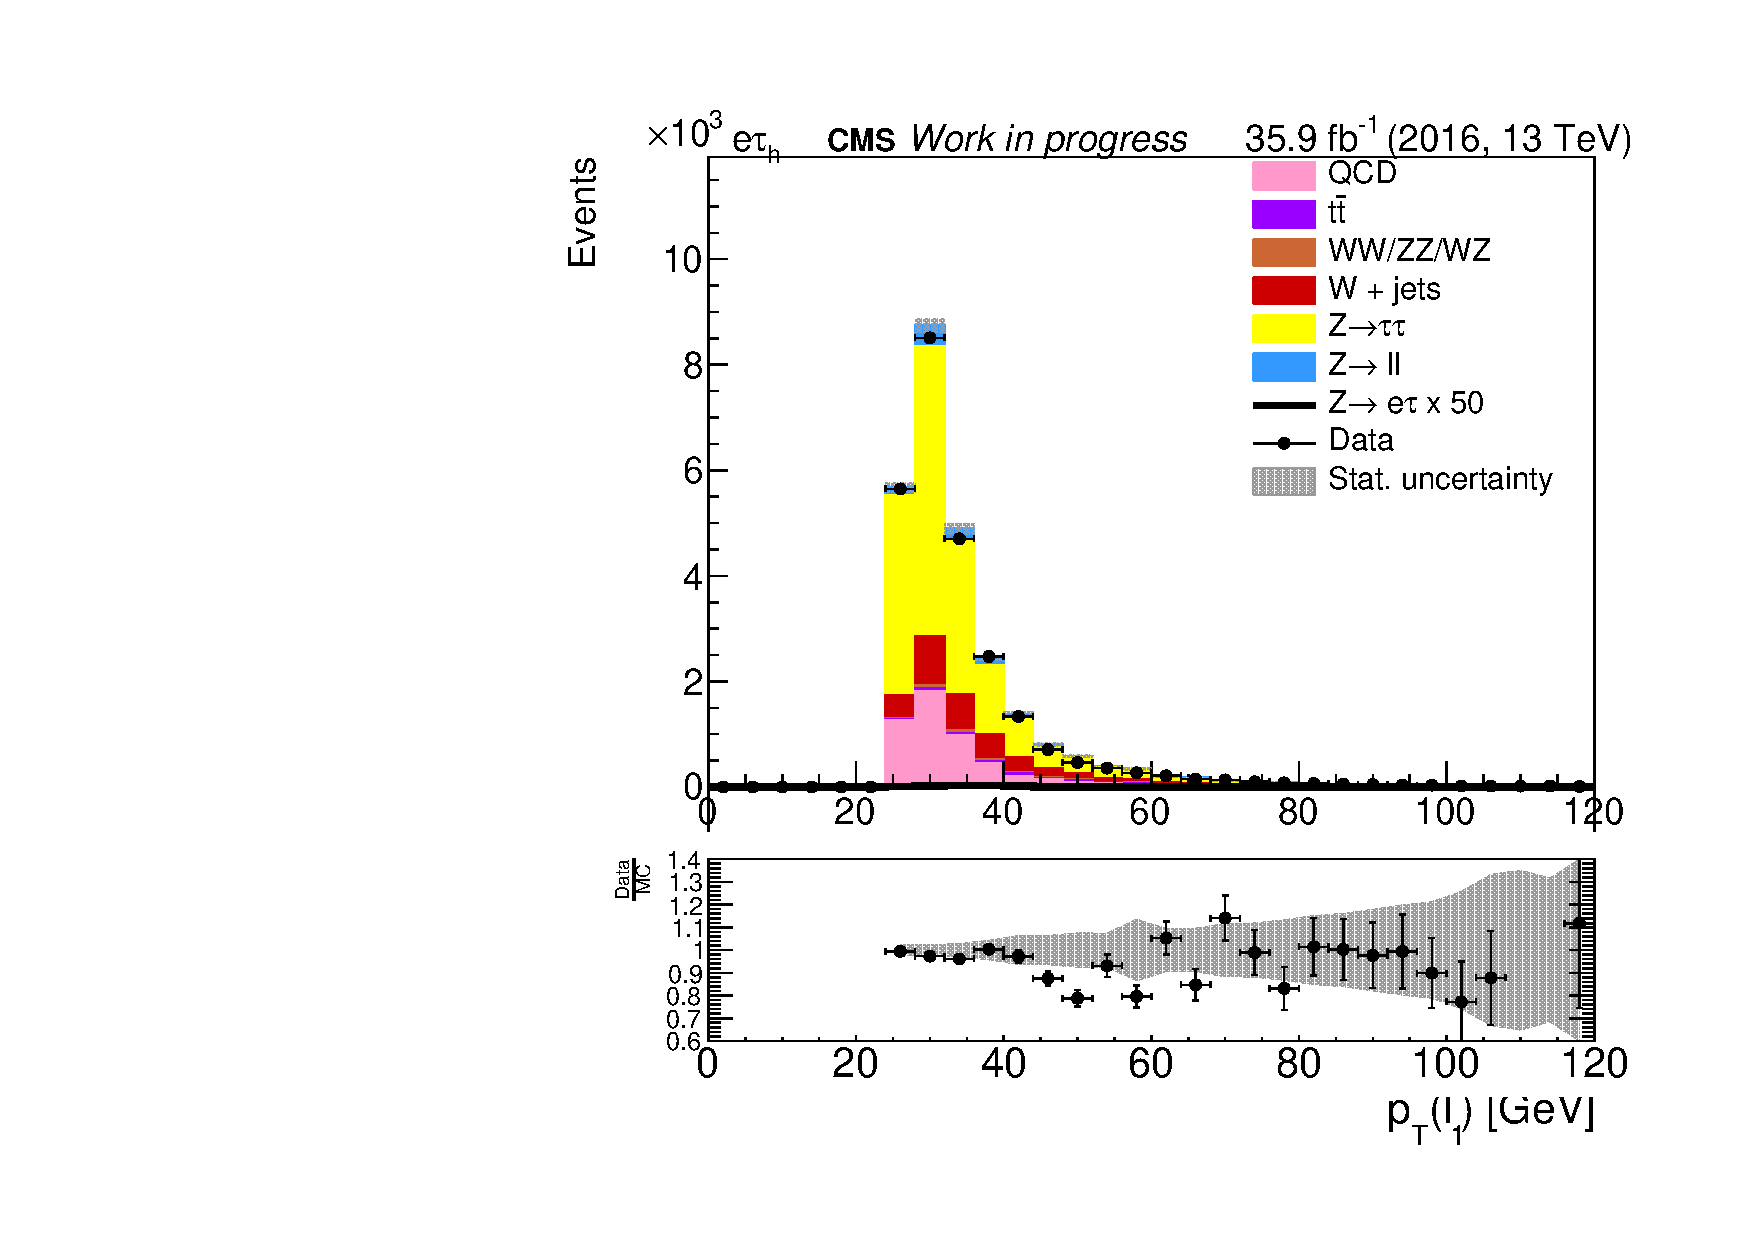
\includegraphics[width=0.45\textwidth]{plots/et/TransverseMomentum1_CR.pdf}
	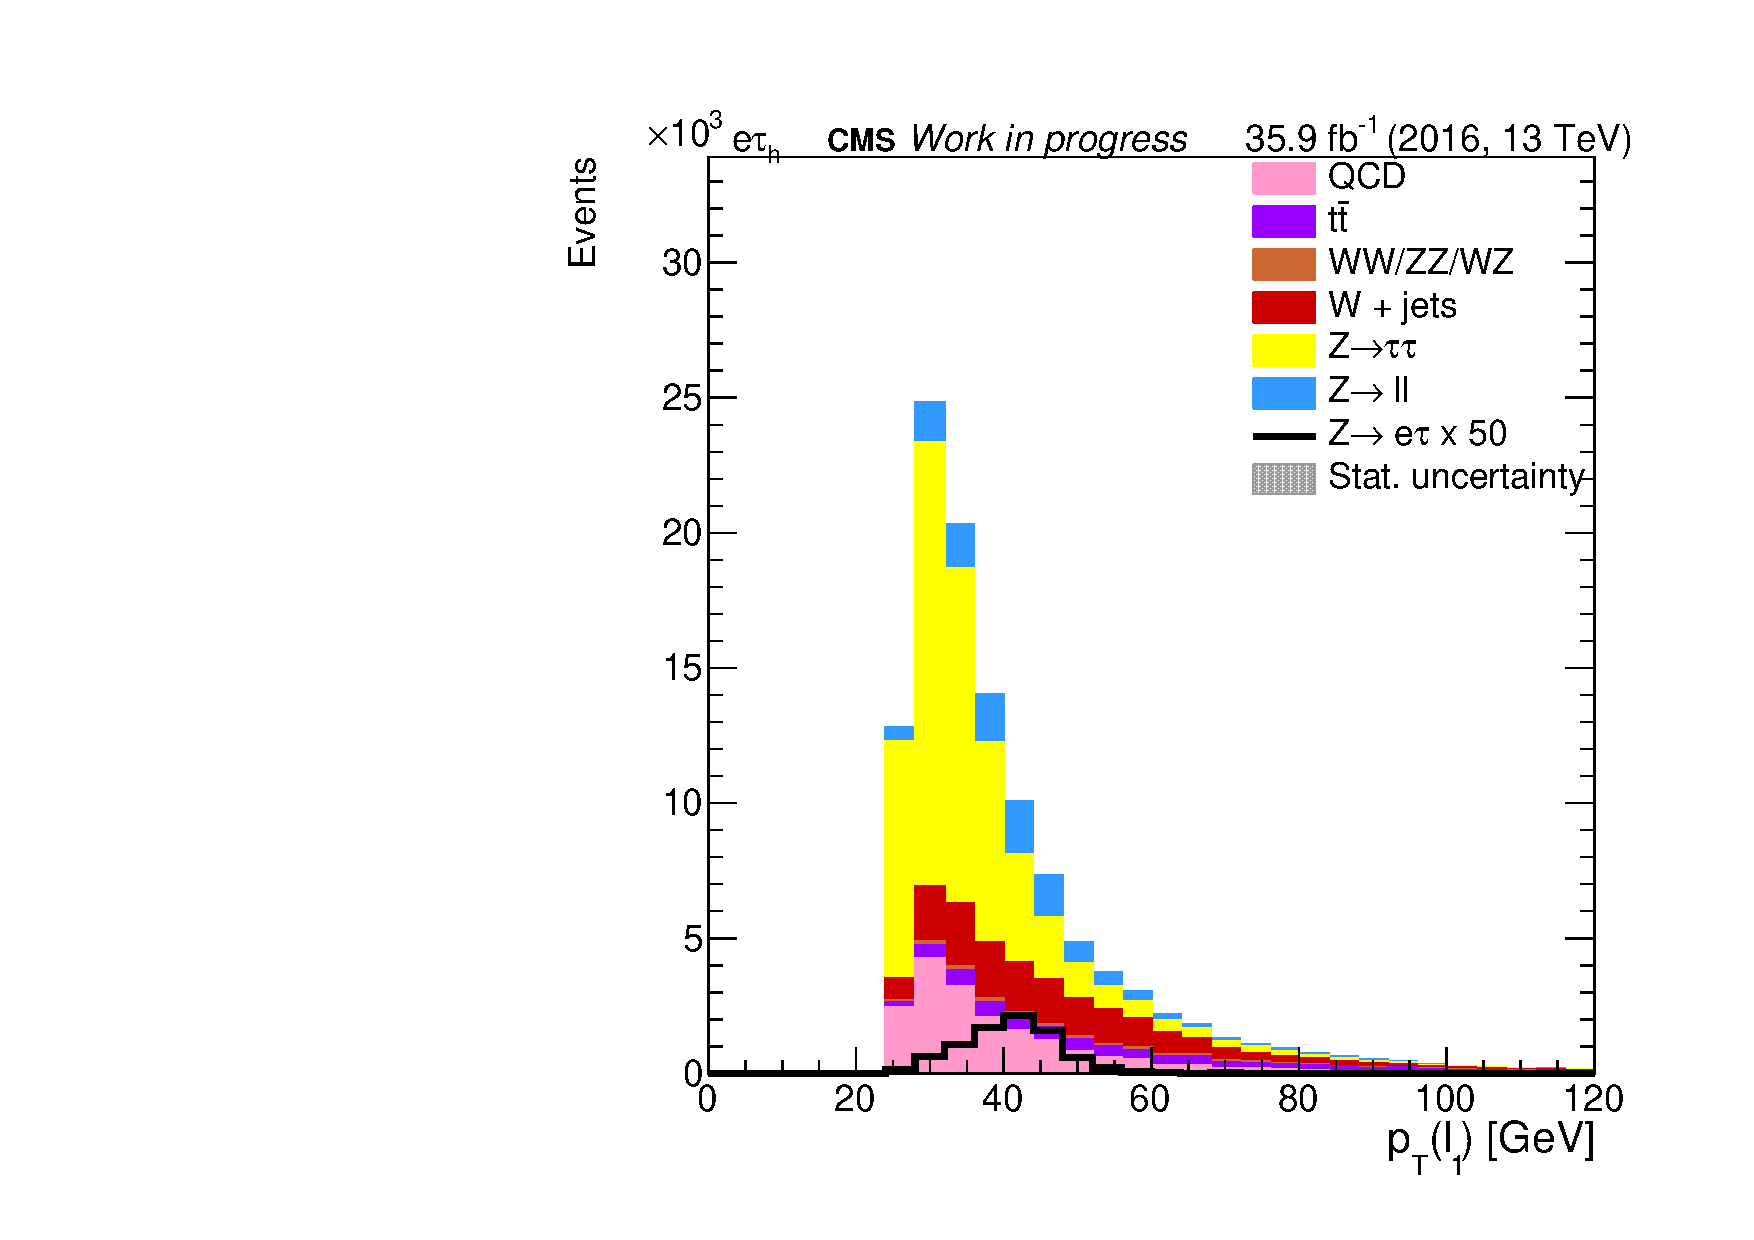
\includegraphics[width=0.45\textwidth]{plots/et/TransverseMomentum1_withsignal.pdf}

	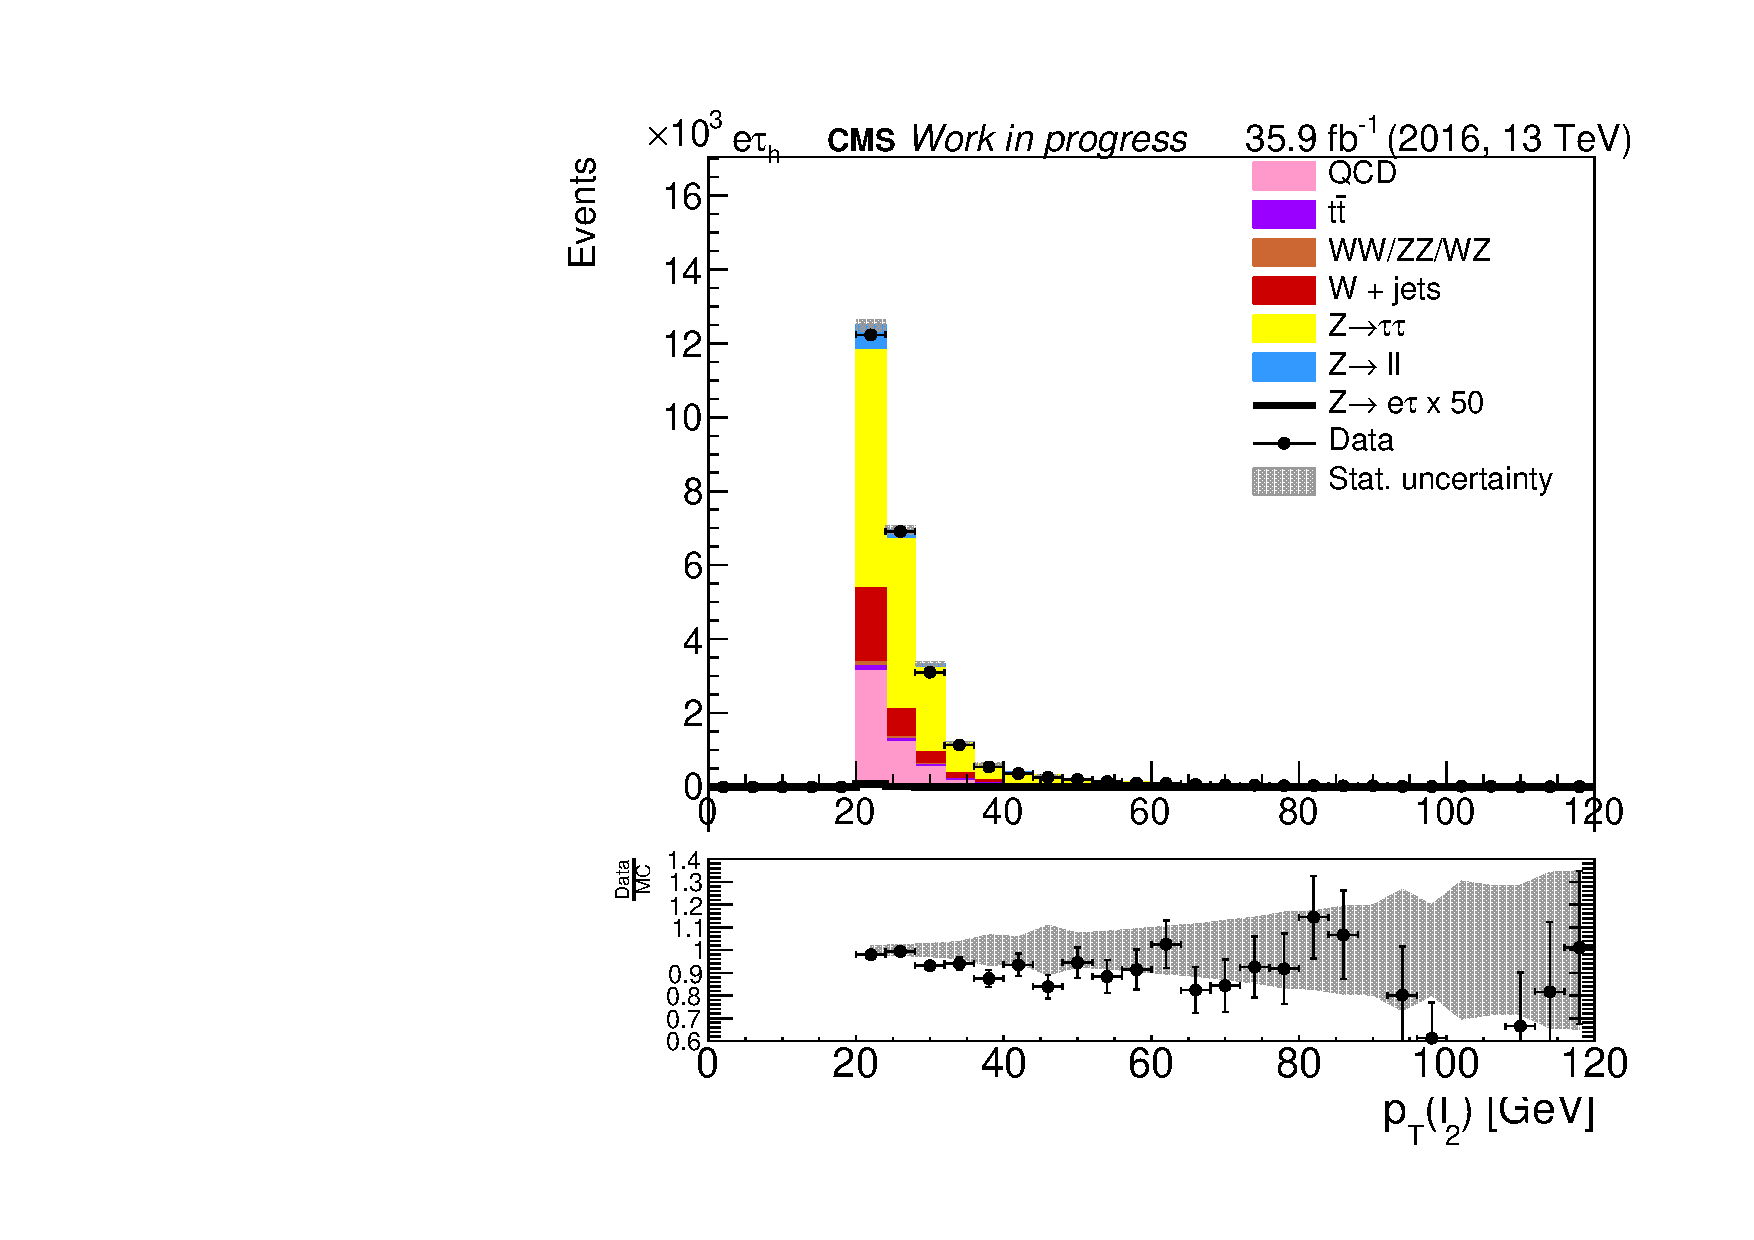
\includegraphics[width=0.45\textwidth]{plots/et/TransverseMomentum2_CR.pdf}
	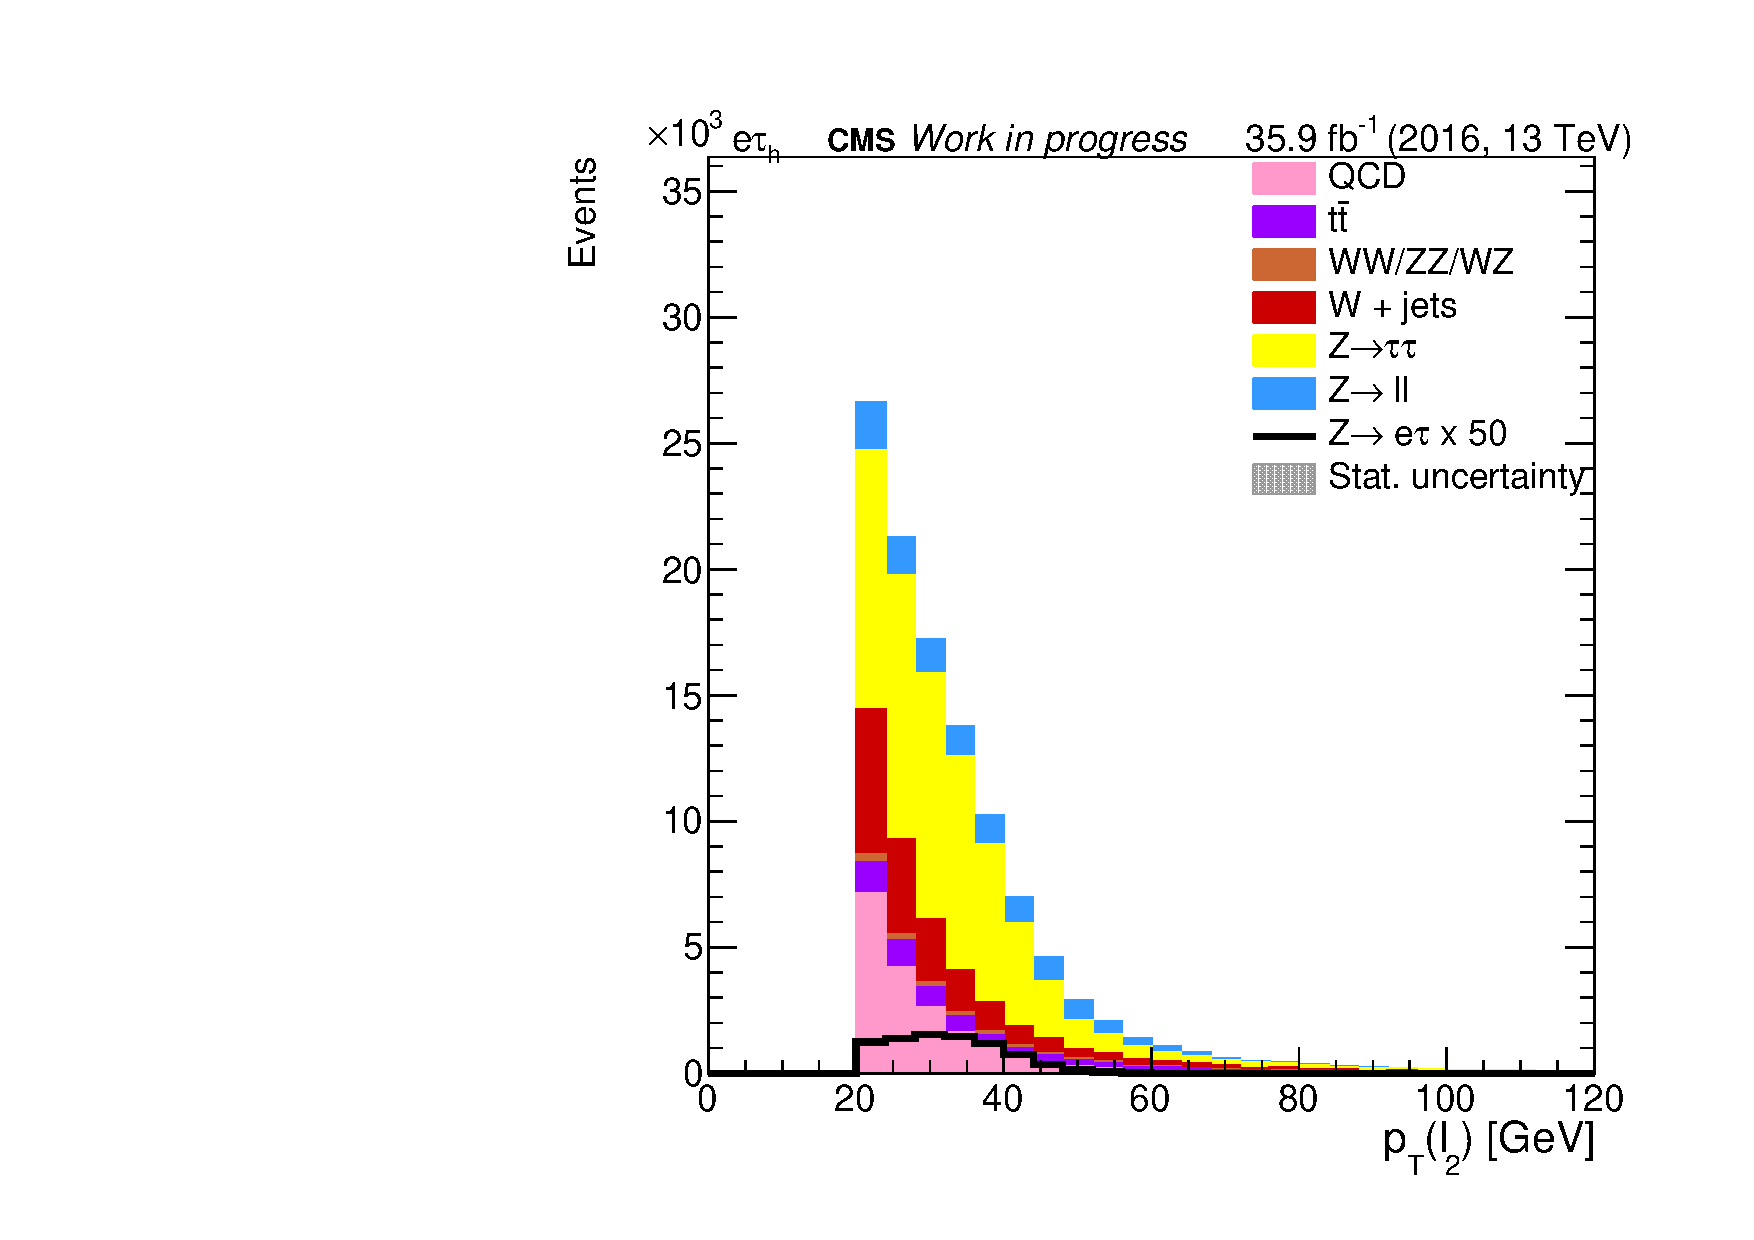
\includegraphics[width=0.45\textwidth]{plots/et/TransverseMomentum2_withsignal.pdf}
\end{figure}


\begin{figure}[htp]
	\includegraphics[width=0.45\textwidth]{plots/et/ImpactParameter1_CR.pdf}
	\includegraphics[width=0.45\textwidth]{plots/et/ImpactParameter1_withsignal.pdf}

	\includegraphics[width=0.45\textwidth]{plots/et/ImpactParameter2_CR.pdf}
	\includegraphics[width=0.45\textwidth]{plots/et/ImpactParameter2_withsignal.pdf}

	\includegraphics[width=0.45\textwidth]{plots/et/MissingTranverseEnergy_CR.pdf}
	\includegraphics[width=0.45\textwidth]{plots/et/MissingTranverseEnergy_withsignal.pdf}
\end{figure}

\newpage

\section*{Plot for the $\mu\tau$ final state}

\begin{figure}[htp]
	\includegraphics[width=0.45\textwidth]{plots/mt/DeltaPhiL1L2_CR.pdf}
	\includegraphics[width=0.45\textwidth]{plots/mt/DeltaPhiL1L2_withsignal.pdf}

	\includegraphics[width=0.45\textwidth]{plots/mt/DeltaPhiL1Z_CR.pdf}
	\includegraphics[width=0.45\textwidth]{plots/mt/DeltaPhiL1Z_withsignal.pdf}

\end{figure}


\begin{figure}[htp]
	\includegraphics[width=0.45\textwidth]{plots/mt/DeltaPhiL2Z_CR.pdf}
	\includegraphics[width=0.45\textwidth]{plots/mt/DeltaPhiL2Z_withsignal.pdf}

	\includegraphics[width=0.45\textwidth]{plots/mt/DeltaPhiMetL1_CR.pdf}
	\includegraphics[width=0.45\textwidth]{plots/mt/DeltaPhiMetL1_withsignal.pdf}

	\includegraphics[width=0.45\textwidth]{plots/mt/DeltaPhiMetL2_CR.pdf}
	\includegraphics[width=0.45\textwidth]{plots/mt/DeltaPhiMetL2_withsignal.pdf}
\end{figure}


\begin{figure}[htp]
	\includegraphics[width=0.45\textwidth]{plots/mt/DiEta_CR.pdf}
	\includegraphics[width=0.45\textwidth]{plots/mt/DiEta_withsignal.pdf}

	\includegraphics[width=0.45\textwidth]{plots/mt/DiLepPt_CR.pdf}
	\includegraphics[width=0.45\textwidth]{plots/mt/DiLepPt_withsignal.pdf}

	\includegraphics[width=0.45\textwidth]{plots/mt/DiTransverseMass_CR.pdf}
	\includegraphics[width=0.45\textwidth]{plots/mt/DiTransverseMass_withsignal.pdf}
\end{figure}


\begin{figure}[htp]
	\includegraphics[width=0.45\textwidth]{plots/mt/EnergySum_CR.pdf}
	\includegraphics[width=0.45\textwidth]{plots/mt/EnergySum_withsignal.pdf}

	\includegraphics[width=0.45\textwidth]{plots/mt/TransverseMomentum1_CR.pdf}
	\includegraphics[width=0.45\textwidth]{plots/mt/TransverseMomentum1_withsignal.pdf}

	\includegraphics[width=0.45\textwidth]{plots/mt/TransverseMomentum2_CR.pdf}
	\includegraphics[width=0.45\textwidth]{plots/mt/TransverseMomentum2_withsignal.pdf}
\end{figure}


\begin{figure}[htp]
	\includegraphics[width=0.45\textwidth]{plots/mt/ImpactParameter1_CR.pdf}
	\includegraphics[width=0.45\textwidth]{plots/mt/ImpactParameter1_withsignal.pdf}

	\includegraphics[width=0.45\textwidth]{plots/mt/ImpactParameter2_CR.pdf}
	\includegraphics[width=0.45\textwidth]{plots/mt/ImpactParameter2_withsignal.pdf}

	\includegraphics[width=0.45\textwidth]{plots/mt/MissingTranverseEnergy_CR.pdf}
	\includegraphics[width=0.45\textwidth]{plots/mt/MissingTranverseEnergy_withsignal.pdf}
\end{figure}
